\documentclass[USenglish]{ifimaster}

\usepackage[export]{adjustbox}
\usepackage[utf8]{inputenc}
\usepackage{ifimasterforside}
\usepackage{graphicx}
\usepackage{float}

\usepackage[acronym, toc]{glossaries}
\usepackage[toc,page]{appendix}

\usepackage[backend=biber,sorting=none]{biblatex}
\usepackage{listings}

\usepackage{tabularx}
\usepackage{cleveref}

% For listings
\usepackage{bera}
\usepackage{listings}
\usepackage{xcolor}
\colorlet{punct}{red!60!black}
\definecolor{background}{HTML}{EEEEEE}
\definecolor{delim}{RGB}{20,105,176}
\colorlet{numb}{magenta!60!black}
\lstdefinelanguage{json}{
    basicstyle=\normalfont\ttfamily,
    numbers=left,
    numberstyle=\scriptsize,
    stepnumber=1,
    numbersep=8pt,
    showstringspaces=false,
    breaklines=true,
    frame=lines,
    backgroundcolor=\color{background},
    literate=
     *{0}{{{\color{numb}0}}}{1}
      {1}{{{\color{numb}1}}}{1}
      {2}{{{\color{numb}2}}}{1}
      {3}{{{\color{numb}3}}}{1}
      {4}{{{\color{numb}4}}}{1}
      {5}{{{\color{numb}5}}}{1}
      {6}{{{\color{numb}6}}}{1}
      {7}{{{\color{numb}7}}}{1}
      {8}{{{\color{numb}8}}}{1}
      {9}{{{\color{numb}9}}}{1}
      {:}{{{\color{punct}{:}}}}{1}
      {,}{{{\color{punct}{,}}}}{1}
      {\{}{{{\color{delim}{\{}}}}{1}
      {\}}{{{\color{delim}{\}}}}}{1}
      {[}{{{\color{delim}{[}}}}{1}
      {]}{{{\color{delim}{]}}}}{1},
}

\definecolor{pblue}{rgb}{0.13,0.13,1}
\definecolor{pgreen}{rgb}{0,0.5,0}
\definecolor{pred}{rgb}{0.9,0,0}
\definecolor{pgrey}{rgb}{0.46,0.45,0.48}
\lstset{language=Java,
  showspaces=false,
  showtabs=false,
  breaklines=true,
  showstringspaces=false,
  breakatwhitespace=true,
  commentstyle=\color{pgreen},
  keywordstyle=\color{pblue},
  stringstyle=\color{pred},
  basicstyle=\ttfamily,
  moredelim=[il][\textcolor{pgrey}]{$$},
  moredelim=[is][\textcolor{pgrey}]{\%\%}{\%\%}
}


\makeglossaries

% Acronyms
\newacronym{acm}{ACM}{Agile Computing Middleware}
\newacronym{afro}{AFRO}{Adaption Framework foR Web Services prOvision}
\newacronym{amqp}{AMQP}{Advanced Message Queuing Protocol}
\newacronym{api}{API}{Application Program Interface}
\newacronym{coap}{CoAP}{The Constrained Application Protocol}
\newacronym{cnr}{CNR}{Combat Net Radio}
\newacronym{cots}{COTS}{Commercial off-the-shelf}
\newacronym{dsproxy}{DSProxy}{Delay and disruption tolerant SOAP Proxy}
\newacronym{dil}{DIL}{Disconnected, Intermittent and Limited}
\newacronym{edge}{EDGE}{Enhanced Data rates for GSM Evolution}
\newacronym{efx}{EFX}{Efficient XML}
\newacronym{ffi}{FFI}{Norwegian Defence Research Establishment}
\newacronym{fec}{FEC}{Forward Error Correction}
\newacronym{ftp}{FTP}{File Transfer Protocol}
\newacronym{http}{HTTP}{Hypertext Transfer Protocol}
\newacronym{ietf}{IETF}{Internet Engineering Task Force}
\newacronym{iot}{IoT}{Internet of Things}
\newacronym{ip}{IP}{Internet Protocol}
\newacronym{jvm}{JVM}{Java Virtual Machine}
\newacronym{los}{LOS}{Line of Sight}
\newacronym{lte}{LTE}{Long-Term Evolution}
\newacronym{manet}{MANET}{Mobile ad hoc network}
\newacronym{mockets}{Mockets}{Mobile Sockets}
\newacronym{mtu}{MTU}{Maximum Transfer Unit}
\newacronym{nato}{NATO}{North Atlantic Treaty Organization}
\newacronym{nec}{NEC}{Network Enabled Capability}
\newacronym{netem}{NetEm}{Network Emulator}
\newacronym{nffi}{NFFI}{NATO Friendly Force Information}
\newacronym{nio}{NIO}{Java new/non-blocking I/O}
\newacronym{ntnu}{NTNU}{Norwegian University of Science and Technology}
\newacronym{oasis}{OASIS}{Organization for the Advancement of Structured
Information Standards}
\newacronym{per}{PER}{Packet Error Rate}
\newacronym{qos}{QoS}{Quality of Service}
\newacronym{rest}{REST}{Representational State Transfer}
\newacronym{satcom}{SATCOM}{Satellite Communication}
\newacronym{sctp}{SCTP}{Stream Control Transmission Protocol}
\newacronym{soa}{SOA}{Service Oriented Architecture}
\newacronym{soap}{SOAP}{SOAP}
\newacronym{std}{STD}{Standard Deviation}
\newacronym{tcp}{TCP}{Transmission Control Protocol}
\newacronym{udp}{UDP}{User Datagram Protocol}
\newacronym{uri}{URI}{Uniform Resource Identifier}
\newacronym{w3c}{W3C}{World Wide Web Consortium}
\newacronym{wsdl}{WSDL}{Web Services Description Language}
\newacronym{www}{WWW}{World Wide Web}
\newacronym{xml}{XML}{Extensible Markup Language}

\title{Improving the performance of Web Services in Disconnected, Intermittent
and Limited Environments}
\author{Joakim Johanson Lindquister}
\bibliography{references}

\begin{document}
\ififorside{}

\chapter*{Abstract}

The goal of this thesis is to investigate different optimization techniques that
can be applied in order to improve Web service performance in \gls{dil}
networks. In order for the clients and services to remain interoperable the
optimization techniques will be placed in proxies. The Web services will
communicate as normal, while all network traffic is tunneled through a proxy.
The Web service itself does not need to pay attention to the bad connectivity,
the proxy will choose the appropriate protocol and configuration.

\chapter*{Preface}

This master thesis was written at the Department of Informatics at the Faculty of Mathematics and Natural Sciences, University at the University of Oslo in 2015/2016. It was written in cooperation with \gls{ffi}, which provided the thesis topic and supervison.


\tableofcontents
\listoftables
\listoffigures

\pagebreak

\chapter{Introduction}

Military units operate under conditions where the reliability of the
network connection may be low. They can operate far from existing communication
infrastructure and rely only on wireless communication. Such networks are
often characterized by unreliable connections with low date rate and high
error rates making data communication difficult. In a military scenario it is
necessary for units at all operational levels to seamlessly exchange
information across different types of communication systems. This ranges from
foot soldiers with radio equipment on a remote battlefield, to the commanding
officer in a far away headquarter full of computers. To \gls{nato}, this
concept is referred to as \gls{nec}. In a feasibility study, \gls{nato}
identified the \gls{soa} paradigm and the Web Service technology as key
enablers for information exchange in \gls{nato}\cite{nnec-study}.

Web Service technology is well tested and in widespread use in civil
applications where the network is stable and the data rate is abundant.
However, certain military networks suffer from high error rates and very low
date rate, which can leave Web Services built for civilian use unusable. This
thesis investigates how these challenges can be overcome by applying  different
optimization techniques. We apply different techniques, the most central one
investigating how using alternative transport protocols than HTTP/TCP may
increase speed and reliability.


\section{Background and Motivation}

\gls{nato} is a military alliance consisting of 28 member countries
\cite{nato-homepage-member-countries} and which primary goal is to protect the
freedom and security of its members through political and military means. In
joint military operations the relatively large number of member countries can be
a challenge when setting up machine-to-machine information exchange. Differences
in communication systems and equipment attribute to making the integration of
such systems more difficult. In order to address this issue, NATO has chosen the
\gls{soa} concept, which when built using open standards facilitates
interoperability\cite{nnec-study}.

\subsection{\glsentrylong{soa}}
\gls{soa} is an architectural pattern where application components
provide services to other components over a network. \gls{soa} is built on
concepts such as object-orientation and distributed computing and aims to get
a loose coupling between clients and services. In their reference model for
\gls{soa}, the \gls{oasis} define \gls{soa} as \cite{oasis-soa-reference-model}:

\paragraph{}

\textit{Service Oriented Architecture is a paradigm for organizing and utilizing
distributed capabilities that may be under the control of different ownership
domains. It provides a uniform means to offer, discover, interact with and use
capabilities to produce desired effects consistent with measurable preconditions
and expectations.} % SOA Trekant figur her

\paragraph{}

In \gls{soa}, business processes are divided into smaller chunks of business
logic, referred to as \textit{services}. A service can be business related, e.g
a patient register service, or a infrastructure service used by other services
and not by a user application. \gls{oasis} define a service as
\cite{oasis-soa-reference-model}:

\paragraph{}
\textit{
A service is a mechanism to enable access to one or more capabilities, where the
access is  provided using a prescribed interface and is exercised consistent
with constraints and policies as  specified by the service description
}

\begin{figure}[h]
\includegraphics[scale=0.6]{images/SOA.png}
\caption{The three roles in SOA(from \cite{ist-090})}
\end{figure}

Services are provided by \textit{service providers} and are consumed by
\textit{service consumers}. The service provider is responsible for creating a
service description, making the service available to others and implementing the
service according to the service description. Services are made available to
service consumers through a form of \textit{service discovery}. This can be a
static configuration, or more dynamic with a central \textit{service registry},
where service providers publish service descriptions. Service consumers find the
services they need by contacting the service registry. The communication between
services occur through the exchange of standardized messages.

Following the \gls{soa} principles dictates a very loose coupling between
services and the consumers of those. This allows software systems to be more
flexible, as new components can be integrated with minimal impact on the
existing system. Another aspect of loose coupling is with regard to time, which
enable services and its consumers to not be available at the same instance of
time. This enables asynchronous communication. Loose coupling with regards to
location allows the location of a service to be changed without needing to
reprogram, reconfigure, or restart the service consumers. This is possible
through the usage of service discovery, which is dynamic retrieval of the new
location of the service.

Furthermore \gls{soa} enables service implementation neutrality. The
implementation of service is completely separated from the service
description. This allows re-implementation and alteration of a service without
affecting the service consumers. Thus this can attribute to keep development
costs low and avoiding proprietary solutions and vendor lock-in. Another
benefit with \gls{soa} is re-usability by dividing common business processes
into services, which may help cost reduction and avoids duplication. \gls{soa}
is only a pattern and the concepts can be realized by a range of technologies.
The most common used approach is the Web service family of standards, using
the SOAP messaging protocol.

To achieve interoperability between systems from different nations and vendors,
NATO has chosen the Web Service technology in order to realize the \gls{soa}
principles\cite{soa-baseline}. This allows member nations to implement their own
technology as long as they adhere to the standards. The Web service technology
is discussed in detail in \cref{web-services}. Another approach to realize
\gls{soa} is \gls{rest}, an architecture style which uses HTTP over TCP.
\gls{rest} has gained a lot of traction in the civil industry and is discussed
in section \cref{rest}.


\subsection{Military Networks}

Military networks are complex and consist of many different heterogeneous
network technologies. We can group them into layers which have different
characteristics as can been seen in \cref{figure:military-networks}. At the
highest level, there is fixed infrastructure and relatively static users,
meaning that they seldom move around or disconnect. At the lower levels, there
are fewer units, but they are much more dynamic. The lower level is called
tactical networks, which is discussed in the next paragraph.

\begin{figure}[h]
\includegraphics[scale=0.4, left]{images/network_complexity.png}
\caption{Complexity of military networks(from \cite{pervasive-web})}
\label{figure:military-networks}
\end{figure}

\subsubsection{Tactical Networks}
Tactical networks are characterized by that the units are deployed to operate in
a battlefield, which means there is no existing communication infrastructure.
They use tactical communication equipment, which includes technologies like VHF,
UHF, HF, tactical broadband and satellites\cite{ist-090}.
% Mangler referanse på bruk av satelitter.

Examples of such units are mobile units like vehicles, foot soldiers and field
headquarters. The tactical network connects deployed headquarters with mobile
units. These types of networks are unpredictable and may have very low date
rate, possibly high delay, high error rates and frequent disconnections. They
are often called disadvantaged grids or \gls{dil} environments, which is the
term used in this thesis. \gls{dil} is discussed in \cref{dil}.

NATO studies\cite{nato-disadvantaged-grids} have identified such networks to
have the following characteristics:
\\\\
\textit{
Disadvantaged grids are characterized by low bandwidth, variable throughput,
unreliable connectivity, and energy constraints imposed by the wireless
communications grid that link the nodes
}.
\paragraph{}
The characteristics of these networks and what challenges they impose are
discussed in further detail in \cref{dil}.


%%%%%%%%%% DIL %%%%%%%%%%%%%%%
\subsection{\glsentrylong{dil} Networks}
\label{dil}

To improve the performance of Web services in limited military networks, we
must understand what limitations we're dealing with. The \gls{dil} concept refers
to three characteristics of a limited network. As we discussed in the
introduction, military tactical networks may suffer from these constraints.

\begin{description}
\item[Disconnected]
Military units that participate in a tactical network are highly mobile
and may disconnect from a network either voluntarily or not. This causes
topology changes. Unplanned loss of connectivity can be due to various reasons,
such as loss of signal or equipment malfunction.  The disconnected term refers
to that nodes in the network may be disconnected for a long time, possibly for
multiple days.

\item[Intermittent]

Nodes in a \gls{dil} environment may lose connection temporarily before
reconnecting. The duration range from seconds to minutes.

\item[Limited] The Data rate, how many bits that are sent per second, is limited
in \gls{dil} networks. Various aspects that affects the date rate are discussed
in the next section.

\end{description}

\subsubsection{Other constraints}

As well as being restricted  by the communication link itself, military units
may have other limitations as well. Consider that military foot patrols have
limited battery capacity as they have to carry it with them in their
backpacks. The transmission range of the communication equipment for mobile
units may also be limited. Another factor that comes into play for military
units is that in some cases they are required to enter radio silence in order
to avoid being detected by the enemy. During such circumstances the soldiers
may only receive data, but not send any.


\subsubsection{Network metrics}

Network metrics are used to describe various aspects of data transfer from a
point to another.

\begin{description}

\item[Link throughput] The link throughput is influenced by how large distance
there is between the units communicating.

\item[Link reliability] How much of the arriving data that is correct. This is
called \textit{bit error rate} or \textit{packet error rate}. With high error
rates, more data to be transmitted again due to the data arriving being
incorrect. This contributes to longer transmission time. In a military setting,
an enemy may deliberate sabotage the network with jamming, causing higher error
rates.

\item[Link latency] The communication technology in use influences how fast data
transmission can be done. Long delay may cause that the application sending data
timing out.

\end{description}


\section{Example scenario}

Jeg tenkte her å introdusere et scenario som illustererer problemer og utfordringer
med DIL nettverk.


\subsection{Employing proxies}

The Web service technology enables interoperability between systems, but also
increase the information overhead, requiring higher data rate demands. Employing
Web Services developed for use in civilian networks directly into a \gls{dil}
environment may not perform satisfactorily. To increase the performance we can
apply optimization techniques. There are many approaches and optimization
techniques which can be applied at different levels of the protocol stack. In
the coming sections the different optimization techniques are presented and a
overview is presented in \Cref{table:optimalization-overview}. Another issue
that needs to be addressed is, when we have identified optimization techniques,
where do we place them? In the application itself or in a proxy?

One approach is to modify the Web service application itself. However, this
would mean that every application that is used in a tactical network would
require modification. This would require a lot of resources and severely limit
the flexibility of using Web services. Another solution is, by using proxies, we
can place the optimization there without altering the Web Services themselves.
The only thing required to do is to setup the application to send and receive
data through the proxy. The proxy will take care of the optimization for
tactical networks. This seems like a more reasonable approach and is explored in
this thesis.


\section{Problem Statement}
Most of the Web service solutions used today are aimed for civilian use and do
not necessarily perform well in military environments. In contrast to civilian
networks where the date rate is abundant, mobile tactical networks may suffer
from high error rates and low date rate. Adapting Web service solutions meant
for civil networks directly for military purposes may not be possible.
Therefore, Web services needs to be adapted in order to handle network
challenges. However, it can be very expensive to alter existing Web service
technology and incorporate proprietary solutions. A NATO research task group has
previously identified the foundation on open standards to avoid tighter coupling
between service providers and consumers\cite{ist-090}. It is much better to use
\gls{cots} software. By placing the optimization in proxies, the
Web Services can remain unchanged.

The goal of this thesis is to investigate different optimization techniques that
can be applied in order to improve Web service performance in \gls{dil}
networks. In order for the clients and services to remain interoperable the
optimization techniques will be placed in proxies. The Web services will
communicate as normal, while all network traffic is tunneled through a proxy.
The Web service itself does not need to pay attention to the bad connectivity,
the proxy will choose the appropriate protocol and configuration.

\section{Premises}
\begin{itemize}

\item The Web services should not be required to be customized, all
optimization should be placed in proxies.

\item Platform independent?

\item Applications that are to be used in military networks need to be approved
by security authorities. If the application is too complex, e.g.  a very large
code base or use a lot of external frameworks, the approvement process will be
very lengthy. It is therefore a premises that the proxy is relatively simple.

\end{itemize}

\section{Scope and Limitations}

The goal of this thesis is to investigate optimization techniques for Web
services in \gls{dil} environments. Security is therefore not addressed in this
thesis. However, some security features such as IPSec will be enabled or
disabled as part of the evaluation of the proxy.

The proxy implemented as a part of this thesis, will be a HTTP-proxy. As we
will discuss later in \cref{web-services}, most Web services use HTTP.

\section{Research Methodology}
Denning.


\section{Contribution}

The outcome of this thesis is a recommendation regarding which optimizations
techniques, which can be used in DIL to enhance the performance of Web services.
As well as a prototype implementation of a DIL proxy.

\section{Outline}
Hvordan er resten av oppgaven strukturert.

\chapter{Technical Background}

\label{chapter:background}



Before diving into the design and implementation of the proxy developed in this
thesis, in this chapter we present the technical background of the central
concepts and protocols. We first give an introduction to computer networks in
general and how they are organized. Then we look into two very common
communication patterns. Next, we discuss common Web services used for exchanging
data in military systems. Then we look into a number of protocols that we can
replace HTTP/TCP with in order to increase the performance of Web services.
Finally, we introduce the concept of performance testing and network metrics.

\section{Computer Networks}

A computer network allows computers to exchange data. The most common is the
Internet, which allows computers all over the world to communicate. In this
section we give an introduction to protocol suite of the Internet, discuss some
common messaging pattern, before we define discuss performance testing in
general.

\subsection{Network Layers}

To reduce design complexity, networks are organized into layers, each one built
upon the one below it. In the Internet Protocol Suite\cite{rfc-1122}, networks
are divided into 4 layers. As stated in the scope of this thesis, we only look
into optimization techniques for the application and transport layer.

%%%%%%%%%%%% Internet Protocol Suite %%%%%%%%%%%%%%%%%%%
\begin{table}[h]
\begin{tabularx}{\textwidth}{| X |}
\hline
  \textbf{Application Layer} \\ \hline
  \textbf{Transport Layer} \\ \hline
  \textbf{Internet Layer} \\ \hline
  \textbf{Link layer} \\ \hline
\end{tabularx}
\caption{The layers of the Internet Protocol Suite}
\label{figure-network-layers}
\end{table}

\subsubsection{Link Layer}

The lowest layer is the link layer, where link refers to the physical
network component used to interconnect nodes in a network. Link layer protocols
operate between adjacent network nodes. An example of a link layer protocol is
Ethernet.

\subsubsection{Internet Layer}

 Where the link layer is only concerned of moving data over a wire to an
 adjacent node, the Internet layer is concerned of how to deliver data all the
 way from a source to a destination, possible passing through multiple nodes on
 its way. It does not guarantee delivery of data, since data can be lost on the
 way to the destination. Guaranteed delivery is usually handled on the higher
 levels of the Internet Protocol Suite.

 The core protocol of the Internet layer is the \gls{ip} and its routing function
 enables sending data over interconnected networks.

\subsubsection{Transport Layer}

In the Internet protocol suite model, the transport layer provides end-to-end
communication services for applications. It builds on top of the network layer,
and takes responsibility for sending data all the way from a process on a source
machine to a process on the destination machine. The by far most used transport
protocol is the \gls{tcp}, which provides reliable transport of data to
applications. With reliable transport we mean that if data in transmission is
lost or received in the wrong order, this is all handled by the transport
protocol. This provides an important abstraction for applications so that they
don't need to deal with the characteristics of the physical network itself.

\subsubsection{Application Layer}

The top layer of the Internet Protcol Suite is the application layer. Its role
is to serve communication services to applications. When we talk about
application layer protocols, we usually talk about protocols that applications
use to communicate with other applications. Application layer protocols use the
communication services the transport layer provides. Examples of application
layer protocols are \gls{http} and the \gls{ftp}, which both rely on \gls{tcp}
as the underlying transport protocol.

\subsection{Messaging Patterns}

A message pattern describes how applications communicate data with each other.
This data is referred to as \textit{messages}. There exist multiple messaging
patterns and in this chapter we look into protocols using two very common
approaches:

\subsubsection{Request-Response}

Request-response is a message pattern where a requester sends a request to a
system. The system then process the request and responds with a response
message.

\subsubsection{Publish-Subscribe}

Publish-subscribe is a message pattern where subscribers express their interest
in a type of messages, often called topics or classes. A message publisher then
creates messages of a certain class and publish them without needing to know who
are actually subscribing to these types of messages. Many publish-subscribe
system employ a \textit{message broker} as seen in
\cref{figure-message-brokers}. The message broker handles published messages
from publishers and receives subscriptions from subscribers. The broker can
perform various tasks, such as message filtering and prioritize queuing.

\begin{figure}[h]
\centering
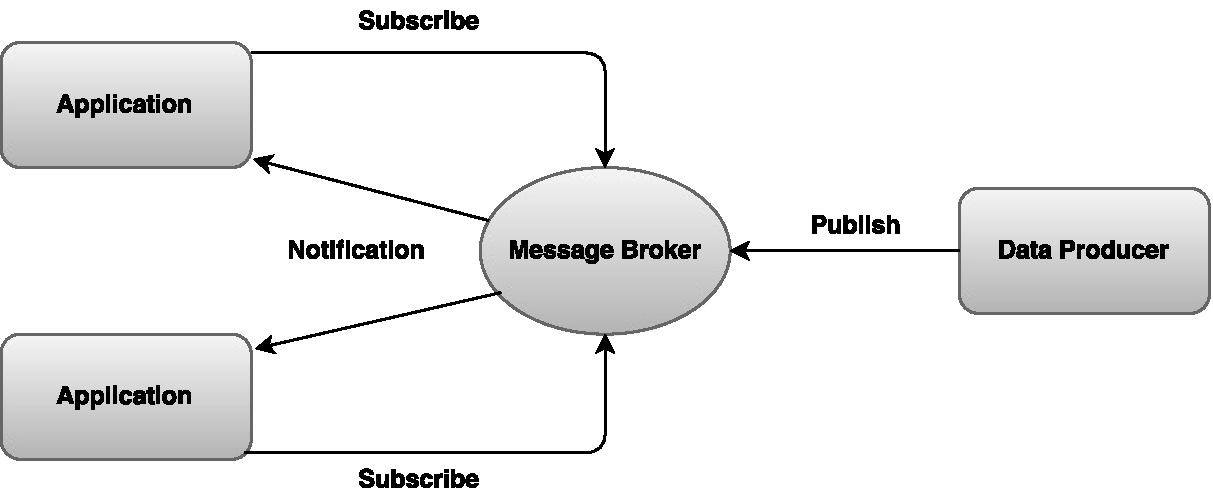
\includegraphics[scale=0.6]{images/pubsub.pdf}
\caption{Message Brokers}
\label{figure-message-brokers}
\end{figure}


\subsection{Performance Testing}

To determine which optimization techniques that have a positive effect on the
performance of Web services in DIL environments, we do performance testing.

\subsection{Network Metrics}

Network metrics are used to describe various aspects of data transfer from a
point to another.

\begin{description}

\item[Data throughput] The data throughput is influenced by how large distance
there is between the nodes communicating.

\item[Reliability] How much of the arriving data that is correct. This is
called \textit{bit error rate} or \textit{packet error rate}. With high error
rates, more data to be transmitted again due to the data arriving being
incorrect. This contributes to longer transmission time. In a military setting,
an enemy may deliberate sabotage the network with jamming, causing higher error
rates.

\item[Latency] The communication technology in use influences how fast data
transmission can be done. Long delay may cause that the application sending data
times out.

\end{description}


\section{Web Services}
\label{web-services}

Web services are client and server applications that communicate over a network.
They can be used to realize the \gls{soa} priniciples, and are in widespread use
in both civilian and military systems. It is worth noting that the term \textit{Web
services} is a broad term and can be used to describe different types of
services available over a network. The most common usage of the term refers to
the \gls{w3c} definition of SOAP-based Web services, but could also refer to
more simple HTTP-based \gls{rest} services.

In this thesis we investigate optimization techniques that should support both
\gls{w3c} Web services and \gls{rest}ful web services.

\subsection{W3C Web Services}

\gls{w3c} has defined Web services as \cite{wrc-web-service}:

\paragraph{}
\textit{
    A Web service is a software system designed to support interoperable
    machine-to-machine interaction over a network. It has an interface described in
    a machine-processable format (specifically WSDL). Other systems interact with
    the Web service in a manner prescribed by its description using SOAP-messages,
    typically conveyed using HTTP with an XML serialization in conjunction with
    other Web-related standards.
}

\paragraph{}

This definition points out a set of standards that enable machine-to-machine
interactions. Web service interfaces is described in documents called WSDL, and
communication is based on sending XML-based SOAP messages. There exists many
definitions of Web services where the core principles are the same, but the
finer details may vary. \Cref{figure-w3c-web-services} illustrates these
fundamental principles. Web service technology is a realization of the \gls{soa}
principles, which provides loose coupling and eases integration between systems.

\begin{figure}[h]
\centering
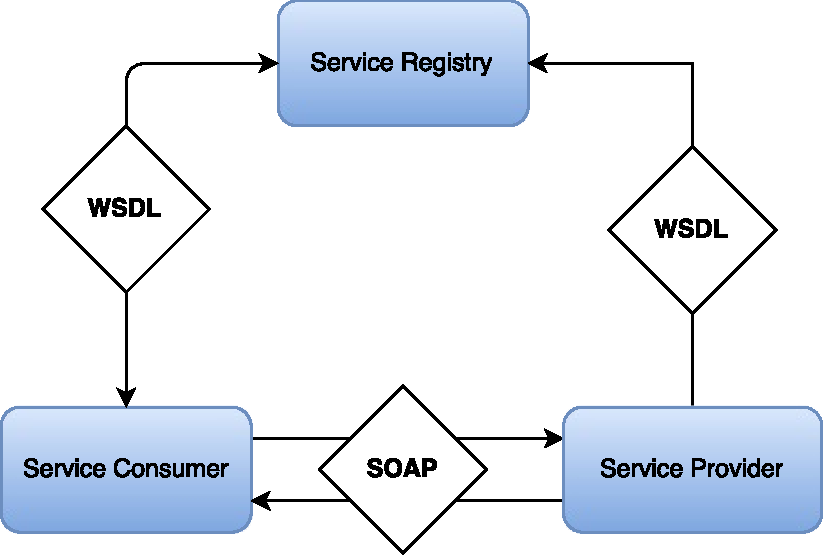
\includegraphics[scale=0.6]{images/web_services.pdf}
\caption{W3C Web services}
\label{figure-w3c-web-services}
\end{figure}

These standards that together make W3C Web services are presented in the
following sections.

\subsubsection{\glsentrylong{xml}}

The \gls{xml}\cite{W3C-XML} is considered as the base standard for Web services.
An XML document consist of data surrounded by tags and is designed to be both
machine and user readable. Tags describe the data they enclose. The tags can be
standardized, which allows exchange and understanding of data in a standardized,
machine-readable way.


\subsubsection{\glsentrylong{wsdl}}

\gls{wsdl} is an XML-based interface definition language that describes
functionality offered by a Web service \cite{w3c-wsdl}. The interface describes
available functions, data types for message requests and responses, binding
information about the transport protocol, as well as address information for
locating the service. This enables a formal, machine-readable description of Web
service which clients can invoke.

\subsubsection{SOAP}

SOAP is an application level, XML-based protocol specification for information
exchange\cite{w3c-soap} in the implementation of Web services. Data
communication in SOAP is done by nodes sending each other whats called SOAP
messages. A SOAP message can be considered as an "envelope" consisting of an
optional message header and a required message body. The header can contain
information not directly related to the message such as routing information for
the message and security information. The body contains the data being sent,
known as the payload.

SOAP is transport protocol agnostic, which means it can be carried over various
underlying protocols. The far most used transport protocol is HTTP over TCP, but
other protocols such as UDP and SMTP can be used as well.

\subsection{\glsentrylong{rest}}
\label{rest}

In the previous sections we looked into the standards and specifications that
compose W3C Web services. However, there also exist other types of Web services
which do not follow the these standards. In 2000, the computer scientist Roy
Fielding introduced \gls{rest} where he presented a model of how he thought the
Web \textit{should} work. This idealized model of interactions within a Web
application is what we refer to as the REST architectural style
\cite{rest-fielding}. REST attempts to minimize latency and network
communication while maximizing the independence and scalability of component
implementations. This is done by placing constraints on connector semantics
rather than on component semantics like W3C Web services.  REST is based on a
client-server model where a client requests data from a server when needed.

Web services that adhere to the REST style are called RESTful Web services. They
are closely associated with HTTP and use HTTP verbs(e.g GET, POST, DELETE) to
operate on information located on a server. RESTful Web services typically
expose some sort of information, called resources in REST. \Cref{table-rest}
illustrates how a component exposes a set of operations of an example car
resource. Resources are identified by a resource identifier. While W3C Web
services are service oriented, we can look at REST as being more resource
oriented.

 %%%%%%%%%%%% REST eksempel %%%%%%%%%%%%%%%%%%%
 \begin{table}[h]
 \begin{tabularx}{\textwidth}{| X | X | X |}
 \hline
   \textbf{Resource identifier} & \textbf{HTTP Method}  & \textbf{Meaning}\\ \hline
   /vehicles/cars/1234 & GET & Return a car with ID 1234 from the system. \\ \hline
   /vehicles/cars/ & POST & Create a new car which will be added to the list of cars. \\ \hline
   /vehicles/cars/1234 & DELETE & Delete a car with ID 1234 from the system. \\ \hline
 \end{tabularx}
 \caption{Example of REST operations}
 \label{table-rest}
 \end{table}

 \gls{rest} is easy to understand and has gained a lot of traction in the civil
 industry in the latest years. Although NATO has chosen W3C Web services as the
 technology to do information exchange, REST is identified as a technology of
 interest to certain groups in NATO \cite{johnsen-recommendations}. One potential
 downside to NATO with REST however, is that RESTful Web services lack
 standardization, which may cause interoperability issues.

Closely associated with REST and the most used transport protocol for W3C Web
services are \gls{http}, which we present in detail in the next section.


\section{\glsentrylong{http}}

As we have seen in the previous sections, both RESTful and W3C Web services
utilize the \gls{http} as their way to communicate with other services. The
usage of \gls{http} is very widespread and it is the foundation of data
communication for the \glsentrylong{www} since the early 90's. It's protocol
specification is coordinated by \gls{ietf} and the \gls{w3c}, and is defined
as \cite{rfc-2616}:

\paragraph{}
\textit{
    The Hypertext Transfer Protocol (HTTP) is an application-level
    protocol for distributed, collaborative, hypermedia information
    systems. It is a generic, stateless, protocol which can be used for
    many tasks beyond its use for hypertext, such as name servers and
    distributed object management systems, through extension of its
    request methods, error codes and headers
}

\paragraph{}

\gls{http} started out as a simple protocol for raw data transfer across the
Internet and has since been updated in HTTP/1.0, HTTP/1.1 and most recently a
major update with HTTP/2.0. It is a request-response protocol which means that all
data exchanges are initiated with a client invoking a HTTP-request and then
waits until a server responds with a HTTP response. A HTTP-request consist of
the request method, \gls{uri}, protocol version, client information, and a optional
body. The server responds with a message containing a status line, protocol
version, a code indicating the success or error of the request, and a optional
body. Both HTTP requests and responses use a generic message format and can
contain zero or more HTTP headers. Headers are used to provide information about
the request/response or about the message body, e.g information about the encoding
and caching information.

HTTP, being an application level protocol, relies on a transport protocol to
actually transfer data to an another machine. HTTP communication most often, but
not necessarily, occurs over TCP/IP connections. The only requirement in the HTTP
specification is that a reliable transport protocol is used.

\subsection{HTTP Methods}

 Associated with all HTTP requests is a request method, which indicates the
 desired action to be performed on a resource located on a Web server. The set
 of HTTP methods defined in HTTP/1.1 is listed in \cref{table-http-methods}.

 %%%%%%%%%%%% HTTP methods %%%%%%%%%%%%%%%%%%%
 \begin{table}[h]
 \begin{tabularx}{\textwidth}{| X | X |}
 \hline
   \textbf{HTTP Method} & \textbf{Purpose} \\ \hline
   OPTIONS & Asks the server which HTTP methods and header field it supports. \\ \hline
   GET & Retrieve information identified by the resource indentifier(Request-URI). \\ \hline
   HEAD & Identical to GET, except that the HTTP-body is not returned from the server. \\ \hline
   POST & Asks the server to accept the message payload from the client as a new resource.\\ \hline
   PUT & Similar to POST but allows the client to ask the server to update a resource identified by the request-uri \\ \hline
   DELETE & Requests that the resource identified by the request-uri is deleted \\ \hline
   TRACE & Echoes the HTTP request. Used for debugging \\ \hline
   CONNECT & For use with a proxy that can dynamically switch to being a tunnel\\ \hline
 \end{tabularx}
 \caption{HTTP methods}
 \label{table-http-methods}
 \end{table}

\section{\glsentrylong{tcp}}
\label{tcp}

\gls{tcp} is called the workhorse of the Internet because it is so critical for
how the Internet works. It is the primary transport protocol of the Internet
Protocol Suite\cite{rfc-1122} and provides reliable, in-sequence delivery of
two-way traffic(full-duplex) data.  \gls{tcp} was defined in RFC
793\cite{rfc-793} back in September 1981 and has since been improved in various
RFC's. The main motivation behind \gls{tcp} was to provide reliable end-to-end
byte streams over unreliable networks.  HTTP most often uses TCP as its
transport protocol. In this section we present the characteristics of TCP and
some of the issues we may encounter working with it.

 \subsection{The Protocol}

 TCP is a connection-oriented protocol, which means that a connection between a
 sender and the receiver must be established before any data can be transfered.
 A connection is specified by a pair of sockets identifying its two sides.
 Associated with each connection TCP initialize and maintains some status
 information for each connection. This includes window size, socket information
 and sequence numbers.

Computers supporting TCP have a piece of software which manages TCP streams and
interfaces to the IP layer. Most often this software is a part of the
kernel \cite{computer-networks}. It accepts data streams from local processes,
and breaks them up into pieces, before sending them to the IP layer. The pieces
are called TCP segments, which consist of a fixed 20 byte header, followed by
zero or more data byte. The TCP software decides how big the segments should be,
but for performance reasons they should not exceed the \gls{mtu} of the link(the
physical network). Each segment should be so small that it can be sent in a
single, unfragmented package over the entire network. This usually limits the
size of each segment to the \gls{mtu} of the Ethernet, which is 1500 bytes.

When the TCP software receives data from applications, it is not necessarily
sent immediately as it may be buffered before its sent. At the receiver, data is
delivered to the TCP software, which reconstructs the original byte streams and
deliver them to the target application.


\subsection{TCP Reliability}

When transferring data over the Internet, the data may pass through various
networks, routers and physical networks. Some of the routers may not work
correctly, a bit may be flipped when transferring data wirelessly, or some other
factor may come in to play. For those reasons, we have to accept that some of
the data will be damaged, lost, duplicated or delivered out of order.

TCP recovers from such faults by assigning sequence number to each packet being
sent. It then requires a positive acknowledgement from the receiver that the
data was actually received. If the acknowledgement is not received within a
timeout interval, the data is transmitted again. For the receiver the sequence
numbers are used to ensure that data is received in the correct order, as well
as eliminating duplicates. Furthermore, to detect damaged data, TCP applies
checksums to each segment transmitted. At the receiver the checksum is then
checked and damaged segments are discarded.

\subsection{Flow Control}

If a fast receiver sends data faster than a slow receiver is able to process,
the receiver will be swamped with data and may experience serious performance
reduction. Flow control is a mechanism to manage the rate of the data
transmission to avoid overflowing a receiver. TCP provides this by using a
window of acceptable sequence numbers that the receiver is willing to accept.
With every acknowledgement sent back to the sender, the window is specified.
This allows the receiver to control which segments, and how fast, the sender
can send.

\subsection{Congestion Control}

Congestion control is about controlling the data traffic entry into a network in
order to avoid network congestion. On its way from the sender to the receiver,
an IP packet may pass through different subnets with different capabilities.
Network congestion may occur if a node in a network receives more data then it
is able to pass forward. The consequence of this is that an increase in network
traffic to this node, would only lead to a small increase, or even a decrease,
of the network throughput \cite{Al-Bahadili2012}.

To avoid congestion TCP uses a number of mechanisms. These aim to control the
rate of data packets entering into the networks to avoid congestion, but still
get as high throughput as possible. One of these mechanisms is
\textit{slow-start}, which general idea is to start transmitting with a low
packet rate, then gradually increasing the packet rate. When TCP notice that a
packet is eventually lost, it considers it as a sign of network congestion and
reduces its packet rate.

\subsection{Issues Using TCP in DIL}
\label{section:tcp-problems}

DIL networks are characterized by their high delay, low data rate and relatively
high error rate. Since TCP's congestion control interprets this as evidence of
congestion, it will back off and use a lower data rate. This causes TCP to send
with a lower rate than the network actually can provide. Moreover, it could also
ultimately lead to the TCP connection terminating due to those
effects \cite{nato-disadvantaged-grids}.


\section{Protocols of Interest}

Since \gls{tcp} may be sub-optimal or even break down entirely in DIL networks,
we're in this thesis looking into alternative protocols and other optimization
techniques. In networks with low data rate, protocols with low overhead per IP
packet is beneficial. With frequent disconnects, protocols that are
connection-less may be more suitable than connection-oriented. One important
limitation is that NATO has chosen the "everything over IP", which means that
all optimization must occur on the top of the network layer. Because of this we
evaluate protocols in the transport and application layer of the Internet
Protocol Suite.

In the following sections we give a short introduction to the protocols
we're investigating in this thesis. The protocols have been selected because of
their prevalence in the civil and military world or their reported performance
in the "Internet of Things". We get started by discussing \gls{udp}, which
alongside \gls{tcp} is one of the core protocols of the Internet protocol suite.


\subsection{\glsentrylong{udp}}

The Internet has two main protocols in the transport layer, namely \gls{udp} and
\gls{tcp}. They have fundamentally different characteristics and use cases,
which we go through in this section. \gls{udp} was formally defined in 1980 in
RFC 768\cite{rfc-udp} and is a simpler protocol than \gls{tcp}. It sends
messages, called datagrams, to nodes over the \gls{ip} network. While \gls{tcp}
provides reliable transmission along with flow control and congestion control,
do UDP only support the sending of IP datagrams. Furthermore it is a
connectionless protocol, which means that the protocol can send messages
\textit{without} establishing a connection first. Since \gls{udp} does not
provide guaranteed delivery or in-order delivery of messages, it should only be
used by applications that do not require this.

To summarize, \gls{udp} is a more lightweight protocol than TCP. It has smaller
headers and less overhead, which makes it a faster protocol. The downside is
that it does not provide any mechanisms for congestion control or reliability.
UDPs lack of end-to-end congestion control may result in drastic unfairness if
an \gls{udp} stream are competing with a \gls{tcp}
stream \cite{floyd-congestion}. While a TCP stream will detect congestion and
back-down its traffic, an UDP stream will greedily send at full-throttle, thus
causing an unfair share of the available network. UDP is therefore often
referred to as not \textit{TCP-Friendly}.

 It is worth noting that UDPs lack of reliability may by handled on a higher
 level in the application stack on top of \gls{udp}. This is done by the next
 protocol we're looking into.

\subsection{\glsentrylong{coap}}

\gls{coap} is a specialized Web transfer protocol designed for use with
constrained nodes and  networks \cite{rfc-7252}. It is intended for
machine-to-machine applications typically found in the Internet of Things.
Furthermore, it is designed with a similar interface as HTTP in order to easily
integrate with Web services. \gls{coap} and HTTP work similar in the way that
they both use a client-server interaction model. \Gls{coap} is based on the REST
style where a server makes resources available under a \gls{uri}. Clients can
then interact with these resources using a subset of the HTTP-verbs: GET, PUT,
POST and DELETE.

CoAP messaging is based on asynchronously exchanging CoAP messages over UDP
between two endpoints. The current specification defines four types of CoAP
messages, where each message uses a 4 byte fixed-length binary header.
\Cref{table:coap-messages} lists the four types of CoAP messages. A CoAP header
may be followed by \textit{options} and a payload. \Gls{coap} provide mechanisms
for optional reliability since \gls{udp} itself does not guarantee reliable
delivery. This is done by sending messages marked as \textit{Confirmable}, and
retransmitting using a default timeout and exponential back-off until an
\textit{Acknowledgement message} is eventually received. Basic congestion
control is done by strictly limiting the number of allowed outstanding requests
between a client and a server. The back-off mechanism also provides basic
congestion control.

\begin{table}[h]
\centering
\begin{tabularx}{\textwidth}{|X|X|}
\hline
\textbf{CoAP message}   & \textbf{Purpose}                                                                                                  \\ \hline
Confirmable Message     & CoAP message that  requires an acknowledgement. Used to provide reliable transport.                               \\ \hline
Non-confirmable Message & Used when no acknowledgement is wanted.                                                                           \\ \hline
Acknowledgement Message & Acknowledges that a specific Confirmable Message has arrived.                                                     \\ \hline
Reset Message           & Indicates that a Confirmable Message or a Non-confirmable Message was received, but not understood by the client. \\ \hline
\end{tabularx}

\caption{CoAP messages}
\label{table:coap-messages}
\end{table}

Typical CoAP messages may be small payloads from Internet of Things devices such
as temperature sensors, light switches etc. The CoAP specification states that a
CoAP message \textit{should} fit within a single IP packet to avoid IP
fragmentation. However, occasionally larger messages are needed. Therefore a
blockwise transfer technique has been proposed as an extension to CoAP in an
Internet Draft \cite{draft-coap-blockwise}. The block option allows for sending
larger messages in a block-wise fashion.

\subsection{\glsentrylong{amqp}}

The \gls{amqp} is an application layer protocol for sending messages.
It supports both the request/response and the publish/subscribe communication
paradigms. \gls{amqp} uses \gls{tcp} as its underlying reliable transport layer
protocol.

An important observation about AMQP is that it has two major versions which are
fundamentally different, version 0.9.1 and 1.0. The latter has been standardized
by \gls{oasis}, and is a  more narrow protocol as it only defines the network
wire-level protocol for the exchange of messages between two endpoints
\cite{oasis-amqp}. The concept wire-level protocol refers to the description of the format
of data sent over a network in form of bytes. Another difference between the
versions is that version 1.0 does not specify the details of broker
implementation. We investigate version 1.0 since it is the newest and has been
standardized.

An AMQP network consist of nodes connected via \textit{links}. Nodes can be
producers, consumers and queues. Producers generate messages, consumers process
messages, while queues store and forward them. These nodes live inside
\textit{containers}, which can be client applications and brokers. Each
container can have multiple nodes. AMQP version 1.0 is does not specify the
internal workings of those nodes, but defines the protocol for transferring
messages between them. The basic data unit in AMQP is called a \textit{frame}
and is used to initiate, control and tear down the transfer of a message between
two nodes. The 9 different frames are listed in \cref{table-amqp-frames}.

Prior to any communication, an AMQP connection must be established making AMQP a
connection-oriented protocol. A connection is divided into independent
unidirectional \textit{channels}. An AMQP \textit{session} correlates two
unidirectional channels to form a bidirectional, sequential conversation between
two containers. To establish a connection the first operation is to establish a
TCP connection between the nodes. Then the protocol header is exchanged,
allowing the nodes to agree on a common protocol version. This is exchanged in
plaintext (not in an AMQP frame). The message itself is sent with the
\textit{transfer} frame. Larger messages can be split into multiple frames.


\begin{table}[h]
\begin{tabularx}{\textwidth}{| X | X |}
\hline
  \textbf{AMQP Frame} & \textbf{Purpose} \\ \hline
  Open & Describes the capabilities and limits of the node. \\ \hline
  Begin & Begin a session on a channel \\ \hline
  Attach & Attach a link to a session \\ \hline
  Flow & Update link state \\ \hline
  Transfer & Transfer a message \\ \hline
  Disposition & Inform remote peer of delivery state changes \\ \hline
  Detach & Detach the link endpoint from the session \\ \hline
  End & End the session\\ \hline
  Close & Signal a connection close\\ \hline
\end{tabularx}
\caption{AMQP Frames}
\label{table-amqp-frames}
\end{table}

\subsection{MQTT}

MQTT is a publish/subscribe messaging transport protocol \cite{oasis-mqtt}.  It
emerged in 1999 and recently became an \gls{oasis} standard in 2014. MQTT is
considered to be light weight and simple to implement, making it suitable for
use in networks where the data rate is limited and/or a low code footprint is
needed. With the emerge of "The Internet of Things", these properties have
caused regained interest in MQTT. The protocol is broker-based and runs on top
of the TCP/IP protocols.

The protocol provides message sending services to applications and offers
different levels of \gls{qos}, specifying the delivery policies for a message.
This is beneficial in networks where messages may be lost while traveling
through a network. The lowest level of \gls{qos} is \textit{at most once}, which
specifies that a message should arrive at the receiver either once or not at
all. Next, the policy \textit{at least once} ensures that the message arrives at
the receiver at least once, but possible multiple times. The last and highest
level of MQTT's \gls{qos}, \textit{exactly once}, guarantees one, and only one,
delivery of the message. The protocol works by sending different MQTT control
packets, listed in \cref{table:mqtt-packets}. Only \textit{exactly once}
\gls{qos} requires the usage of the control packets PUBREC, PUBREL and PUBCOMP.

\begin{table}[h]
\begin{tabularx}{\textwidth}{| X | X |}
\hline
  \textbf{MQTT Control Packet} & \textbf{Purpose} \\ \hline
  CONNECT & Client requests a connection to the Server \\ \hline
  CONNACK & Acknowledge connection request \\ \hline
  PUBLISH & Publish a message \\ \hline
  PUBACK & Publish acknowledgement \\ \hline
  PUBREC &  Publish received \\ \hline
  PUBREL & Response to a PUBREC Packet \\ \hline
  PUBCOMP & Publish complete \\ \hline
  SUBSCRIBE & Subscribe to topics \\ \hline
  SUBACK & Subscribe acknowledgement\\ \hline
  UNSUBSCRIBE & Unsubscribe from topics\\ \hline
  UNSUBACK & Unsubscribe acknowledgement \\ \hline
  PINGREQ & PING request \\ \hline
  PINGRESP & PING response \\ \hline
  DISCONNECT & Disconnect notification \\ \hline
\end{tabularx}
\caption{MQTT Control packets}
\label{table:mqtt-packets}
\end{table}


\subsection{\glsentrylong{sctp}}

The \glsentrylong{sctp} is a transport-layer protocol, which offers
functionality from both \gls{udp} and \gls{tcp}\cite{rfc-sctp}. The motivation
behind the protocol was that many developers found TCP too limiting, but still
required more reliability that UDP could provide. \gls{sctp} tries to solve
these issues. It is message-oriented like UDP, but ensures reliable, in sequence
transport of messages with congestion control like TCP. \gls{sctp} is a
connection-oriented protocol and provide features like multi-homing and
multi-streaming. Multi-homing is the possibility to use more than one network
path between two nodes. This increases reliability since if one path fails,
messages can still be sent over the other link(s). Multi-streaming refers to
\gls{sctp} ability to transmit several independent streams of data at the same
time, for example sending an image at the same time as a HTML Web page.

\begin{figure}[h]
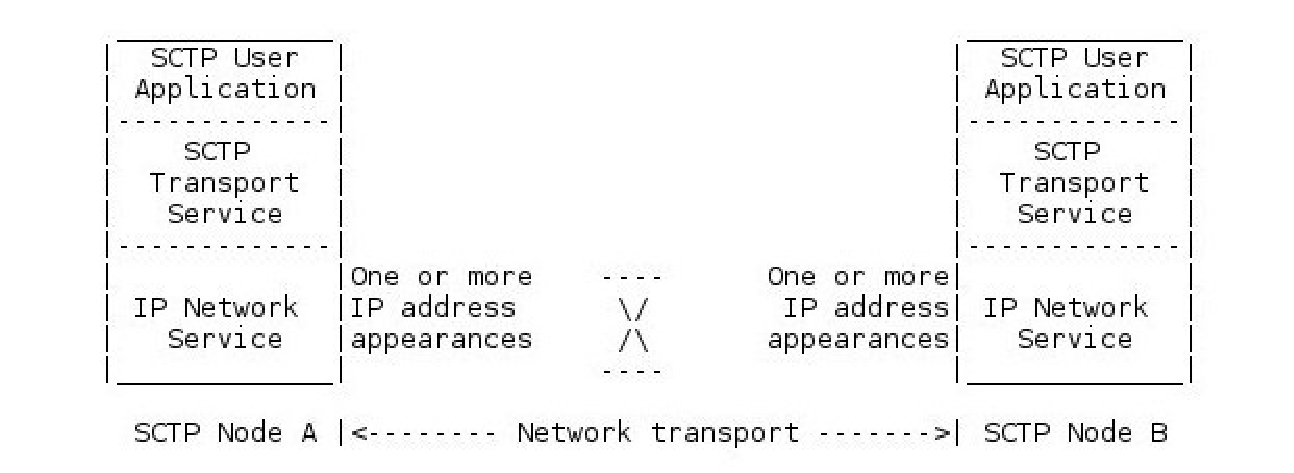
\includegraphics[scale=0.5]{images/sctp.pdf}
\caption{Overview of SCTP}
\end{figure}



\section{Summary}

In this chapter we have presented computer networks in general, before we
discussed the two most common types of Web services. Moreover, we have discussed
the protocols that these Web services use in order to transmit messages over the
Internet. We also introduced some new protocols designed to work in "Internet of
things" networks, which have many of the same characteristics as DIL networks.
The protocols are summarized in \cref{table:protocols:summary}. Finally, we
introduced the concept of performance testing and important network metrics when
doing such testing.

%%%%%%%%%%%% Transport protokoller %%%%%%%%%%%%%%%%%%%
\begin{table}[h]
\begin{tabularx}{\textwidth}{| l | l | X |}
\hline
  \textbf{Protocol} & \textbf{Network layer} & \textbf{Summary} \\ \hline
  TCP & Transport. & Stream-oriented transport protocol. Reliable and with congestion control. \\ \hline
  UDP & Transport. & Message oriented. Low overhead, but lacks reliability and TCP-friendliness. \\ \hline
  SCTP & Transport. & Similar to UDP but also provide reliable, in sequence transport of messages like TCP. \\ \hline
  HTTP & Application. Uses TCP. &  Widely used and the foundation for World Wide Web\\ \hline
  CoAP & Application. Uses UDP. & Low header overhead with optional reliability \\ \hline
  AMQP & Application. Uses TCP. &  Messaging middleware with store-and-forward capabilities.\\ \hline
  MQTT & Application. Uses TCP & Light weight and simple pub/sub protocol. \\ \hline
\end{tabularx}
\caption{Summary of protocols}
\label{table:protocols:summary}
\end{table}

Many of the mentioned protocols has been previously researched for use in DIL
networks. In the next chapter we will present relevant work in this area.

\chapter{Related Work}
\label{chapter:related-work}


In this chapter, we discuss earlier relevant work in the area of improving the
performance of Web services in \gls{dil} environments. Improving Web services is
important for both civil and military users as increasing the performance means
that applications can become faster and more reliable.

In the following sections, we identify studies and recommendations that apply to
this thesis. We get started by looking into the work of the NATO research groups
IST-090 and "SOA Recommendations for Disadvantaged Grids in the Tactical Domain"
(IST-118). IST-118 is an ongoing follow-on to the work of IST-090, with the goal
of creating a recommendation for a tactical profile for using SOA in
disadvantaged grids. Next, based on these recommendations, we investigate work
done in the area of alternative transport protocols and existing proxy
implementations.  Finally, we summarize the findings that are applicable with
regards to the scope and premises of this thesis.

\section{Making SOA Applicable at the Tactical Level}

IST-118 has published a paper\cite{ist-118} where they summarized the findings
of IST-090. Although the paper only looked into W3C Web services, many of their
recommendations are also applicable to RESTful Web services. They identified
three key issues that need to be addressed to adopt Web services in tactical
networks:

\label{section:DIL-problems}

\subsubsection{1. End-to-end Connections}

Web services mostly use transport protocols that depend on a direct, end-to-end
connection between a client and the service. Attempting to establish and
maintaining a connection in a DIL environment can lead to increased communication
overhead and the possible complete breakdown of communication. Most Web services use
TCP as their transport protocol, which relies on an uninterrupted connection.
In DIL environments with high error rates and high latencies,
the congestion control of TCP can cause sub-optimal utilization of the network
as previously discussed in \cref{section:tcp-problems}. Similar, HTTP, which is
the application layer protocol most often used together with TCP, struggles in
such environments. HTTP is a synchronous protocol, which means that the HTTP
connection is kept open until a response is received. Long response times could cause
timeouts. IST-090 points out the possible solution of replacing HTTP and TCP with
other, more suitable protocols.

The IST-90 report mentions two approaches to replace HTTP/TCP. The clients and
services themselves can be modified to support other protocols, or proxies
which support alternative protocols can be used \cite{ist-090}. Moreover, they
pointed out that if using a proxy approach, standards compliance can be
retained.


\subsubsection{2. Network Heterogeneity}

Another issue is when heterogeneous networks are interconnected. Different
performance in networks may lead to the buildup of data in buffers, risking the
loss of information. A proposed solution to this is to have store-and-forward
support which can support that messages are not dropped, but rather stored and
forwarded when possible. Another important usage of this technique is to
overcome network disruptions because messages can be stored until the network
connection is reestablished.


\subsubsection{3. Web Service Overhead}

W3C Web services are associated with a considerable amount of overhead. Web
Service technology is based on SOAP, which uses XML-based messages. It is a
textual data format and produces much larger messages than binary formats.
Optimization approaches should seek to reduce the network traffic generated by
Web services by using techniques as compression to reduce the size of messages.
Another method is to decrease the number of messages being sent, which was
looked into in IST-090 \cite{ist-090}. In their work they investigated three
different ways to do this:

\begin{enumerate}
    \item Employing caching near the client in order to reuse older messages.
    \item Using the publish-subscribe paradigm, which allows clients to subscribe to
    information instead of requesting it. This allows the same message to be sent
    to multiple clients.
    \item Employing content filtering which filters out unnecessary data.
\end{enumerate}

The scope of this thesis is to optimize for request-response type of clients and
Web services. Furthermore, since we are investigating general-purpose
optimization techniques without knowledge of the payload, some of these
recommendations does not quite apply to us. However, to reduce Web service
overhead, we can apply the well-known technique of compression.

\subsubsection{Compression}

Data compression is the technique of encoding information using fewer bits than
the original representation. In a network with limited data rate, the reduction
could significantly reduce time used to send the data. The reduction of data is
often expressed in the term \textit{compression rate}, which represents the
ratio between the uncompressed size and compressed size of the payload.
Moreover, there exist two types of compression, \textit{lossy} and
\textit{lossless compression}. Lossy compression is used to compress data such
as images and movies where the consequence of losing some of the data is not
critical. Lossless compression utilizes repeating patterns in the data in order
to represents the same information in a more efficient way.

\gls{xml} is the data format used by W3C Web services and has a significant
overhead. A previous study evaluated different lossless compressions techniques
for exchanging XML documents using W3C Web services \cite{johnsen-compression}.
They evaluated both XML-specific and general purpose (payload agnostic)
compression techniques. There exist a great number of different compression
techniques, so the authors focused on a few they saw as promising for use in
tactical communication networks. The first one, \gls{efx}, encodes XML documents
in a binary instead of textual format. The two other were the XML-specific XMLPPM
and general-purpose compression tool GZIP.

In their evaluation, they saw that for all techniques, larger XML documents
achieved a higher compression ratio than smaller documents. As the average, EFX
applied with a built-in proprietary ZIP enabled had the highest compression
ratio followed by GZIP. However, they concluded that all evaluated techniques
provided a significant reduction of payload size, so the specific technique was
of less importance.


\section{Previous Evaluations of Alternative Protocols}

A previous study has investigated potential gains from replacing HTTP/TCP with
alternative protocols \cite{evaluation-transport-protocols-web-services}.
\Citeauthor{evaluation-transport-protocols-web-services} looked into TCP, UDP,
SCTP and AMQP for conveying Web service traffic under typical military
networking conditions. The researchers found that \gls{sctp} had the highest
success rate in military tactical communication. However, on links with the
lowest data rate, the protocol tended to generate more overhead than TCP. They
pointed out that this was due to SCTP having a more complex connection handshake
procedure and besides using heartbeat packets.

Another study has compared the performance of MQTT and \gls{coap} concerning
end-to-end delay and network usage \cite{thangavel-mqtt-coap}.
\Citeauthor{thangavel-mqtt-coap} performed experiments in different emulated
networks with varying message sizes and loss rates. They saw that both MQTT and
CoAP were successfully able to handle packet losses of up to 25 \%. With lower
loss rates, messages sent with MQTT had the least delay, but as the loss rate
increased, CoAP had a lower delay. They identified the reason for this being
that the TCP transmission of MQTT had a larger overhead than CoAP's UDP
transmission. In their experiments with small message sizes and for all tested
loss rates, CoAP had less network overhead than MQTT. However, when the message
size grew, MQTT had less overhead than CoAP.

Another comparison of CoAP and MQTT was done in a study using the protocols for
sensor applications running on a smartphone \cite{caro-mqtt-coap}. This study
also confirmed CoAP as having lower network usage and a lower RTT. However, the
study pointed out that MQTT has more advanced \gls{qos} services, since it can
guarantee exactly-once delivery of messages. Since CoAP does not have this
feature, applications which require this functionality should consider using
MQTT.

CoAP has also been compared against HTTP in work done by
\citeauthor{walter-coap-http}, where they performed an evaluation with regards
to response time and energy consumption by a sensor node
\cite{walter-coap-http}. They found that using CoAP consumed significantly lower
energy than using HTTP and that CoAP also had  a lower response time.

\section{Proxy Optimization}

One of the recommendations of IST-090 was the usage of proxies. This
recommendation has been picked-up by other research groups and a set of proxies
for optimizing Web services in DIL networks already exist. However, many of them
do not fulfill all the requirements we have for our proxy. Some of them do only
support SOAP Web services, and others are unusable due to security reasons. This
section lists and discusses previous implementations of such proxies.

\subsection{Types of Proxies}

A proxy is a node deployed somewhere in a network, which through network traffic
can pass. Proxies have many use cases such caching, firewalling and security. To
adopt Web services into tactical networks, we mainly talk about two types of
proxies. Edge proxies act as gateways between different networks as illustrated
in \cref{figure:edge} and can perform adaptations on network traffic passing
through it.

\begin{figure}[h]
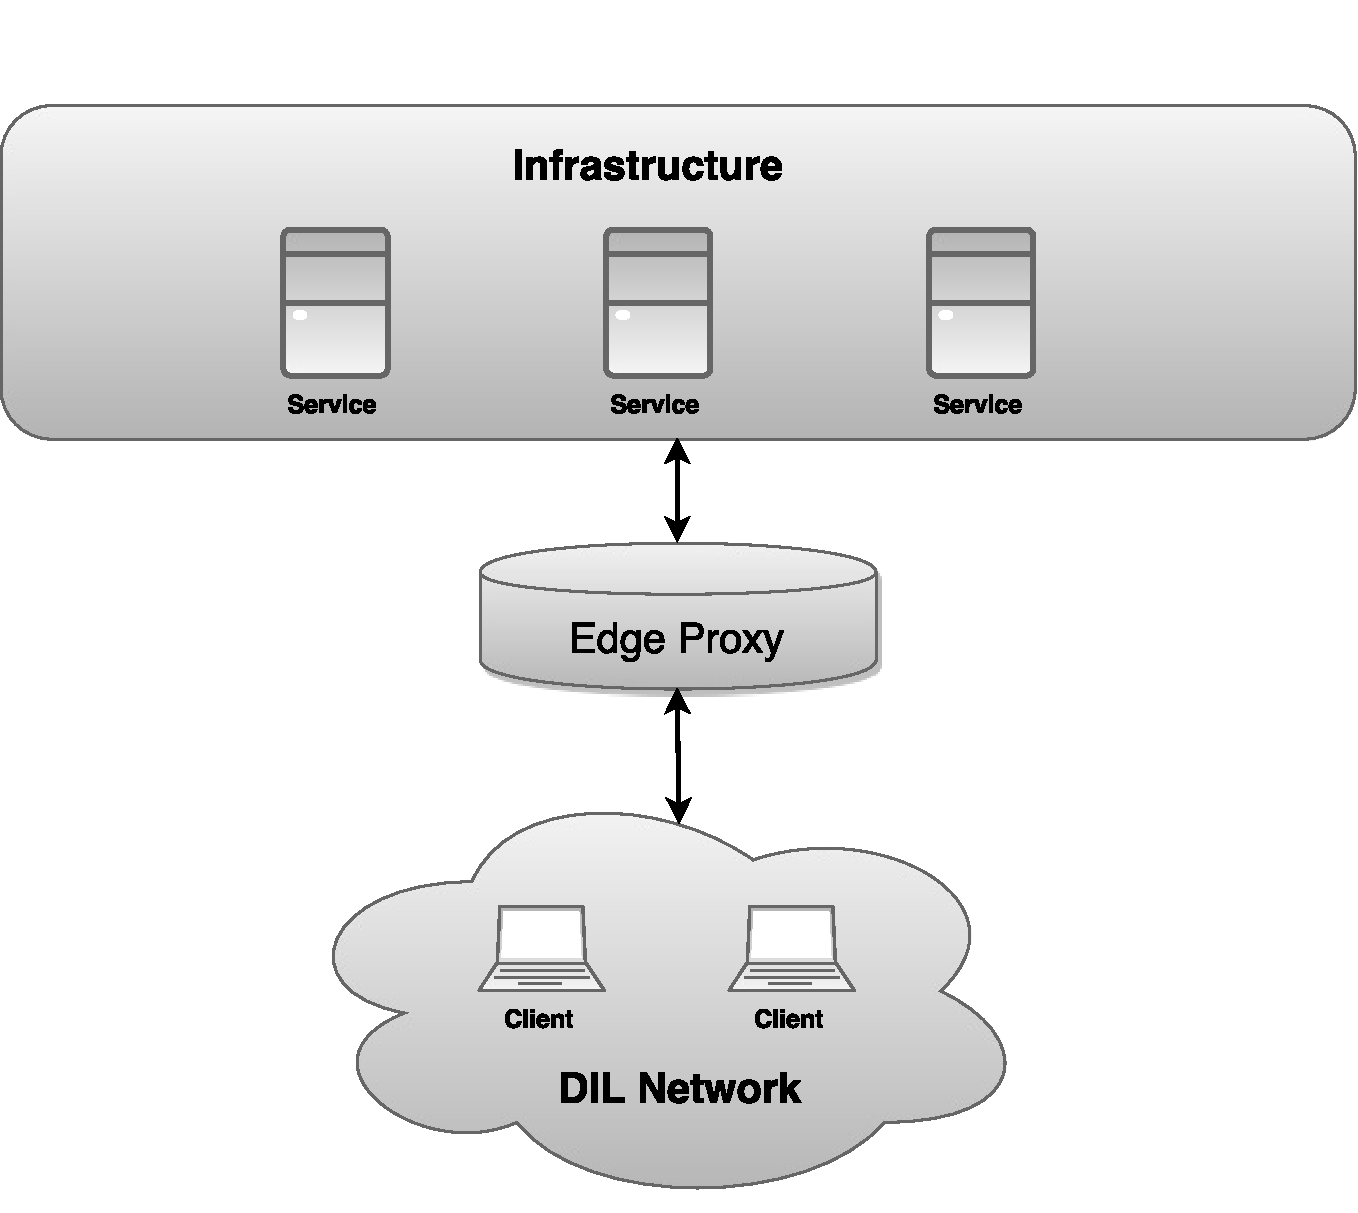
\includegraphics[scale=0.35]{images/edge_proxy.pdf}
\caption{Edge proxy}
\label{figure:edge}
\end{figure}

Another type, is point-to-point proxies in a network as illustrated in
\cref{figure:proxy-point}, which involves using a proxy-pair to facilitate
communication between two or more applications.

\begin{figure}[h]
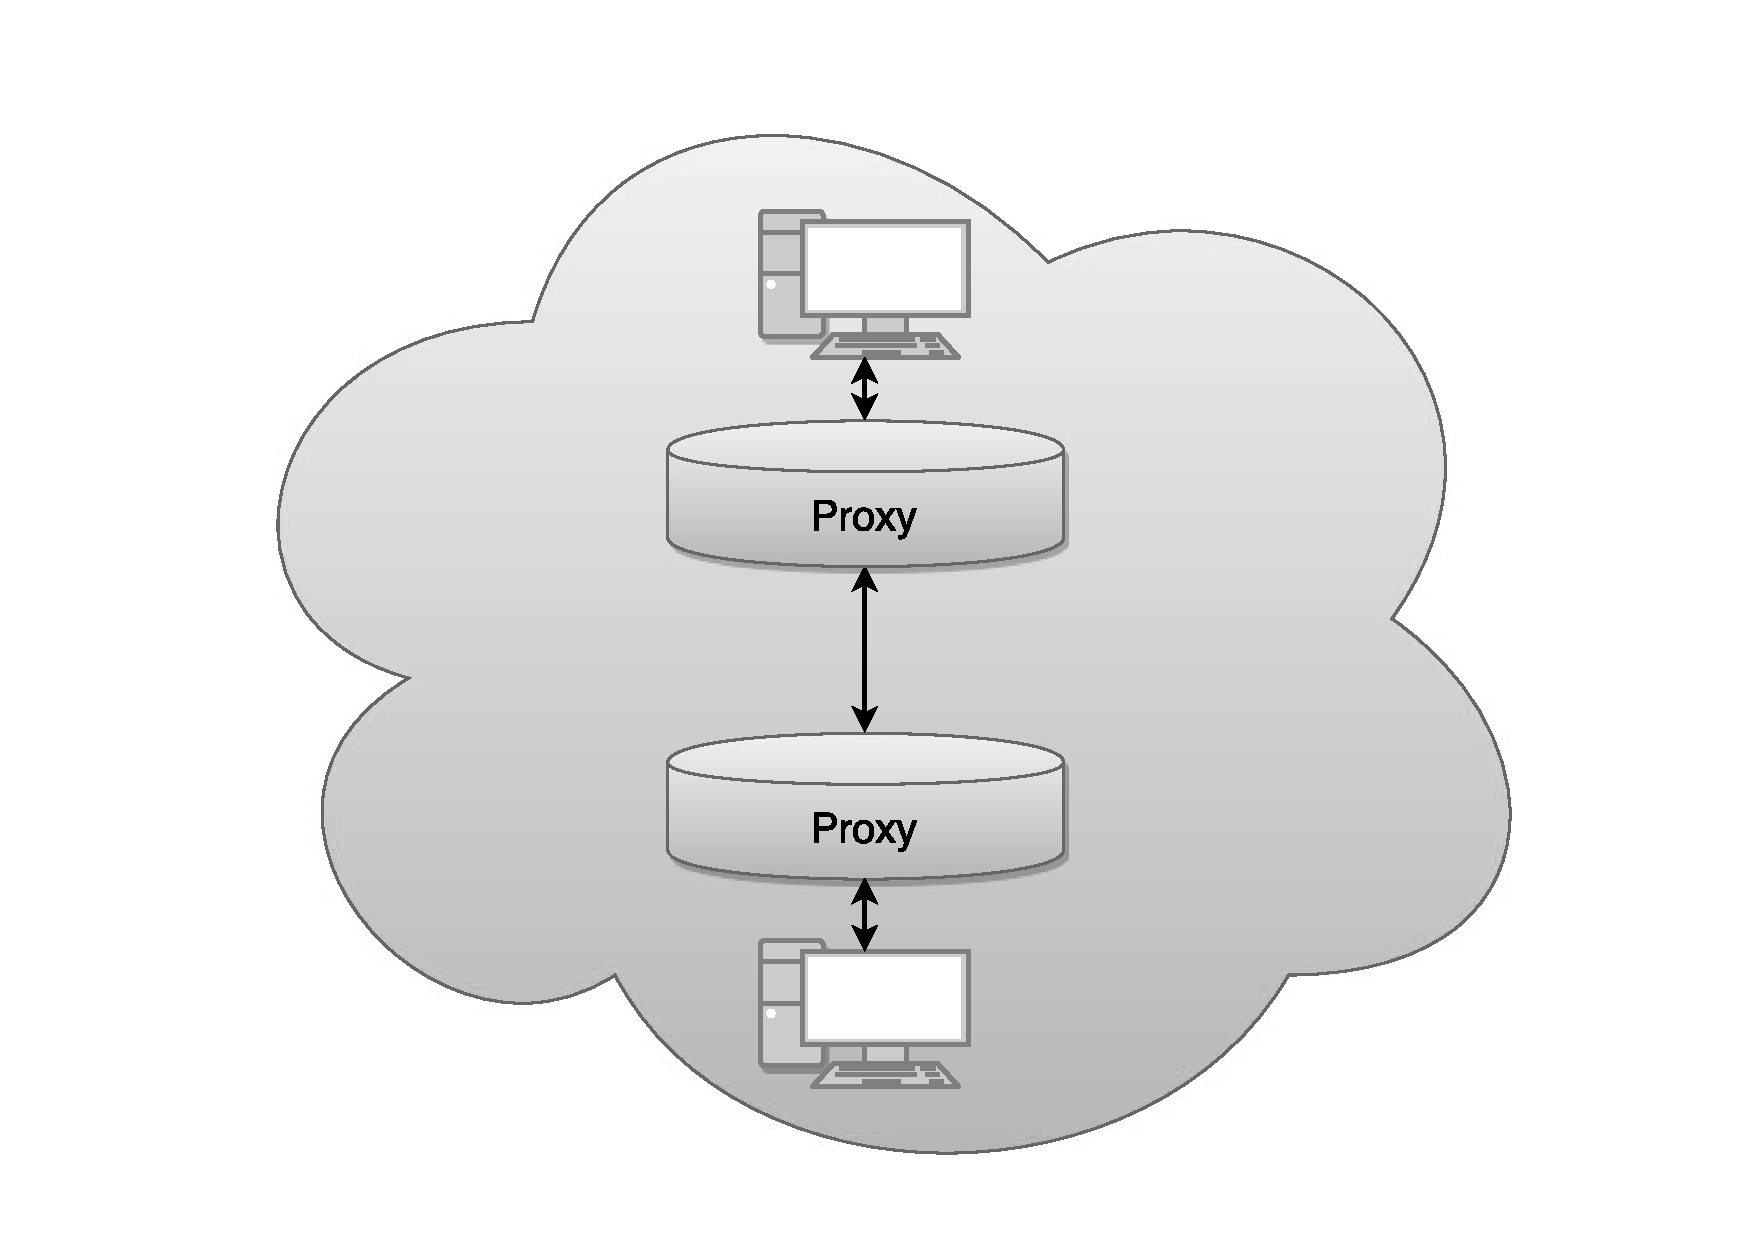
\includegraphics[scale=0.35]{images/proxy_point_gray.pdf}
\caption{Point-to-point proxy}
\label{figure:proxy-point}
\end{figure}

\subsection{\glsentrylong{dsproxy}}

The \gls{dsproxy} is a point-to-point proxy solution developed by \gls{ffi}
\cite{dsproxy-ffi}\cite{ieee-dsproxy}. Its goal is to enable the usage of
unmodified standard W3C Web services (SOAP over HTTP/TCP) in DIL environments.
The concept is to route all SOAP messages through the proxy. When the proxy
receive a message, it is stored locally before it is forwarded. If the
forwarding fails for some reason, it retries the request until it eventually
succeeds. This ability, called \textit{store-and-forward}, is one of the
fundamental core functionalities of \gls{dsproxy}. When a request eventually
succeeds, the response is returned to the client on the original TCP connection
initiated by a client. By doing this, Web service invocations is made possible
over unreliable networks by hiding any network disruptions from the client.

\begin{figure}[h]
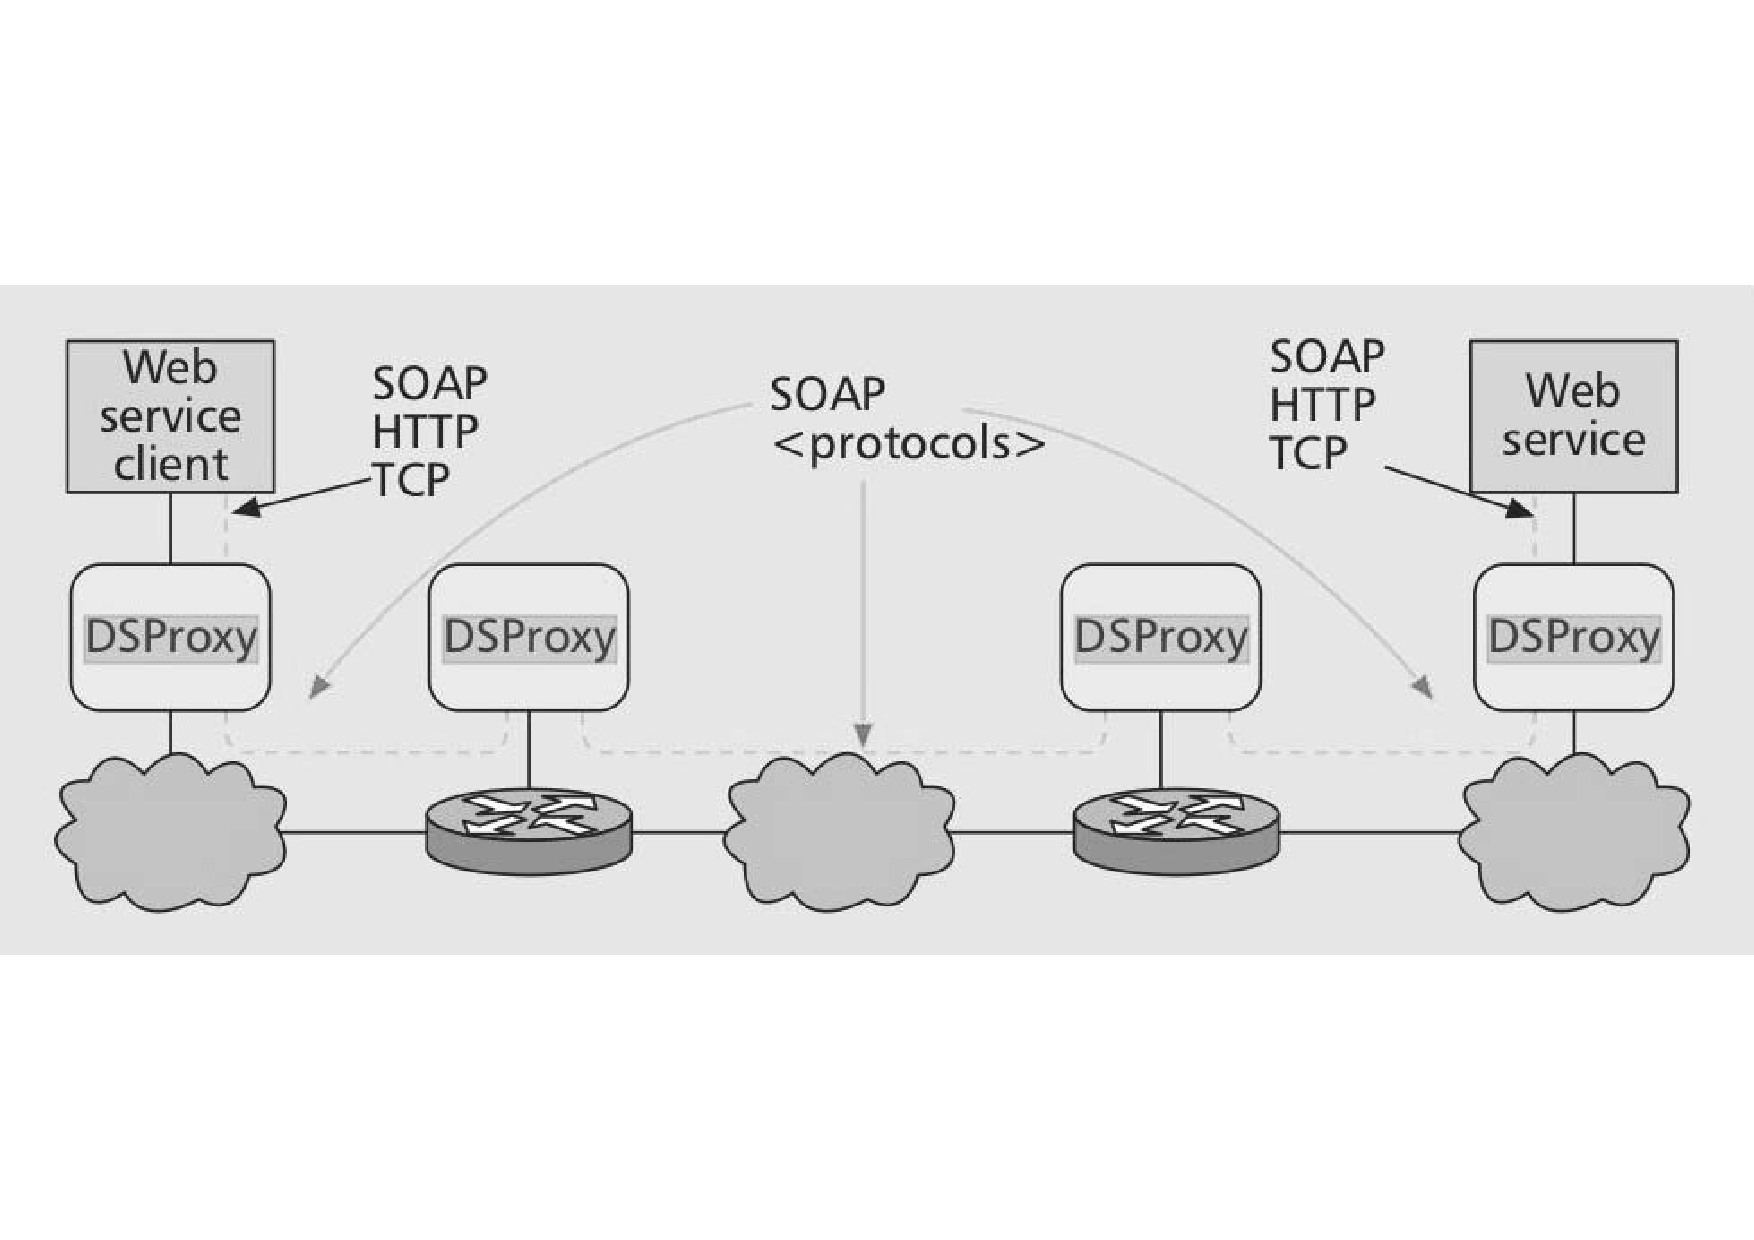
\includegraphics[scale=0.35]{images/dsproxy_gray.pdf}
\caption{DSProxy overlay network (from \cite{ieee-dsproxy} )}
\label{figure:dsproxy}
\end{figure}

Another core functionality of DSProxy is mechanisms for organizing an overlay
network consisting of multiple proxy instances as seen in \cref{figure:dsproxy}.
The overlay network enabled the ability to traverse multiple and heterogeneous
networks, but also add a lot of complexity to the proxy application. Apart from
the mentioned core functionalities, DSProxy support a set of pluggable
features such as GZIP compression and caching.

After performing experiments using the DSProxy, the researchers identified the
store-and-forward ability as important in unreliable networks to avoid having to
re-establish end-to-end connections each time the network connections was lost
\cite{dsproxy-ffi}. One of the downsides with DSProxy was that it only supported
W3C Web services. Moreover, it became very complicated due to its mechanisms for
building overlay networks and supporting different configurations and plugins.

\subsection{NetProxy}
%https://www.researchgate.net/profile/Niranjan_Suri/publications

NetProxy is another point-to-point proxy solution aiming at enabling SOA
applications for use in DIL environments \cite{suri-netproxy}. The proxy is a
component of the \gls{acm}, a set of components that satisfy many of the
communications requirements found in challenged networks. The work is being
carried out by researchers at the Florida Institute for Human \& Machine
Cognition.

Like DSProxy, NetProxy is a transparent proxy providing integration between SOA
systems without requiring modification of applications themselves. It works by
first intercepting all network traffic from applications and then do an analysis
of it. Together with information about the network, NetProxy then decides which
appropriate action to take. It can be configured to support protocol remapping
by using other protocols than HTTP/TCP. Integrated with NetProxy is the
message-oriented transport protocol \gls{mockets}, which is designed to replace
\gls{tcp} and \gls{udp} and is targeted for DIL networks \cite{suri-netproxy}.
Mockets substitutes the congestion control and reliable transmission algorithms
of TCP with other alternate implementations designed for DIL networks. It is
configurable for different types of networks and offers various \gls{qos}
levels.

Performance testing of W3C Web services showed that using NetProxy with Mockets as
the transport protocol yielded a significant increase in the performance
compared to plain TCP \cite{suri-netproxy}. The researcher attributed this to
several factors:

\begin{itemize}

    \item Mockets handles packet loss much better than TCP since TCP attributes
    packet loss to congestion and triggers its congestion control.

    \item NetProxy multiplexes all network traffic directed to a single node
    onto the same connection and holds it open instead of closing it after a
    finishing request. This allows reusing the connections across consecutive
    requests, also from other applications.

    \item Less overhead due to the fact that NetProxy buffers data until it fills an
    entire packet before sending it over the network.

    \item Enabling compression gave a very high gain in the measured network
    throughput partly due to the messages subject for compression was XML
    documents, which have a relatively high compression rate.

\end{itemize}

Although the testing shows some promising results, there are some issues
regarding using the Mockets protocol in our proxy solution. Applications meant
for usage in military systems, must be approved by military security
authorities. Mockets has not been standardized and lacks usage outside the
experiments conducted in the mentioned research. Because of this, it may be
difficult to get applications using Mockets approved.

\subsection{AFRO}

\gls{afro} is an edge proxy which offers different levels of \gls{qos} to Web
services through performance monitoring and usage of the context-aware service
provision paradigm \cite{ist-090}. It performs so-called adaption actions, which
modifies the SOAP XML messages by changing their encoding to more efficient data
representation. \gls{afro} also removes information that is acceptable to be
removed by the service requester.

However, since the proxy modifies the data being sent, the digital signature of
the data is also changed. In applications where we want to be sure that no one
has tampered with the data before arriving, digital signatures are often used.
Consequently, this solution would not work for such applications.


\subsection{TACTICS TSI Architecture}

Another ongoing effort to overcome issues using standard Web services in
tactical networks is the TACTICS project supported by the \gls{eda}
\cite{tactics-diefenbach}. The goal of the project is to propose a reference
architecture for a \gls{tsi} suited for establishing a tactical \gls{soa} of
defence-related information systems. The architecture features a service
middleware meant to run on devices with different capabilities. The purpose of
the middleware is to receive standard Web service invocations or responses and
ensure that they complete. The middleware can forward IP packets between
different radio networks and store and forward messages. The concept is based on
the point-to-point proxy approach.


\section{Tuning Application Server Parameters}

 Another approach to improve the performance of Web services is to configure
 the way they are deployed. Web services can be deployed in applications
 servers, which is a software framework that provides an environment where the
 Web services can run. When setting up an application server, several parameters
 which can affect the performance of running applications can be
 configured. A wrong or bad configuration may cause inaccurate timeouts and
 congestion in the network. In a paper written by researchers at \gls{ntnu} and
 FFI \cite{johnsen-recommendations}, they
 investigated how tuning the server parameters of the application server
 Glassfish affected the performance of both \gls{rest} and SOAP Web services.
 They identified a number of key HTTP and TCP tuning parameters:

\paragraph{HTTP Timeout} Controls how long a HTTP connection can be deemed as
idle and kept in the "keep-alive" state. Having a too low timeout on networks
with low data rate, can potentially flood the network with packets that have
timed out. Consideration should therefore be taken when setting this
parameter for mobile tactical networks.

\paragraph{HTTP Compression} Enables HTTP/1.1 GZIP compression.

\paragraph{HTTP Chunking} Allows the server to send data in dynamic chunks.

\paragraph{HTTP Header and Send Buffer Sizes} Vary the size of the buffers
that hold the request and send the data.

\paragraph{TCP Idle Key Timeout} Sets the time before an idle TCP channel
closes.

\paragraph{TCP Read and Write Timeouts} Set the timeout for TCP read and write
operations, respectively.

\paragraph{TCP Selector Poll Timeout} Sets the time a \gls{nio} selector will
block waiting for user requests.

\paragraph{TCP Buffer Size} Sets the size of the buffer that holds input streams
created by the network listener.

\paragraph{TCP Batching/TCP NO\_DELAY} Batches together small TCP packets into
larger packets.

\paragraph{MTU Size} The maximum transmission unit size regulates the largest
data unit that can be passed onwards. In tactical military communication the MTU
size can be very low (down to 128 bytes).

\paragraph{}

After running their experiments, they concluded that few of the parameters
actually had any significant impact on the performance of the Web Service.
However, they identified HTTP Chunking configuration as having the most impact
on the performance. It significantly improved the performance for both SOAP and
RESTful Web services in different types of networks.

While tuning application server parameters may help improve the performance of
Web services in DIL environments, it is not directly related to the proxy
solution investigated in this thesis. When deploying Web services, this
optimization technique should be considered, but are not explored further in
this thesis.


\section{Summary}

In this chapter, we looked into efforts previously undertaken in order to
improve the performance of Web services in networks with the DIL
characteristics. We first investigated the work of the research groups IST-090
and IST-118, and saw how they identified end-to-end connections and Web service
overhead as major issues for enabling Web services in DIL environments. To
overcome these problems, they recommended the usage of proxies and several
techniques for reducing the overhead. We identified GZIP and EFX with zipping as
important compression techniques to reduce the size of Web service messages sent
over a network. Next, we looked into previously developed proxies for DIL
networks. Although many of them showed promising results, some of their
properties did not fulfill the premises for this thesis. They were either
limited to SOAP-based Web services or are inadequate to be used due to security
reasons. However, we identified some of their techniques that we carry on in the
proxy developed in this thesis.

Finally, we investigated previous attempts with the usage of alternative
transport protocols, before we looked into previous efforts in the area of
tuning application server parameters. Based on recommendations and studies of
previous work, we are in the next chapter deriving a set of requirements for our
proxy.

\chapter{Requirement Analysis}
\label{chapter:requirements}

In this chapter we discuss the requirements for optimization techniques aiming
at enabling Web services in DIL environments. These requirements build on the
scope and premises discussed in the introduction. To recap, the defining
premises were that the proxy should:

\begin{enumerate}
    \item Support HTTP RESTful and W3C Web services.
    \item Work in DIL networks.
    \item Be interoperable with standards-based COTS solutions.
    \item Work with security mechanisms.
\end{enumerate}

Based on previous research, in particular the work of the \gls{nato} research
groups IST-090 and IST-118, we are in thesis developing a proxy solution
supporting these premises. In the following sections we discuss the specific
requirements for this approach.

\section{HTTP Proxy}

The first premise implies that our proxy must accept \gls{http}, as this is the
far most used Web service transport protocol. Furthermore, the third and fourth
premises have some important implications for our proxy. Our proxy must be able
to accept HTTP requests from a Web service, forward it to the other proxy, which
in turn delivers it to the intended receiver. The communication between the
proxies is not required to be with HTTP, but rather using a protocol that deals
with DIL networks in a better way. However, since ultimately a HTTP request
should be delivered to the intended receiver, the HTTP properties must be
retained. This means that the proxy must preserve the HTTP method and headers.
Also, since REST is payload agnostic, the proxy must be able to support
different types of data being sent through it (XML, JSON etc.).

Furthermore, the proxy must be able to handle the difficult network conditions
of DIL. The specific requirements are outlined in the following sections.

\section{Cope with DIL Networks}

The \gls{dil} term refers to three aspects of a network, \textit{disconnected,
intermittent} and \textit{limited}. The proxy should be able to
overcome the implications of these aspects. In the following sections we discuss
the requirements each aspect implies.

\subsection{Disconnected}

The Disconnected aspect of DIL refers to disconnects for a longer period of
time. As we saw in the previous chapter, earlier work has identified the removal
of end-to-end dependencies as important to overcome this aspect. Without
proxies, a disconnect for a longer period of time would cause a timeout
exception at the Web service, leaving it up to Web service itself to deal with
the exception. By employing a proxy pair, the end-to-end dependency is instead
moved from between a client and a Web service, and to between the client and the
locally deployed proxy. As a result, the connection between the proxies over a
DIL network can be lost, while still maintaining the connection between the
client and local proxy. When the connection is reestablished, the proxy must be
able to continue transmission of messages on behalf of clients.

This requires the proxy to have some sort of redelivery mechanism. When a proxy
detects that it unable to transmit messages to the other proxy, it should
ideally wait until the connection is reestablished before trying to send more
messages. However, the only way to know if the connection is reestablished is to
try and send more messages and see if they succeed. The first, and maybe naive
approach, could be to just retransmit the message again and again. But by doing
this, we could risk overflowing a slow receiver, as well as causing congestion
in a possibly overloaded network. Different types of networks and different use
cases for the applications involved may require different redelivery mechanisms.
At deployment, the proxy should therefore support a  set of configurable
redelivery mechanism properties:

\begin{description}

    \item[Redelivery Delay] The proxy should support the retransmission of
    sending messages with a fixed delay between each attempt.

    \item[Exponential Backoff] If exponential backoff is configured, the proxy
    should gradually try resending more and more seldom.

    \item[Maximum Redeliveries] The proxy should support user configuration of
    how many times a retransmission should be attempted before giving up.

\end{description}


\subsection{Intermittent}

The proxy should handle brief, temporary disconnects that can occur in a DIL
network. It is comparable to the disconnect aspect, as intermittent refers to a
shorter disconnect. A "long" intermittent disconnect triggers a timeout at the
application layer and should be dealt with by the proxy retransmission
mechanisms. With shorter intermittent disconnects, the transport protocol should
be able to deal with it. This requires using a reliable transport protocol, or
handling it in the application layer.

\subsection{Limited}

Limited refers to different ways a network can be limited. Accordingly, the
proxy must cope with very low data rates, possible high error rates and long
delays. This implies that reducing Web service overhead in order to lower the
amount of bytes that need to be sent over a limited network is important.
Moreover, the proxy may run on machines with restricted resources (battery
capacity), which means that a low CPU overhead is desired.

\section{Support Optimization Techniques}

To improve the performance of Web services in DIL environments, the proxy should
support a set of optimization techniques. As we discussed in the related works
chapter, there exist many approaches to optimizing Web services. Reducing Web
service overhead by using compression was identified as a technique that yields
a significant improvement. Another approach was the usage of alternative
transport protocols. In this thesis we focus on compression and the usage of
alternative protocols as the means of optimizing Web services.

\subsection{Compression}

Compression reduces the size of a message sent over a network. In order to
perform compression the proxy must be able to modify the payload of the message.
Due to security mechanisms that detect changes to the payload (digital
signatures), the payload must be restored back to its original form before being
forwarded to the final receiver. One of our premises is that we must support
both RESTful and W3C Web services. RESTful services do not put any restrictions
on the data format of a message. Thus, we cannot use XML-specific compression,
but rather we need to use general-purpose techniques.

Based on previous work we identify GZIP as the best approach for general
purpose compression.

\subsection{Proxy Protocol Communication}

One of the optimization techniques we identified is the usage of alternative
transport protocols between the proxy pair. We introduced a set of protocols in
the technical background chapter and discussed previous evaluations using them
in DIL networks in last chapter. In the following paragraphs we analyze them for
usage in the context of proxy communication in a DIL network.

\begin{description}

    \item[\gls{http}] The by far most used protocol for Web services is HTTP
    over TCP. TCP is an old and proven protocol and was originally designed to
    provide reliable end-to-end communication over unreliable networks. The
    less intrusive optimization technique would therefore be that the proxies
    simply forward HTTP-requests without using an alternative protocol.
    Although proxing Web service requests through proxies would cause some overhead from
    processing time and custom proxy headers, we still get the benefit of
    breaking the end-to-end dependency and the possibility of using compression.
    Furthermore, using HTTP allows us to compare the "standard" protocol against
    other protocols. We therefore recommend HTTP as a possible proxy pair
    communication method.

    \item[\gls{udp}] UDP has less overhead than TCP, but lacks mechanisms for
    reliability and congestion control. The lack of reliability could be handled
    at the application level instead, but would require a library on top of it.
    Furthermore, UDP is not TCP-friendly. For these reasons, we conclude that UDP
    is unfit for proxy communication as part of this thesis.

	\item[\gls{coap}] CoAP is a relatively new protocol intended for use in the
	Internet of Things. It is designed to have low overhead, low code footprint
	and be easily mapped to and from HTTP. These properties make the protocol
	very interesting as the means of communication between a proxy pair.

	\item[\gls{amqp}] AMQP is in widespread use and offers reliable message
	transmission. It supports both the request-response and publish-subscribe
	message paradigms. We therefore recommend AMQP as a possible proxy pair
	communication method.

	\item[MQTT] MQTT is a publish-subscribe messaging protocol and is considered
	as lightweight and simple to implement. However, the inter-proxy
	communication requires a request-response type of messaging. MQTT does not
	facilitate this type of communication. With that said, it is possible to
	have a request-response paradigm on top of publish-subscribe by organizing
	queues and by using some application logic. However, since MQTT does not
	natively support request-response, we do not recommend this protocol for
	proxy pair communication.

	\item[\gls{sctp}] SCTP offers functionality from both UDP and TCP. It is
	reliable and has been identified in previous related work as an interesting
	protocol for DIL networks. We therefore recommend it as a possible proxy
	communication method.

\end{description}

The proxy should support the identified protocols found suitable for
communication between proxies over a DIL network. The recommendations are
summarized in \cref{table:possible-proxy-protocols}. For evaluation purposes the
proxy should be easily configured of which protocol to use.

\begin{table}[h]
\begin{tabularx}{\textwidth}{| X | X |}
\hline
  \textbf{Protocol} & \textbf{Recommendation} \\ \hline
  HTTP & Yes \\ \hline
  UDP & No \\ \hline
  CoAP & Yes \\ \hline
  AMQP & Yes \\ \hline
  MQTT & No \\ \hline
  SCTP & Yes \\ \hline
\end{tabularx}
\caption{Protocols recommended as possible proxy communication protocol.}
\label{table:possible-proxy-protocols}
\end{table}



\section{Summary}
\label{section:requirements-summary}

In this chapter we have discussed the requirements for our proxy, which we
summarize here:

\begin{enumerate}
    \item Receive and forward HTTP requests.
    \item Retain HTTP request and response headers.
    \item Support GZIP compression of payload.
    \item Handle frequent network disruptions.
    \item Handle disconnects over longer periods of time.
    \item Handle low data rates, high delays and high packet error rates.
    \item Allow for configuration of redelivery delay and maximal number of retransmissions.
    \item Support usage of different transport protocols between the proxies.
    \item Easy configuration of which protocol to use.
    \item Be easily extendable to include other protocols and other optimization techniques.
\end{enumerate}

Next, we discuss the design and implementation of our proxy supporting the
premises and identified requirements.

\chapter{Design and Implementation}
\label{chapter:design}

Based on the requirements identified in the previous chapter, we're in this chapter introducing the design and implementation details of the of our proposed proxy solution. We get started by discussing the overall design, before we dive into the implementations details.



\section{Design of Solution}

In previous chapters we have argued that all optimization techniques should be
placed in proxies in order to retains interoperability for COTS applications, as
well as to break their end-to-end dependency. Our design therefore deploying a
proxy pair to facilitate Web communication. The idea is to deploy the proxy pair
in two different locations separated by a DIL network. Through the locally
deployed proxy can then Web applications proxy all their communication. The
proxy will then apply different optimization techniques, and over over a DIL
network forward the request to the other proxy, and finally return a response.
Ideally should a proxy be deployed as close to its intended user applications as
possible, preferable at the same machine.


It is worth noting that since the proxies is designed to accept \textit{all} HTTP
requests, they can support any applications that utilize HTTP, including request-
response and publish-subscribe applications.


\subsection{Design of HTTP proxy}

A deployed proxy is designed to accept arbitrary HTTP requests, possible from
multiple clients, and forward them to the other proxy as seen in
\cref{figure:proxy_design}. Ideally the proxy should be deployed as close to its
intended users as possible, as the communication between an application and its
proxy is not subject to any optimization for DIL environments.

\begin{figure}[h]
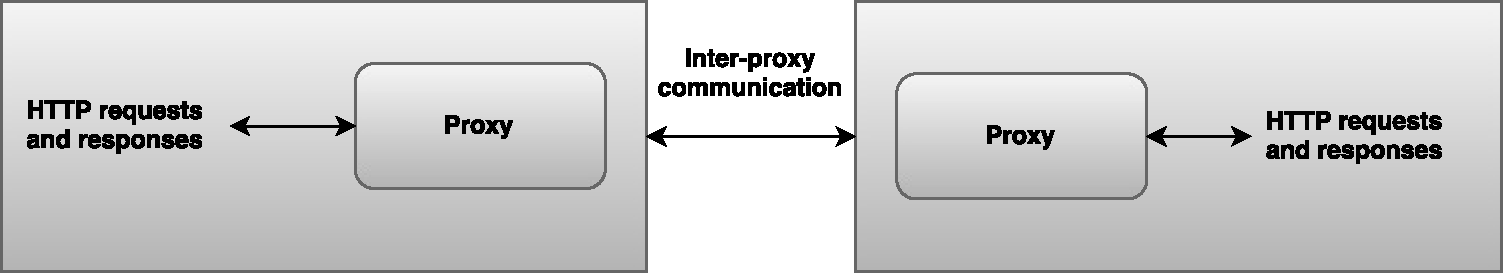
\includegraphics[scale=0.55]{images/proxy_design.pdf}
\caption{Design of Solution}
\label{figure:proxy_design}
\end{figure}

It is the communication between a proxy pair that is subject to optimizations.
The proxies are therefore designed to support the optimization techniques we
have identified. Those are primarily concerned about using different transport
protocols as the inter-proxy communication, as illustrated in
\cref{figure:proxy-communication}. The purpose of this is to evaluate the
performance of the transport protocols in DIL networks. Which protocol to use as
the means of inter-proxy communication is therefore designed to be easily
configured by the user of the proxy.

\begin{figure}[h]
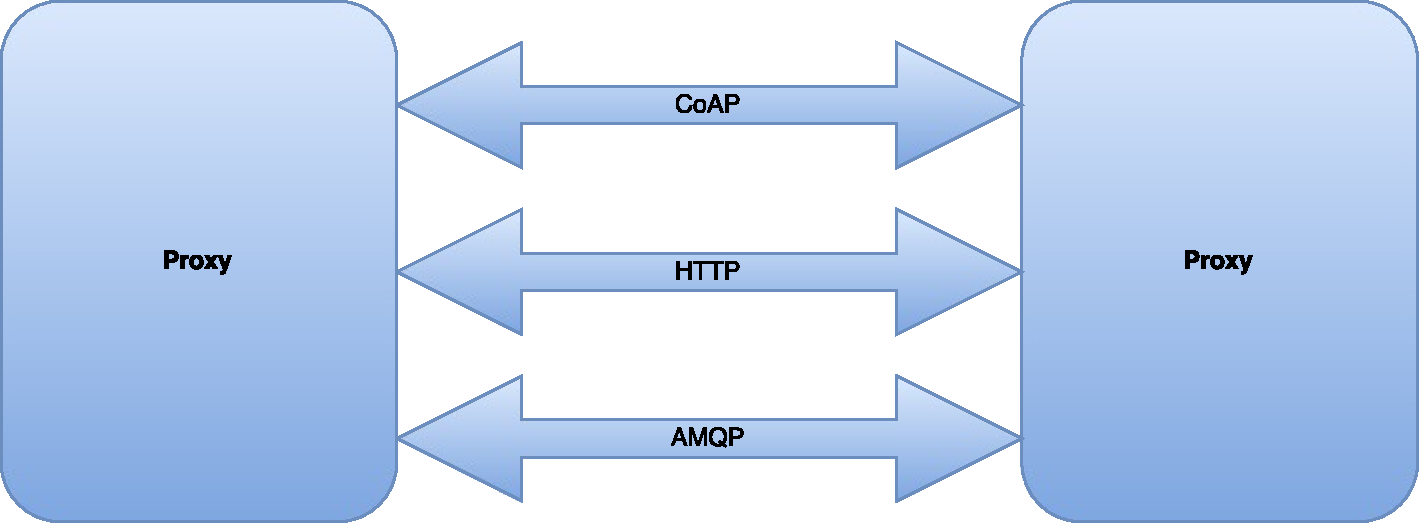
\includegraphics[scale=0.5]{images/proxy_communcation.pdf}
\caption{The proxies were designed to support multiple protocols for inter-proxy communication}
\label{figure:proxy-communication}
\end{figure}

\section{Choosing a Framework}

Requirement one implies creating a HTTP proxy which accepts HTTP requests,
forward them, and finally return a HTTP response. We identified some approaches:

\begin{enumerate}
    \item Build a HTTP proxy from scratch ourself.
    \item Use an existing HTTP proxy.
\end{enumerate}

Building a HTTP proxy ourself would allow us to customize our solutions as we
wanted, but would require a lot of implementation. We therefore concluded that
best use of our resources was to use an existing configurable proxy. Building on
state-of-art existing solutions allowing us to focus on the optimization
techniques, rather than on the specific low-level details of HTTP. There are
numerous HTTP proxies available for use, for an example Nginx and Squid.

Another one is Apache Camel, which is an open source Java framework developed by
the Apache Software Foundation for rule-based routing and
mediation\cite{camel-homepage}. It has a wide range of use-cases and focuses on
making integration between different enterprise communication system easier. It
support a large set of different communication transports (transport protocols).
We chose to use Apache Camel as our HTTP proxy due to its simplicity and support
for different transport protocols.

\subsection{Apache Camel}

Routing is a central concept in Apache Camel and consist of defining a
\textit{from route}. This is an endpoint from which Camel consumes messages. It
can then invoke a series of \textit{processors}, which can modify the headers,
payload etc. of the message. Then, Camel forwards the message to a \textit{to
route}, which can be an application running somewhere else. When a response is
received, Camel can invoke a new set of processors on the message, before it is
finally returned to the origin. An overview of this can be seen in
\cref{figure:camel-route}.

Describe Camel Components.

\begin{figure}[h]
\centering
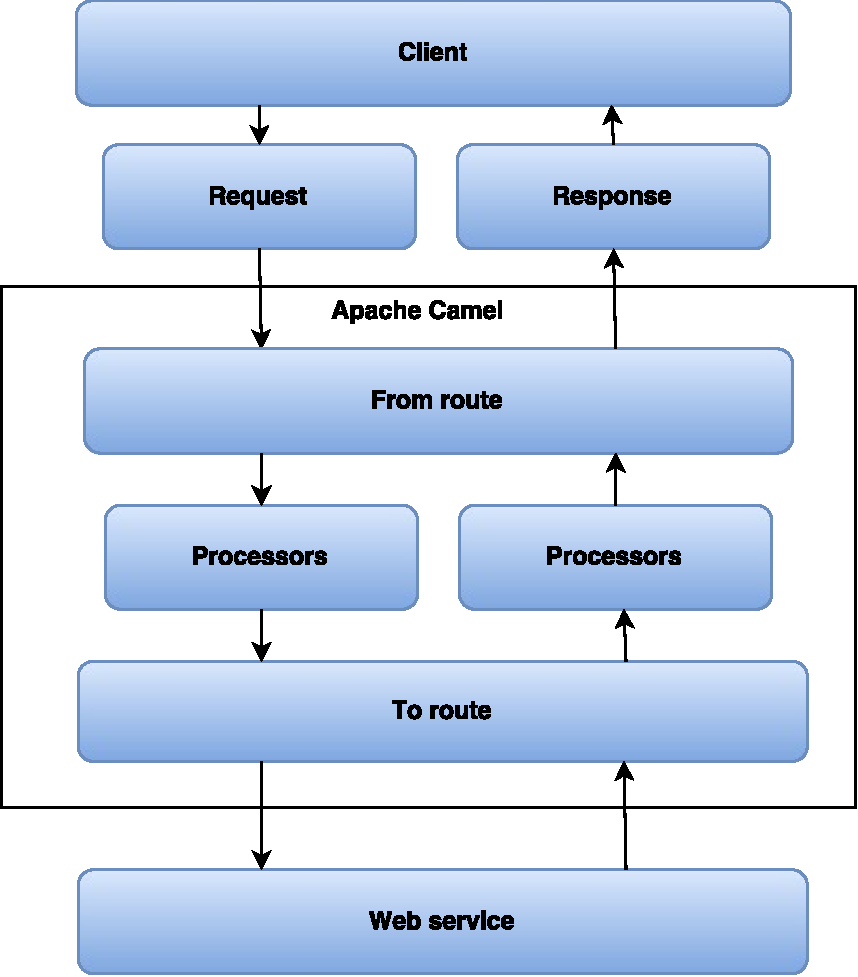
\includegraphics[scale=0.7]{images/camel_routes.pdf}
\caption{Example of a Camel route}
\label{figure:camel-route}
\end{figure}

\section{Implementation}

The proxy was implemented as a Java 1.8 application using the Apache Camel
framework. A large part of the implementation is concerned about reading user
configuration and setting up \textit{routing rules} for Apache camel. The stages
of the program are as follows:

\begin{enumerate}
    \item Reading and parsing user configuration.
    \item Initializing Camel components.
    \item Setting up routes.
    \item Running.
\end{enumerate}

\subsection{Parsing Configuration}

The first stage involves reading a user provided configuration file. Details about the configuration is explained in section X.

\subsection{Initializing Components}

Depending on which protocol the user has selected for usage as inter-proxy
communication, at startup the respective Camel component is initiated  and added
to the Camel context.

Due to the time available, we did not implement support for all of the
recommendation protocols from the last chapter. The currently supported protocols
are HTTP, AMQP and CoAP. However, the proxy is designed to by easily extended to
include additional protocols.

\subsubsection{HTTP Component}

We made use of the Camel component Jetty in order to consume and produce HTTP
requests. The component is based on the Jetty Web server\cite{jetty-homepage}.
It was used for two purposes: to consume \gls{http} requests from applications
and if HTTP was configured,as the selected protocol, to consume/produce HTTP
messages as part of the inter-proxy communication.

\subsubsection{AMQP Component}

Describe AMQP component.

\subsubsection{CoAP Component}

Describe CoAP component

\subsection{Routes}

A running proxy listens on two \textit{routes}. It can either receive messages
from an application, or it can receive a message from the other proxy. This
setup can be seen in \cref{figure:dil-routes}. The routing logic is different
for these two cases. We define a request origination from an outside application
as the \textit{application route}, and a request origination from another proxy
as a \textit{proxy route}. We discuss these routes, but first we need to
introduce what we have chose to call the \textit{proxy message format}.
Requirement 2 says that we need to retain all the original HTTP headers from the
original request. Consider if the proxy receives a HTTP request and forwards it
to the other protocol using AMQP. The message itself will arrive correctly, but
the original HTTP headers and method would be lost. Our approach to this was to
introduce a custom \textit{proxy message format}, which is discussed in the next
section.

\begin{figure}[h]
\centering
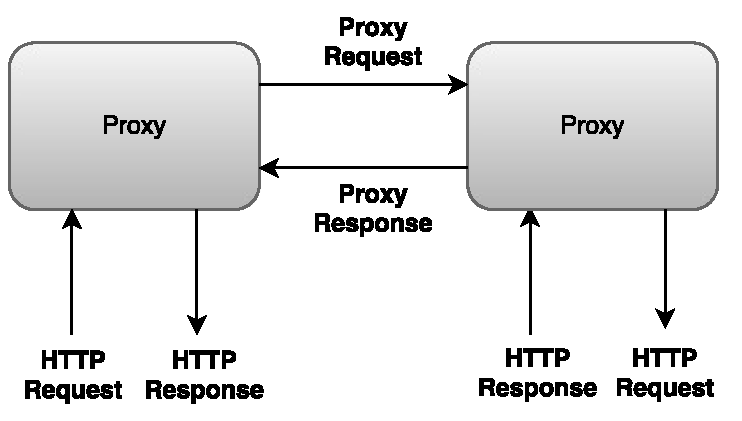
\includegraphics[scale=0.7]{images/dil_routes.pdf}
\caption{Proxy routes}
\label{figure:dil-routes}
\end{figure}

\subsection{Proxy Message Format}

The proxy message format was developed to retain HTTP headers and other
necessary information about the request. Our solution was to wrap all messages
in a \gls{json} document and include necessary information as properties in the
JSON document. JSON is a lightweight, text-based data format\cite{rfc-json}. We
chose this data format due to its compactness, simplicity and the wide support
for libraries for generating and parsing JSON. Due to a HTTP request and
response having slightly different semantics, we used the same format, but
with different properties for a request and response. The request format is
defined in \cref{table-proxy-request}, and the response format in
\cref{table-proxy-response}.

\begin{table}[h]
\begin{tabularx}{\textwidth}{|l|X|l|}
\hline
\textbf{Field} & \textbf{Purpose}                                                                                                      & \textbf{Required} \\ \hline
path           & The original request URL from the application. Specifies the intended final destination of the original HTTP request. & Yes               \\ \hline
method         & HTTP method of the request.                                                                                           & Yes               \\ \hline
query          & Query string associated with the original HTTP request.                                                               & No                \\ \hline
headers        & JSON object containing all the original HTTP headers of the request                                                   & Yes               \\ \hline
body           & The original payload of the message                                                                                   & No                \\ \hline
\end{tabularx}
\caption{Proxy message request fields}
\label{table-proxy-request}
\end{table}

\begin{table}[h]
\begin{tabularx}{\textwidth}{|l|X|l|}
\hline
\textbf{Field} & \textbf{Purpose}   & \textbf{Required} \\ \hline
headers        & JSON object containing the HTTP response headers. & Yes  \\ \hline
responsecode   & The HTTP response code. & Yes \\ \hline
body           & Response body of the HTTP request. & No            \\ \hline
\end{tabularx}
\caption{Proxy message response fields}
\label{table-proxy-response}

\end{table}

An example proxy request message is included in \cref{listing:proxy-request}.
The listing illustrates a HTTP request originating from an outside application.
It was a POST to the intended destination http://myservice.com, with a XML
message as payload.

\lstinputlisting[frame=single, language=json, firstnumber=1, caption="Example proxy request", label=listing:proxy-request]{listings/proxy_message.json}

\paragraph{}

\subsection{Application Route}

The purpose of the application route is to consume HTTP requests from an
outside HTTP request, transform it to a proxy request message and deliver it
to the other proxy. When a response is received, return it to the application.
The route consist of the following steps:

\begin{enumerate}
	\item Defining a HTTP endpoint to consume HTTP requests from. This is read from the configuration which specifies which hostname and port to listen on.
	\item Consume HTTP request from an outside application
	\item Apply the \textit{ProxyRequestPreProcessor}. This processor converts the message into a Proxy Request Message.
	\item If compression is enabled, compress the entire message.
	\item Forward the request to the other proxy using the configured transport protocol.
	\item Receive an response from the other proxy.
	\item If compression is enabled, de-compress the message.
	\item Restore the HTTP response from Proxy Response Message.
	\item Return the response to the application.
\end{enumerate}

\subsection{Proxy Route}

The purpose of the proxy route is to listen for messages from the other proxy,
de-serialize it, and deliver it to its intended receiver. When a response is
received, transform it into a Proxy Response Message and return it to the other
proxy. The route consist of the following steps:

\begin{enumerate}
	\item Defining a endpoint depending on which the configured protocol.
	\item Consume requests from the other proxy.
	\item If compression is enabled, de-compress the message.
	\item Transform the message into the original HTTP request.
	\item Forward the HTTP request to its intended destination.
	\item Receive a HTTP response from the intended destination.
	\item Transform it into a Proxy Response Message.
	\item If compression is enabled, compress the message.
	\item Return the response to the other application.
\end{enumerate}

\subsection{Dealing with Errors}

Discuss retransmission mechanisms

\subsection{Runtime}

In the running stage, the proxy listens on the defined routes and forward them
according to the previously configured routes. All requests are logged.


\section{Functionality}

The prototype is packaged as an JAR an can be started from the command line. A
path to a valid configuration file must be passed as a command line argument.


\subsection{Configuration}

\lstinputlisting[frame=single, language=json, firstnumber=1, caption="Example proxy configuration file", label=listing:proxy-config]{listings/amqp.conf}


\subsection{Proxy Setup}

In order to enable the applications to tunnel all their HTTP traffic through our
proxy, we needed a way to setup a proxy without altering the applications
themselves. Fortunately, Java provide mechanisms to deal with
proxies\cite{oracle-proxy}. We configured the \gls{jvm} to get the applications
to tunnel all HTTP traffic through our proxy. This is done by setting properties
to the \gls{jvm}:


\begin{lstlisting}[frame=single, caption="Setting a proxy on the \gls{jvm}", label=test]
java -Dhttp.proxyHost=localhost \
-Dhttp.proxyPort=3001 \
-Dhttp.nonProxyHosts= \
-jar target/client.jar
\end{lstlisting}

In \cref{test} the application \textbf{client.jar} is started and all HTTP
traffic will go through the proxy server at localhost on port 3001.



\section{Summary}

In this chapter we presented the design and implementation details of the proxy.

\chapter{Testing and Evaluation}

In this chapter we present how the testing and evaluation of the proxy was
performed and present the results we obtained.  The goal is to measure any
possible improvements (or deterioration) of the performance of Web services when
the proxy developed as a part of this thesis is being used. Since the proxy was
developed as a prototype for military usage, we wanted to use test scenarios
that resembles actual military and civilian usage. For the purpose of testing,
we therefor originally developed two set of applications, one W3C Web service
and one RESTful Web service. These applications were then put to test in
networks with different characteristics. During testing, we discovered that some
of the protocols were very sensitive to the size of the messages being sent. We
therefor also developed a complementary test service which allowed us to test
sending messages of different sizes.

We'll get started by discussing the test and evaluation tools used, before we
introduce the different test applications, test cases and the different types
of networks used for testing. Then we present the test results for each of the
three aspects of DIL, \textit{disconnected, intermittent} and
\textit{limited.} The aspects were tested separately. We started with the
disconnected and intermittent tests, where we investigated the behaviour when
connection was lost. For the limited tests, we saw how different types of
networks influenced the performance of Web services. The base case was to
test without any intentional limitations to the network and without the actual
usage of the proxy. Then we introduced usage of the proxy and evaluated it in
different types of limited networks.

Furthermore we performed tests with two setups, first with machine-to-machine
over an Ethernet cable, then we supplemented with testing over actual military
communication equipment. The usage of actual military equipment allowed us to
get as realistic results as possible.

\section{Types of DIL networks}

Military communication can occur over a wide range of different technologies and
environments. These include \glsentryfull{satcom}, \glsentryfull{los},
\glsentryfull{cnr} and WiFi. WiFi is divided into two types to illustrate both
with good connection and one with less. Some communication technology, such as
Satellite communication, is characterized by long communication delay while
others may be by their low data rate. An overview of military communication
technologies can be seen in \cref{figure-networks-overview}.

\begin{figure}[h]
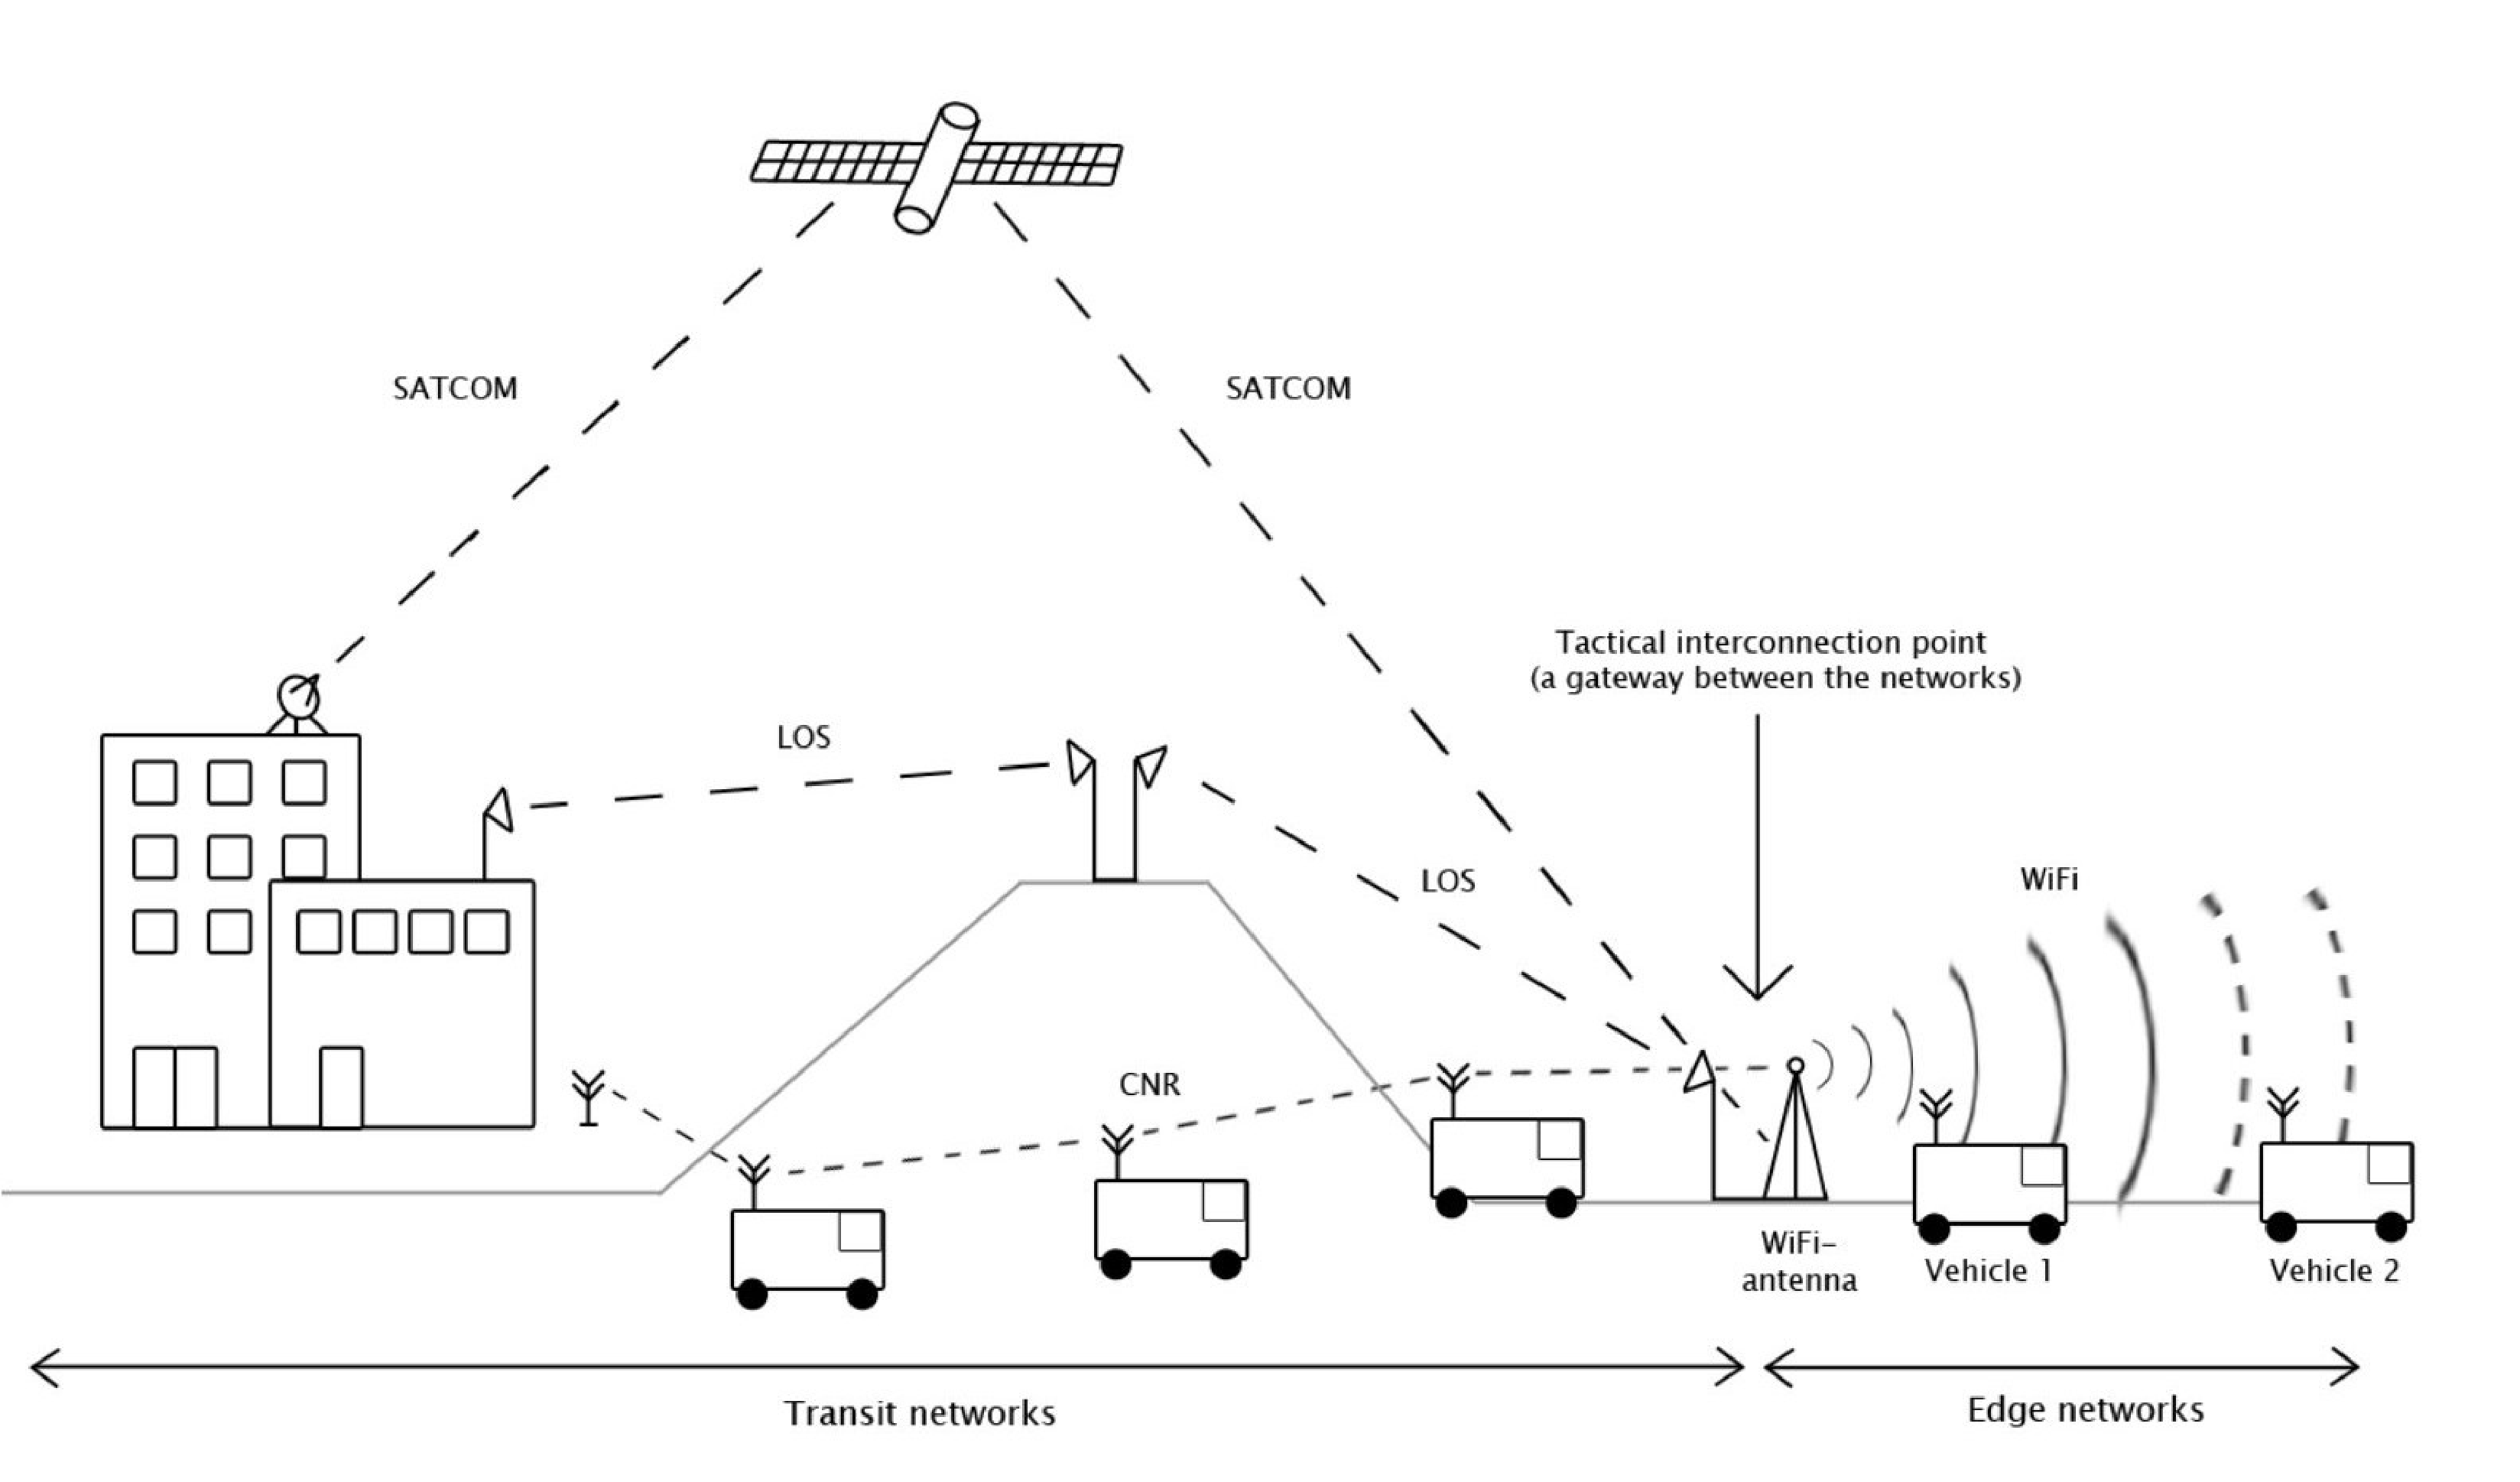
\includegraphics[scale=0.25]{images/networks_overview.pdf}
\caption{Overview of tested networks}
\label{figure-networks-overview}
\end{figure}

An infinite number of possible network combinations exists, so we have in this
thesis chosen to focus on five different network types identified by the task
group IST-118 for DIL-testing. We also investigated \gls{lte}, commonly known as
4G, a network technology which has become in widespread use in the latest years.
The reason for including LTE in addition to the ones from IST-118, is that the
Norwegian Defense is looking into the possibility of using LTE. Thus making it
interesting for us to investigate the performance under this type of network as
well. However, we eventually found out that LTE has gotten so fast and reliable,
that it is not really relevant from a DIL perspective. We therefor instead
looked into \gls{edge}, which is used as a fall back in geographical areas where
\gls{lte} and 3G is not available. The different networks and their properties
are summarized in \cref{table-network-types}.

\begin{table}[h]
\begin{tabular}{| l | l | l | l | l |}
\hline
  \textbf{Network} & \textbf{Data Rate} & \textbf{Delay} & \textbf{PER} \\ \hline
  Satellite Communication & 250 kbps & 550 ms & 0 \% \\ \hline
  Line of Sight & 2 mbps & 5 ms & 0 \% \\ \hline
  Wireless Fidelity (WiFi) 1 & 2 mbps & 100 ms & 1 \% \\ \hline
  WiFi 2 & 2 mbps & 100 ms & 20 \% \\ \hline
  Combat Net Radio with Forward Error Correction & 9.6 kbps & 100 ms & 1 \% \\ \hline
  Edge & 50/200 kbps & 200 ms & 0 \% \\ \hline
\end{tabular}
\caption{Different network types}
\label{table-network-types}
\end{table}


\section{Testing and Evaluation Tools}

In order to evaluate how our solution impacts the performance of Web services in
DIL environments, we needed some way of simulating such environments. Obviously,
we would have got the most realistic test environment by testing "out in the
field" ourself. However, this would require of a considerable amount of effort
and it would be difficult to reproduce the exact same environment and test
results. We therefor choose to instead emulate DIL networks. For testing we used
two approaches, the first one connecting two machines through a third machine.
The third machine used a component in the Linux kernel to control the flow
of the network traffic flowing through it, allowing us to simulate DIL networks.
The second approach involved using actual military equipment in a laboratory at
FFI. The benefit of using actual equipment, is that we got as realistic tests as
possible.


\subsection{\glsentrylong{netem}}

The Linux kernel offers a rich set of tools for managing and manipulating the
transmission of packets. \textbf{tc}(traffic control) is a Linux program to
configure and control the Linux kernels Network scheduler. \gls{netem} is an
enhancement of the traffic control facilities that allows us to control delay,
packet loss and other characteristics to packets outgoing from a selected
network interface\cite{man-netem}. These tools allow us to emulate many of the network
characteristics that makes DIL.

%Siter man-page om tc-netem
%Siter tldp -> Traffic Control HOWTO

\subsubsection{Delays}

NetEm can emulate delays on packets on a specific link. In
\cref{listing-netem-delay} we add a fixed delay on 100 ms to all packets going
out of local Ethernet.

\begin{lstlisting}[frame=single, caption="Emulating delay", label=listing-netem-delay]
  tc qdisc add dev eth0 root netem delay 100ms
\end{lstlisting}

\subsubsection{Corrupt rate}

The corrupt rate allows us to insert random data into a chosen percent of
packets.

\subsubsection{Data rate}

NetEm can set the data rate by delaying packets based on their packet size.

\subsection{Iperf 3}

iperf is a tool for performing network throughput measurements. Together with
ping we, used this tool to confirm that the \gls{netem} configuration worked as
expected.

\subsection{Wireshark}

Wireshark is a packet analyzer and allows for network analysis and let us see
the network traffic. Using this tool, we could investigate the behaviour of each
protocol used for testing.



\section{Test Setup}
\label{testing-environment}

The majority of testing was performed at the FFI-lab at Kjeller. All the test
applications consisted of one client and one Web service, where the client would
request the service for some sort of data. The client were hosted on one
computer and the service at an another computer. The majority of testing was
done using NetEm to emulate DIL networks, and some testing was done using actual
military radios. The machines used for testing is listed in
\cref{table-machines}.

\begin{table}[h]
\begin{tabular}{| l | l | l | l |}
\hline
  \textbf{Machine} & \textbf{Client} & \textbf{Application server} & \textbf{Router}\\ \hline
  Model & Asus UX 31A Notebook & HP EliteBook 6930p & HP Compaq Elite 8000 \\ \hline
  OS & Debian 8.2 & Ubuntu 14.04 & Ubuntu 14.04\\ \hline
  Kernel & 3.16.0-4-amd64 & 3.13.0-79-generic & 3.19.0-25-generic\\ \hline
  CPU & Intel i7 @ 1.90GHz & Intel Duo T95550 & Intel Quad Q9500 @ 2.83GHz \\ \hline
  Cores & 4 & 2 & 4\\ \hline
  Memory & 4 GB & 4 GB & 12 GB\\ \hline
  Network hardware & ASIX AX88772 USB 2.0 & 82567LM Gigabit & 82567LM-3 Gigabit\\ \hline
  Network interface capacity & 100 Mbit/s & 1 Gbit/s & 1 Gbit/s \\ \hline
\end{tabular}
\caption{Machines involved in the testing}
\label{table-machines}
\end{table}

\subsection{NetEm Setup}

In this setup, the client and Web service machines were connected to each other
through a third computer, acting as a router. This router machine had two
network cards and networked together the other machines by Ethernet cables. The
setup can been seen in \cref{figure-testing-environment}. In order for the
router machine to forward IP packets back and forth between the client and
server, IP forwarding was enabled on the kernel.

\begin{figure}[h]
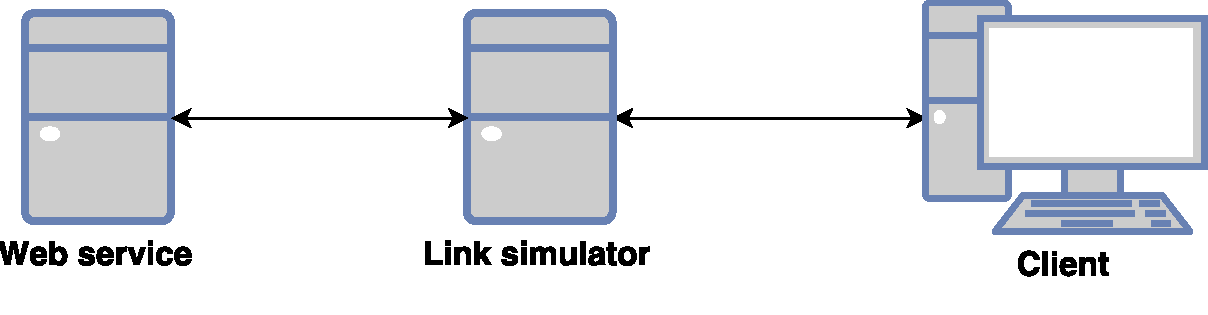
\includegraphics[scale=0.6]{images/testing_environment.pdf}
\caption{Testing environment}
\label{figure-testing-environment}
\end{figure}

The server and client are assigned an IP address in two different subnets.
This is done by the Linux network interface administration program
\textit{ifconfig}. In \cref{listing-ifconfig-client} the client machine is is
assigned the IP address 192.168.2.44.

\begin{lstlisting}[frame=single, caption="Configuring a network interface of the router", label=listing-ifconfig-client]
ifconfig eth0 192.168.2.1 up
\end{lstlisting}

After setting up the IP addresses we need to configure the routing so that the
kernel know where to route the network traffic. In this case we want all
traffic to go through the routing machine. In \cref{listing-routing} we
configure all IP traffic bound for the subnet 192.168.1.X to be routed through
the router machine with IP 192.168.2.1.

\begin{lstlisting}[frame=single, caption="Configuring routing rules for the client", label=listing-routing]
ip route add unicast 192.168.1.0/24 via 192.168.2.1
\end{lstlisting}

\subsubsection{Emulating different types of networks}

Since all network traffic passes through the routing machine, we can control
the flow of IP packets here. As previously discussed, we use NetEm.  For each
network configuration, a bash script is run. This script configures the
network interfaces in order to get the correct network behaviour. Both
interfaces are configured so the network is symmetrical in both directions.

\subsection{Military Radio Setup}

Although testing on regular machines with emulated network gives us a good
indication, to get as realistic results as possible we also performed tests on
military communication equipment. The setup is illustrated in
\cref{figure-radio-testing-environment}.

\begin{figure}[h]
\centering
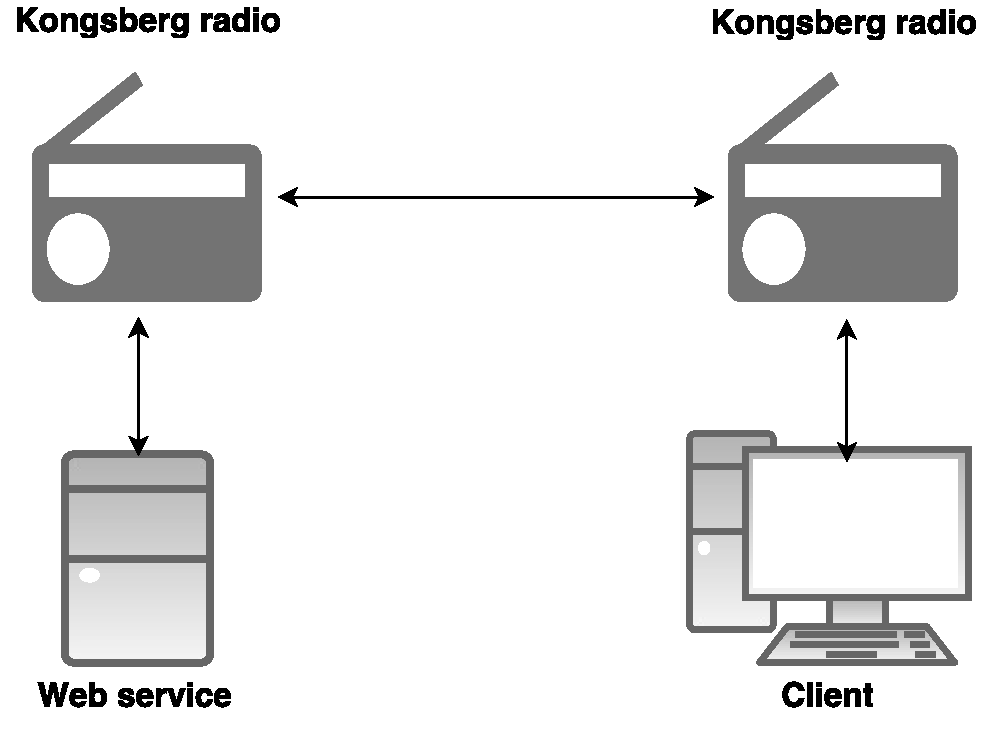
\includegraphics[scale=0.6]{images/radio_testing_environment.pdf}
\caption{Testing environment}
\label{figure-radio-testing-environment}
\end{figure}

\subsection{Proxy setup}

In order to enable the applications to tunnel all their HTTP traffic through our
proxy, we needed a way to setup a proxy without altering the applications
themselves. Fortunately, Java provide mechanisms to deal with
proxies\cite{oracle-proxy}. We configured the \gls{jvm} to get the applications
to tunnel all HTTP traffic through our proxy. This is done by setting properties
to the \gls{jvm}:


\begin{lstlisting}[frame=single, caption="Setting a proxy on the \gls{jvm}", label=test]
java -Dhttp.proxyHost=localhost \
-Dhttp.proxyPort=3001 \
-Dhttp.nonProxyHosts= \
-jar target/client.jar
\end{lstlisting}

In \cref{test} the application \textbf{client.jar} is started and all HTTP
traffic will go through the proxy server at localhost on port 3001.

\section{Test Execution}

For our tests we use originally used two different sets of applications. One for
W3C Web services and one for RESTful  Web services. While W3C web Services only
uses HTTP simply as a transport mechanism, REST utilizes the different HTTP
methods to indicate which operation to perform on a resource. Each test scenario
was therefor performed with both a W3C Web service application and RESTful Web
service application. Each service is deployed in Glassfish 4, while the client
is executed either from the command line or directly from the Netbeans IDEA.
Data being sent between the client and server is by default sent uncompressed.

During testing we discovered that especially CoAP was very sensitive to the
size of the messages being sent. We therefor developed a test application that
allowed the client to request a number of bytes from the server. This allowed us
to see how CoAP performed with different message sizes.

\subsection{NFFI W3C Web service}

For the purpose of testing W3C Web service applications we created a mock system
which allows a client to request a service to report positions of friendly
forces. The position reports use the \gls{nffi} format, which has an associated
XML schema with it. One test run is illustrated in \cref{figure-nffi-flow} and
consist of the client making a HTTP POST request to the Web service. Associated
with the request is an XML payload which tells the Web service which operation
to invoke. In our case, the service then returns an XML message containing a
large number of positions in the NFFI format.

\begin{figure}[h]
\centering
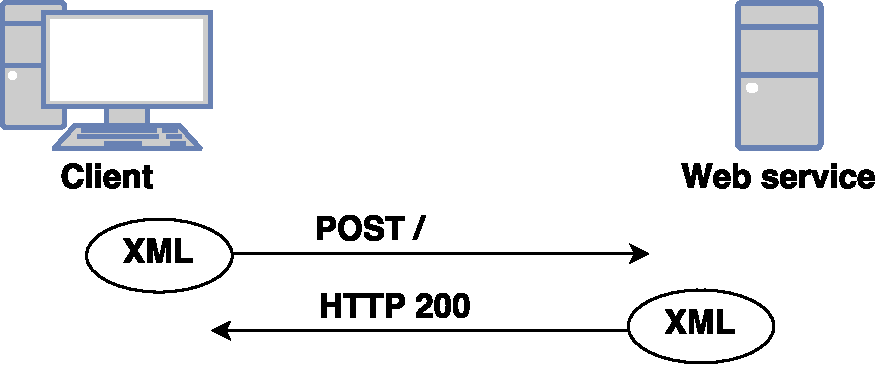
\includegraphics[scale=0.6]{images/nffi_flow.pdf}
\caption{NFFI Web service}
\label{figure-nffi-flow}
\end{figure}


\subsection{RESTful car Web service}

The RESTful Web service is an example service keeping order of cars in a ``car
system''. The service exposes an \gls{api} which offers different operations to
manage the car system. Clients can invoke these operations by using HTTP
requests and utilizing the associated HTTP method to indicate what to do with an
resource. Since RESTful services are payload agnostic, we choose JSON to
represent the data being sent between the server and the client. JSON is a
lightweight data-format. Each test run consist of a client sequentially invoking
the server with different API requests. The most common HTTP-methods GET, PUT,
POST, and DELETE are all part of the testing. An example, not inclusive, test run
is illustrated in \cref{figure-rest-flow}.

\begin{figure}[h]
\centering
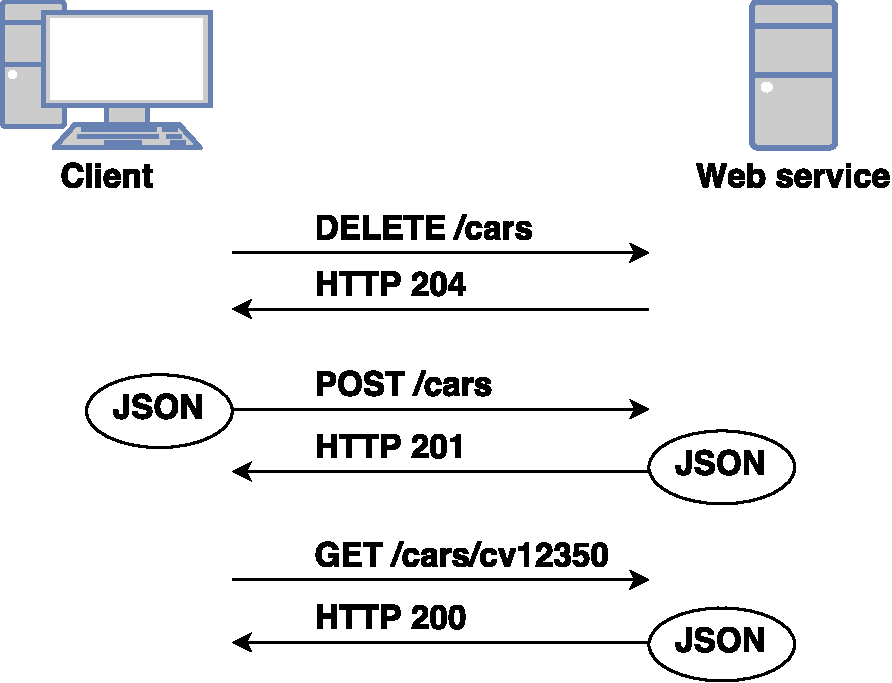
\includegraphics[scale=0.6]{images/rest_flow.pdf}
\caption{RESTful car service}
\label{figure-rest-flow}
\end{figure}


\subsection{Request size application}

This application allowed us to test with different message sizes.

\subsection{Test parameters}

The tests was performed with the following parameters.

\begin{itemize}
	\item GZIP compression on/off.
	\item Without and with proxies.
    \item Transport protocol used.
\end{itemize}


\section{Function tests}

The first phase of the testing was performed without any actual intended
limitations to the network. The objective of this testing is to validate that
the proxy is working correctly and have a benchmark to compare other results
with. This phase was again divided into two phases, one without the usage of
proxy and one with. Doing this allowed us to investigate any potential
overhead associated with the usage of the proxy. We used the NetEm setup with
a third machine acting as a router, although without any NetEm limitations
turned on.


\subsection{Results and Analysis}

Enabling compression yields an improvement in the performance, especially for
W3C Web services which had much larger messages. We also notice that HTTP and
CoAP has a almost identical performance, while AMQP has significant longer
average response time. Furthermore we can observe that the default solution
without proxies has the best performance in this unlimited network.

\begin{figure}[H]
\center
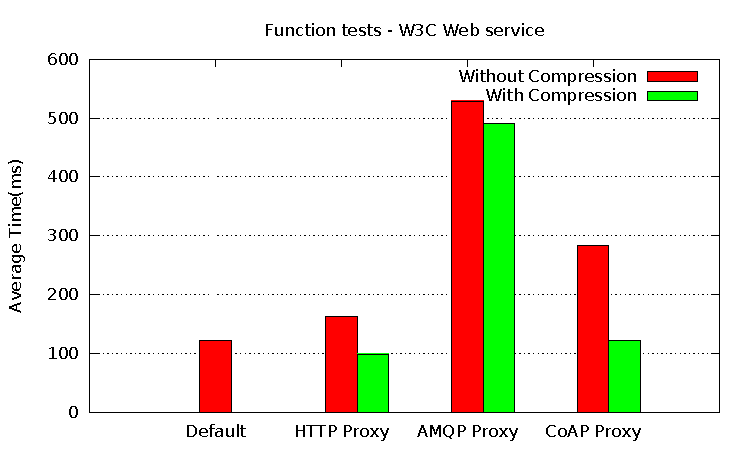
\includegraphics[scale=0.75]{../results/function_tests/nffi/out.pdf}
\caption{W3C Web services results}
\end{figure}

\begin{figure}[H]
\center
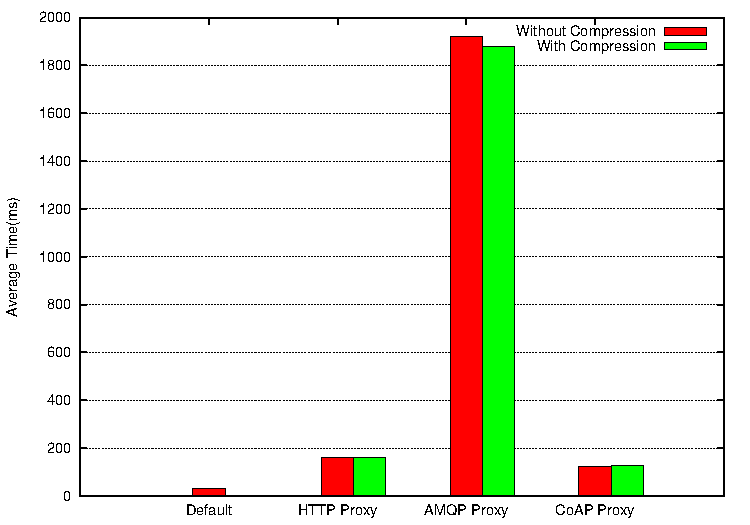
\includegraphics[scale=0.75]{../results/function_tests/rest/result.pdf}
\caption{REST results}
\end{figure}


\section{DIL Tests - Disconnected}

In this scenario we evaluate  the performance with the DIL characteristic
\textit{disconnected}, which refers to the network suddenly going down when the
application is sending data. The objective of this testing is to evaluate how
the proxy manages disconnects over longer periods of time. We define the success
criteria for this test to be that the client is able to eventually process his
request after the connection is reestablished. The client HTTP request should
not be interrupted in any way, other then it taking longer time to process the
request.

\subsection{Execution}

 The tests are performed on a unlimited network. During testing the Ethernet
 cable between the client machine and the router was removed for about 60
 seconds. It was then reconnected.

\subsection{Results and Analysis}

For both the REST and W3C Web service test scenarios the results were identical.
Without using proxies, the connection timed out and the applications were unable
to continue. With proxies the connection did not time out, and the protocols
retransmission mechanism were able to continue transmission when connection was
reestablished.

\begin{table}[h!]
\begin{tabular}{| l | l |}
\hline
  \textbf{Test} & \textbf{Result} \\ \hline
  Without proxy & Connection timeout \\ \hline
  Proxy with HTTP & Success \\ \hline
  Proxy with AMQP & Success \\ \hline
  Proxy with CoAP & Success \\ \hline
\end{tabular}
\caption{W3C Web service results}
\end{table}

\begin{table}[h!]
\begin{tabular}{| l | l |}
\hline
  \textbf{Test} & \textbf{Result} \\ \hline
  Without proxy & Connection timeout \\ \hline
  Proxy with HTTP & Success \\ \hline
  Proxy with AMQP & Success \\ \hline
  Proxy with CoAP & Success \\ \hline
\end{tabular}
\caption{RESTful Web service results}
\end{table}



\section{DIL Tests - Intermittent}

\textit{Intermittent} refers to the network connection being lost, but then
regained again. The objective of this testing is to evaluate how the proxy
manages frequent temporary loss of connections. The success criteria is the same
as for disconnected, the client should not notice any disruption of service.

\subsection{Execution}

Not done yet. Similar to disconnect.

\subsection{Results}

\begin{table}[H]
\begin{tabular}{| l | l |}
\hline
  \textbf{Test} & \textbf{Result} \\ \hline
  Without proxy & X \\ \hline
  Proxy with HTTP & X \\ \hline
  Proxy with AMQP & X \\ \hline
  Proxy with CoAP & X \\ \hline
\end{tabular}
\caption{W3C Web service results}
\end{table}

\begin{table}[H]
\begin{tabular}{| l | l |}
\hline
  \textbf{Test} & \textbf{Result} \\ \hline
  Without proxy & X \\ \hline
  Proxy with HTTP & X \\ \hline
  Proxy with AMQP & X \\ \hline
  Proxy with CoAP & X \\ \hline
\end{tabular}
\caption{RESTful Web service results}
\end{table}

\section{DIL Tests - Limited}

The third DIL characteristic, \textit{limited}, refers to different ways a
network can be limited. This includes high delays, packet loss and low
bandwidth. In this section we present the testing performed for the different
types of networks identified in \cref{table-network-types}.



\subsection{Satellite communication}

In this test scenario we emulate \gls{satcom}. With satellite communication
all data is relayed through an communication satellite in orbit around
the earth. This type of communication is characterized by its low data rate
and high delay.

\subsubsection{Results and analysis}

AMQP has a very long response time for both test scenarios, while also CoAP
struggles with large uncompressed XML messages of the NFFI service. For both
with and without compression, we observe that employing HTTP proxies yields a
small improvement of performance, compared to the default. We can also notice
that for the RESTful service, CoAP has better performance than default, and
similar performance to HTTP proxies.

\begin{figure}[H]
\center
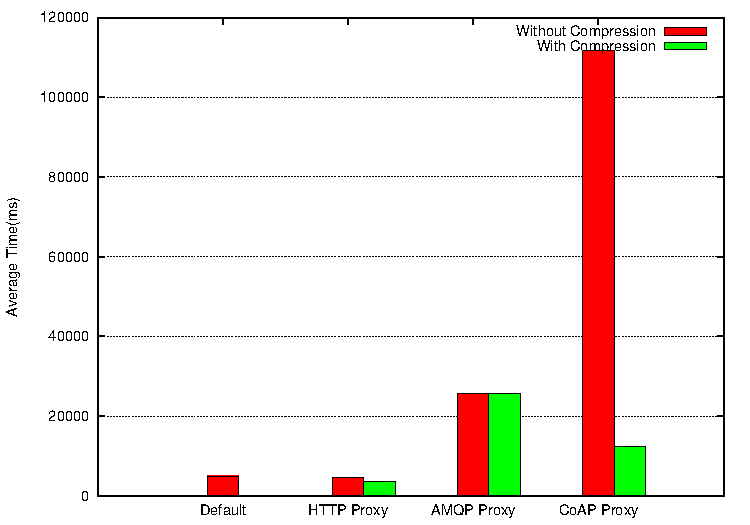
\includegraphics[scale=0.75]{../results/satellite/nffi/result.pdf}
\caption{W3C Web services results}
\end{figure}

\begin{figure}[H]
\center
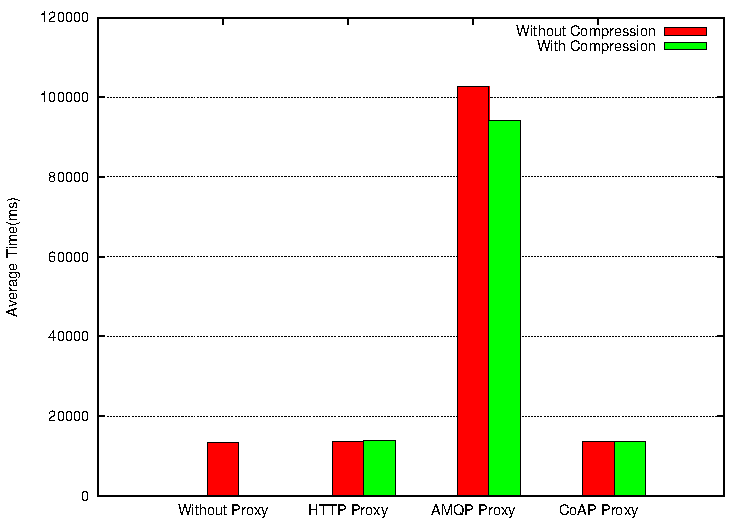
\includegraphics[scale=0.75]{../results/satellite/rest/result.pdf}
\caption{REST results}
\end{figure}

\subsection{Line-of-Sight}

In this test scenario we emulate so-called \gls{los} networks, which are
characterized by being a radio-based type of network with no physical obstacles
between the nodes in the network. High data rate, low delay and zero error.

\subsubsection{Results and analysis}

Again we notice CoAP really struggling with uncompressed XML messages, as well
as AMQP performing significantly poorer than the other protocols. However,
when the message is compressed CoAP has roughly equal performance as the
default. When we look on the RESTful test application results, we see that
CoAP performs better than default and HTTP with compressed messages.

\begin{figure}[H]
\center
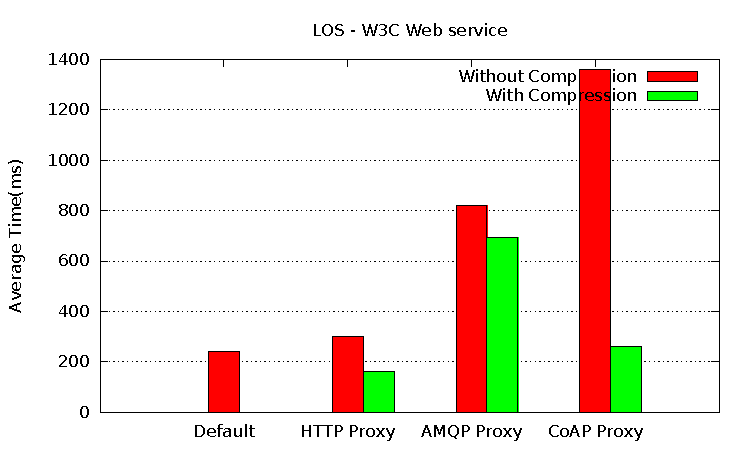
\includegraphics[scale=0.75]{../results/los/nffi/out.pdf}
\caption{W3C Web services results}
\end{figure}

\begin{figure}[H]
\center
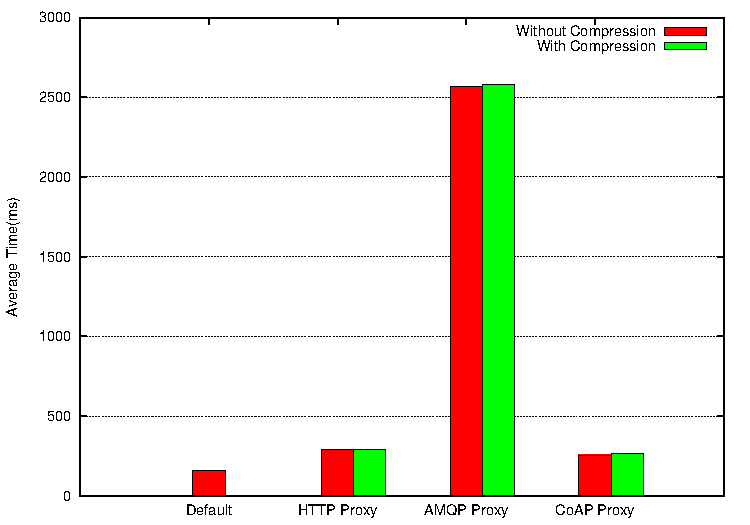
\includegraphics[scale=0.75]{../results/los/rest/result.pdf}
\caption{REST results}
\end{figure}



\subsection{WiFi 1}

With this type of network we emulate communication over WiFi where the
conditions are relatively good. The data rate is high, the delay is moderate
and the packet error rate is around 1 \%.

\subsubsection{Results and analysis}

HTTP proxies with compression enabled yields the best performance. CoAP has
worse performance than the HTTP proxies, but roughly equal for the compressed
REST tests.


\begin{figure}[H]
\center
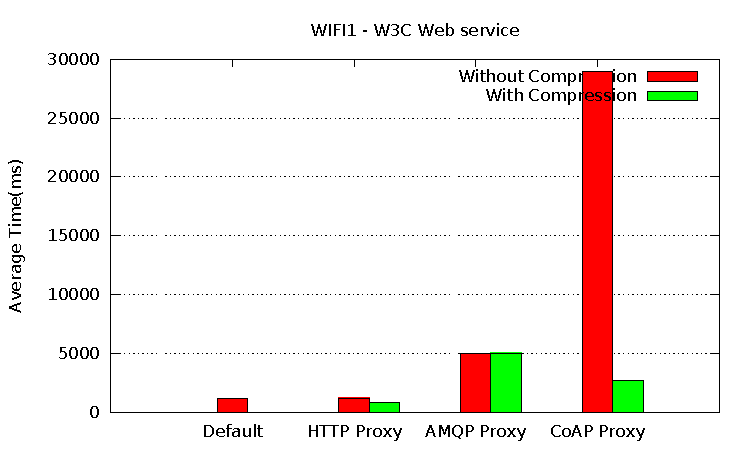
\includegraphics[scale=0.75]{../results/wifi1/nffi/out.pdf}
\caption{W3C Web services results}
\end{figure}

\begin{figure}[H]
\center
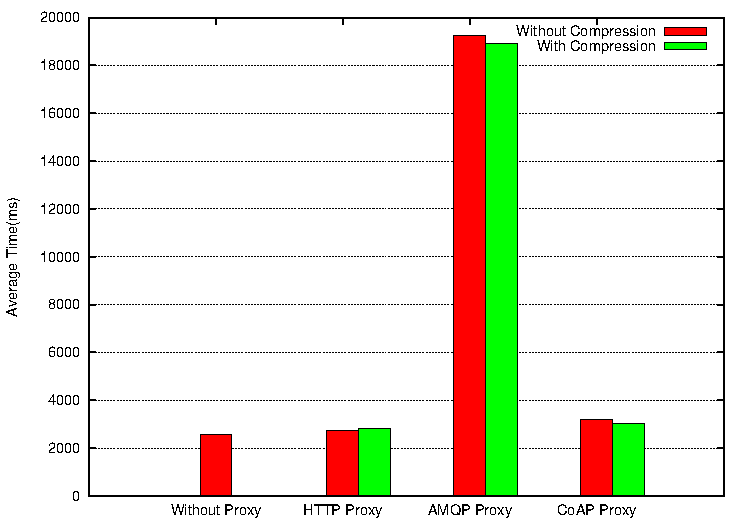
\includegraphics[scale=0.75]{../results/wifi1/rest/result.pdf}
\caption{REST results}
\end{figure}


\subsection{WiFi 2}

This type of network also emulate wireless communication, but instead in the
``outer'' areas of the wireless range. It has good data rate, moderate delay
and very high packet error rate(20 \%).


\subsubsection{Results and analysis}

Compared to WiFi 1, we see that all response times has increased
significantly. The importance of compression has increased, the tests with
compression turned on yields a large performance increase. In the uncompressed
NFFI test scenario, CoAP reached it's time out, and were unable to finish. In
the scenarios where CoAP did finish it still performed worse than default and
HTTP. HTTP proxies with compression yielded the best results.

\begin{figure}[H]
\center
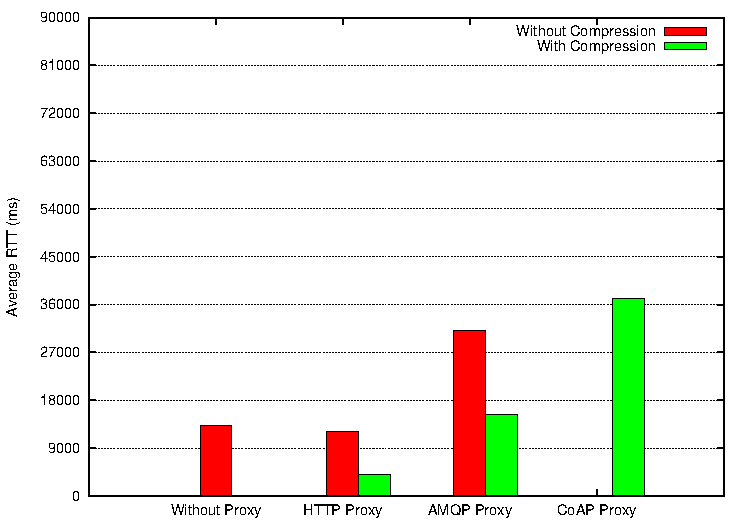
\includegraphics[scale=0.75]{../results/wifi2/nffi/result.pdf}
\caption{W3C Web services results}
\end{figure}

\begin{figure}[H]
\center
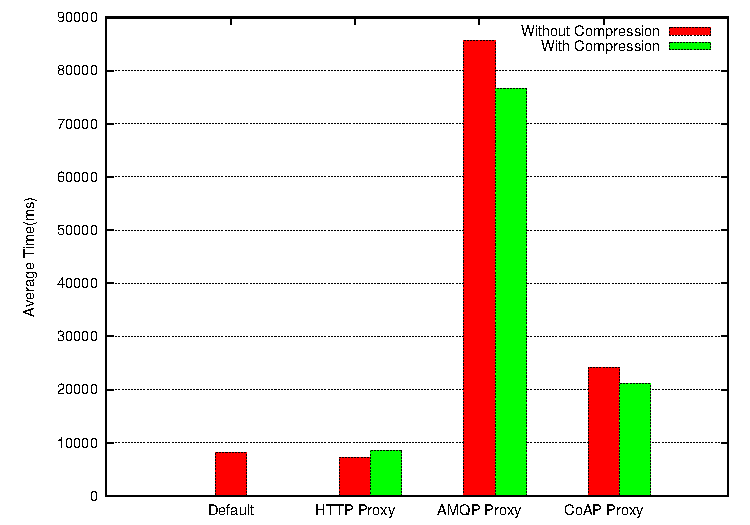
\includegraphics[scale=0.75]{../results/wifi2/rest/result.pdf}
\caption{REST results}
\end{figure}

\subsection{Combat Net Radio with Forward Error Correction}

This type of network is characterized by very low data rate, moderate timeout
and packet error rate on around 1 \%.


\subsubsection{Results and analysis}

Again we can observe the importance of compression in this type of networks.
CoAP has the best performance.

\begin{figure}[H]
\center
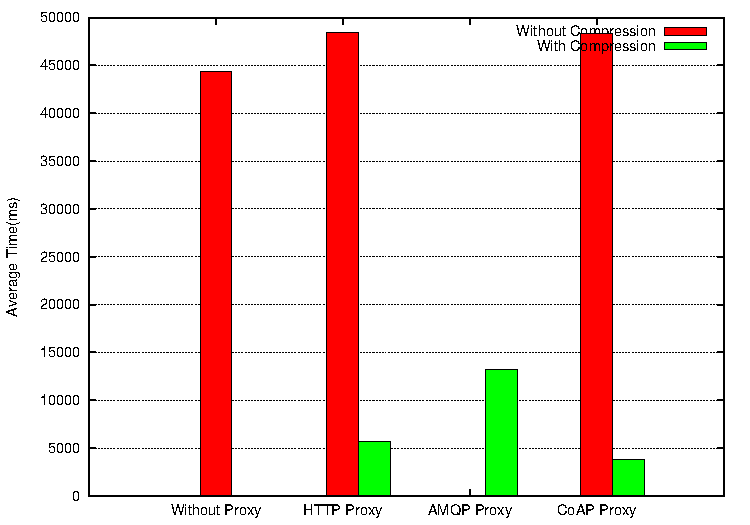
\includegraphics[scale=0.75]{../results/cnr/nffi/result.pdf}
\caption{W3C Web services results}
\end{figure}

\begin{figure}[H]
\center
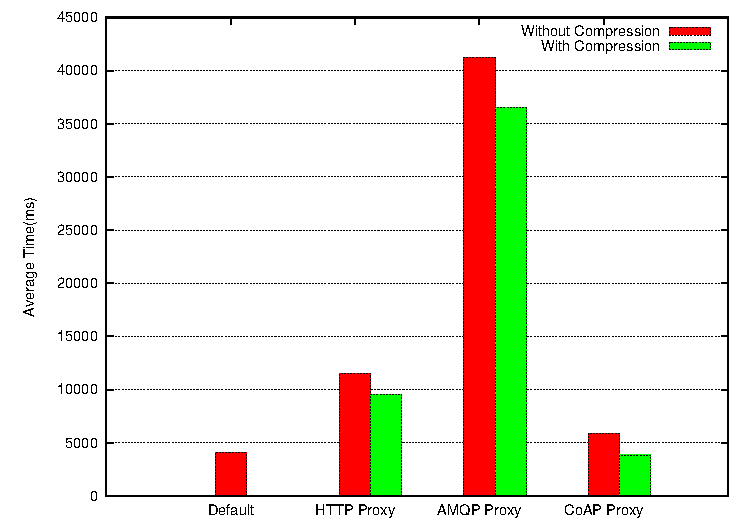
\includegraphics[scale=0.75]{../results/cnr/rest/result.pdf}
\caption{REST results}
\end{figure}


\subsection{EDGE}

About this type of network.

\subsubsection{Results and analysis}

\begin{figure}[H]
\center
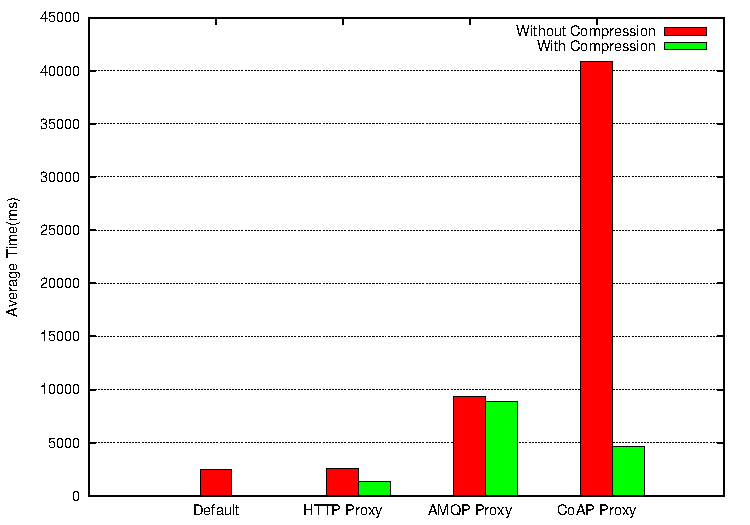
\includegraphics[scale=0.75]{../results/edge/nffi/result.pdf}
\caption{W3C Web services results}
\end{figure}

\begin{figure}[H]
\center
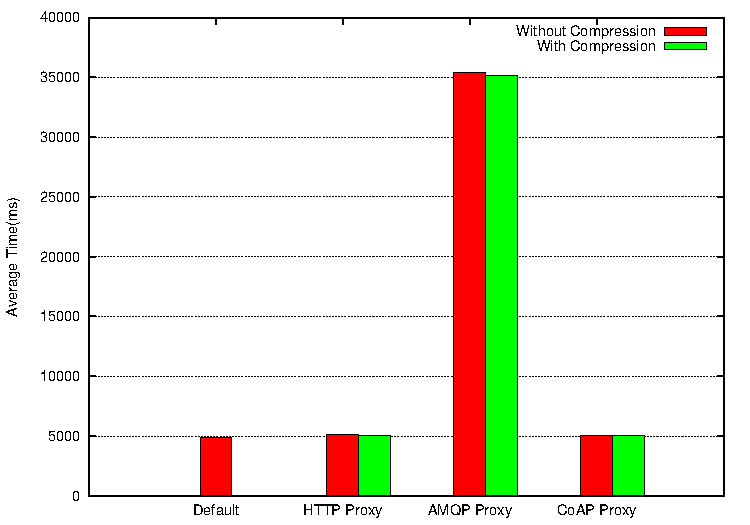
\includegraphics[scale=0.75]{../results/edge/rest/result.pdf}
\caption{REST results}
\end{figure}

\subsection{Kongsberg Radio}

Two KDA WM 600.


\subsubsection{Results and analysis}

For NFFI tests, compression yields a lot of increase in performance.

\begin{figure}[H]
\center
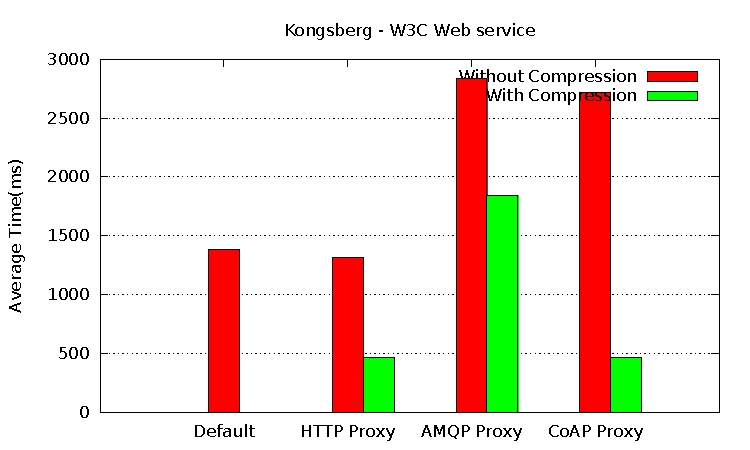
\includegraphics[scale=0.75]{../results/kongsberg/nffi/out.pdf}
\caption{W3C Web services results}
\end{figure}

\begin{figure}[H]
\center
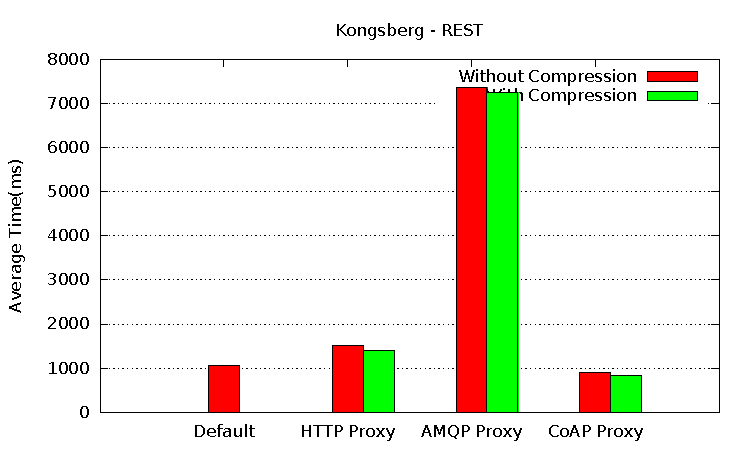
\includegraphics[scale=0.75]{../results/kongsberg/rest/out.pdf}
\caption{REST results}
\end{figure}



\section{Summary}

In this section the results from the tests are presented. These results lead up
to the discussion and conclusion in the next chapter.

\begin{itemize}
\item AMQP has the worst performance in almost every test scenario.
\item Compression almost always yields in performance increase.
\item CoAP struggles with larger messages.
\item CoAP has the best performance with smaller messages in networks with low data rate.
\end{itemize}


\chapter{Conclusion and Future Work}
\label{chapter:conclusion}

\section{Conclusion}
Revisit problem statement.

\section{Future Work}

IPSEC.

\pagebreak
\printbibliography{}
\printglossaries{}

\begin{appendices}

\chapter{Network emulating}

\label{appendix-netem-scripts}

This appendix lists the different scripts that was used to emulate the different
types of networks.

\section{\gls{satcom}}

\begin{lstlisting}[frame=single, caption="Emulating SATCOM", label=satcom]
  tc qdisc add dev eth0 parent 1:1 handle 10: \
    netem delay XX ms
\end{lstlisting}

\section{\gls{los}}
Placeholder

\section{WiFi 1}
Placeholder

\section{WiFi 2}
Placeholder

\section{\gls{cnr}}
Placeholder

\section{\gls{edge}}
Placeholder



\chapter{Results}
\label{appendix-results}

In this appendix the data material from the evaluations is presented. Each test
case was run a number of times, ranging from 10 to 100 runs. Then the mean,
\gls{std} and variance was calculated by using the Apache Commons
Mathematics Library\cite{apache-math-homepage}. An example of how this was done
running NFFI Web service tests can be seen in \cref{listing:statistics}.

\lstinputlisting[frame=single, language=java, firstnumber=1, caption="Calculating statistic values", label=listing:statistics]{listings/stats.java}


We also performed an analysis of the network utilization using Wireshark. This was done by starting a packet capture, running one test run and inspecting the packet capture. The calculation of bytes sent and received was done by:

\begin{enumerate}
    \item Starting Wireshark on the same machine as the client.
    \item Filtering traffic to only show traffic between the IP addresses of the client and Web service.
    \item Using the TCP/UDP conversation view of Wireshark.
\end{enumerate}

\section{Function Tests}

\begin{itemize}
	\item Ping measured to \textasciitilde 1 ms.
	\item Iperf3 measured data rate: 7.76 Mbits/sec.
\end{itemize}


\subsection{NFFI Web Service}

\begin{table}[H]
\begin{tabular}{llllr}
\hline
 Test                   &   Mean &   \gls{std} &   Variance &   Test runs \\
\hline
  Without proxy & 122 ms & 29 & 869 & 300 \\
  Proxy with HTTP & 163 ms & 25 & 601 & 300 \\
  Proxy with HTTP \& GZIP & 99 ms & 19 & 346 & 300 \\
  Proxy with AMQP & 529 ms & 60 & 3690 & 300 \\
  Proxy with AMQP \& GZIP & 490 ms & 62 & 3847 & 300\\
  Proxy with CoAP & 285 ms & 33 & 1122 & 300 \\
  Proxy with CoAP \& GZIP & 122 ms & 33 & 1091 & 300 \\
\end{tabular}
\caption{Mean response times of NFFI Web Service - Function Test}
\end{table}

\begin{table}[H]
\begin{tabular}{lrrrr}
\hline
\multicolumn{1}{l}{}                  & \multicolumn{2}{c}{Client -> Web service}                           & \multicolumn{2}{c}{Web service -> Client}                           \\
\multicolumn{1}{l}{Test} & \multicolumn{1}{l}{Packets sent} & \multicolumn{1}{l}{Bytes sent} & \multicolumn{1}{l}{Packets sent} & \multicolumn{1}{l}{Bytes sent} \\ \hline
Without Proxy                   & 51             & 4609           & 46             & 51706          \\
Proxy with HTTP                 & 45             & 5392           & 44             & 55489          \\
Proxy with HTTP \& GZIP         & 13             & 2781           & 13             & 2585           \\
Proxy with AMQP                 & 73             & 10284          & 94             & 64472          \\
Proxy with AMQP \& GZIP         & 76             & 11309          & 77             & 66562          \\
Proxy with CoAP                 & 101            & 8120           & 101            & 57137          \\
Proxy with CoAP \& GZIP         & 11             & 1680           & 11             & 5502           \\
\end{tabular}
\caption{Wireshark analysis of NFFI Web Service - Function Test}
\end{table}

\subsection{RESTful Car System}

\begin{table}[H]
\begin{tabular}{lrrrr}
\hline
 Test                   &   Mean &   Std. Deviation &   Variance &   Test runs \\
\hline
 Without proxy          &     30 &               12 &        147 &         100 \\
 Proxy with HTTP        &    160 &               97 &       9486 &         100 \\
 Proxy with HTTP \& GZIP &    159 &               76 &       5822 &         100 \\
 Proxy with AMQP        &   1919 &              128 &      16388 &         100 \\
 Proxy with AMQP \& GZIP &   1880 &              109 &      11919 &         100 \\
 Proxy with CoAP        &    124 &               64 &       4079 &         100 \\
 Proxy with CoAP \& GZIP &    128 &               64 &       4109 &         100 \\
\hline
\end{tabular}
\caption{Mean response times of RESTful Car System - Function Test}
\end{table}

\begin{table}[H]
\begin{tabular}{lrrrr}
\hline
\multicolumn{1}{l}{}                  & \multicolumn{2}{c}{Client -> Web service}                           & \multicolumn{2}{c}{Web service -> Client}                           \\
\multicolumn{1}{l}{Test} & \multicolumn{1}{l}{Packets sent} & \multicolumn{1}{l}{Bytes sent} & \multicolumn{1}{l}{Packets sent} & \multicolumn{1}{l}{Bytes sent} \\ \hline
Without Proxy                   & 25             & 4738           & 21             & 5638           \\
Proxy with HTTP                 & 28             & 9677           & 26             & 15147          \\
Proxy with HTTP \& GZIP         & 28             & 8735           & 28             & 12993          \\
Proxy with AMQP                 & 180            & 30366          & 203            & 47484          \\
Proxy with AMQP \& GZIP         & 190            & 30224          & 207            & 42314          \\
Proxy with CoAP                 & 12             & 4757           & 12             & 8369           \\
Proxy with CoAP \& GZIP         & 12             & 3943           & 12             & 6053           \\
\end{tabular}

\caption{Wireshark analysis of RESTful Car System - Function Test}
\end{table}


\subsection{Request Message}

\begin{table}[H]
\begin{tabular}{lrrr}
\hline
 Protocol   &   1 byte &   2500 bytes &   100 000 bytes \\
\hline
 Default    &       43 &            8 &             112 \\
 HTTP       &       53 &           54 &             121 \\
\hline
\end{tabular}
\caption{Mean response times of Request Message - Function Test}
\end{table}


\section{Satellite Tests}

\begin{itemize}
	\item Ping measured to \textasciitilde 1100 ms.
	\item Iperf3 measured data rate: 402/291 Kbits/sec.
\end{itemize}

\subsection{NFFI Web Service}

\begin{table}[H]
\begin{tabular}{llrrr}
\hline
 Test                   & Mean      &   Std. Deviation &   Variance &   Test runs \\
\hline
 Without proxy          & 4978 ms   &              378 &     142762 &          10 \\
 Proxy with HTTP        & 4511 ms   &               71 &       5009 &          10 \\
 Proxy with HTTP \& GZIP & 3530 ms   &               50 &       2472 &          10 \\
 Proxy with AMQP        & 25709 ms  &              793 &     628112 &          10 \\
 Proxy with AMQP \& GZIP & 25780 ms  &             1159 &    1343947 &          10 \\
 Proxy with CoAP        & 111636 ms &               59 &       3437 &          10 \\
 Proxy with CoAP \& GZIP & 12347 ms  &               41 &       1652 &          10 \\
\hline
\end{tabular}
\caption{Mean response times of NFFI Web Service - Satellite test}
\end{table}

\begin{table}[H]
\begin{tabularx}{\textwidth}{lXXXX}
\hline
\multicolumn{1}{l}{}                  & \multicolumn{2}{c}{Client->Web service}                           & \multicolumn{2}{c}{Web service->Client}                           \\
\multicolumn{1}{l}{Test} & \multicolumn{1}{l}{P. sent} & \multicolumn{1}{l}{B. sent} & \multicolumn{1}{l}{P.sent} & \multicolumn{1}{l}{B.sent} \\ \hline
Without Proxy                   & 54             & 4811           & 47             & 51623          \\
Proxy with HTTP                 & 47             & 5532           & 45             & 55563          \\
Proxy with HTTP \& GZIP         & 16             & 2987           & 14             & 7177           \\
Proxy with AMQP                 & 88             & 11342          & 102            & 65040          \\
Proxy with AMQP \& GZIP         & 71             & 9731           & 68             & 15679          \\
Proxy with CoAP                 & 101            & 7810           & 101            & 56827          \\
Proxy with CoAP \& GZIP         & 11             & 1668           & 11             & 5486           \\
\end{tabularx}

\caption{Wireshark analysis of NFFI Web Service - Satellite test}
\end{table}

\subsection{RESTful Car System}

\begin{table}[H]
\begin{tabular}{llrrr}
\hline
 Test                   & Mean      &   Std. Deviation &   Variance &   Test runs \\
\hline
 Without proxy          & 13386 ms  &              401 &     160523 &          10 \\
 Proxy with HTTP        & 13643 ms  &              427 &     182464 &          10 \\
 Proxy with HTTP \& GZIP & 13825 ms  &              897 &     804893 &          10 \\
 Proxy with AMQP        & 102748 ms &             3065 &    9396423 &          10 \\
 Proxy with AMQP \& GZIP & 94163 ms  &              568 &     322659 &          10 \\
 Proxy with CoAP        & 13545 ms  &              217 &      47260 &          10 \\
 Proxy with CoAP \& GZIP & 13562 ms  &              223 &      49522 &          10 \\
\hline
\end{tabular}
\caption{Mean response times of RESTful Car System - Satellite test}
\end{table}

\begin{table}[H]
\begin{tabularx}{\textwidth}{lXXXX}
\hline
\multicolumn{1}{l}{}                  & \multicolumn{2}{c}{Client->Web service}                           & \multicolumn{2}{c}{Web service->Client}                           \\
\multicolumn{1}{l}{Test} & \multicolumn{1}{l}{P. sent} & \multicolumn{1}{l}{B. sent} & \multicolumn{1}{l}{P.sent} & \multicolumn{1}{l}{B.sent} \\ \hline
Without Proxy                   & 27             & 4878           & 22             & 5712           \\
Proxy with HTTP                 & 26             & 9538           & 25             & 15075          \\
Proxy with HTTP \& GZIP         & 30             & 8873           & 28             & 13010          \\
Proxy with AMQP                 & 244            & 34841          & 238            & 49914          \\
Proxy with AMQP \& GZIP         & 240            & 33739          & 240            & 44625          \\
Proxy with CoAP                 & 12             & 4751           & 12             & 8380           \\
Proxy with CoAP \& GZIP         & 12             & 3940           & 12             & 6063           \\
\end{tabularx}

\caption{Wireshark analysis of RESTful Car System - Satellite test}
\end{table}

\subsection{Request Message}

\begin{table}[H]
\begin{tabularx}{\textwidth}{llll}
\hline
 Protocol   & 1 byte   & 2500 bytes   & 100 000 bytes   \\
\hline
 Default    & 2246 ms  & 2210 ms      & 3987 ms         \\
 HTTP       & 1121 ms  & 1121 ms      & 4035 ms         \\
 AMQP       & 7939 ms  & 8210 ms      & 9388 ms         \\
\hline
\end{tabularx}
\caption{Request message results}
\end{table}


\section{Line-of-Sight Tests}

\begin{itemize}
	\item Ping measured to \textasciitilde 11 ms.
	\item Iperf3 measured data rate: 2.34/2.15 Mbits/sec.
\end{itemize}

\subsection{NFFI Web Service}

\begin{table}[H]
\begin{tabular}{llllr}
\hline
 Test                   &   Mean &   STD &   Variance &   Test runs \\
\hline
  Without proxy & 242 ms & 26 & 663 & 100 \\
  Proxy with HTTP & 299 ms & 40 & 1577 & 100 \\
  Proxy with HTTP \& GZIP & 162 ms & 34 & 1177 & 100 \\
  Proxy with AMQP & 821 ms & 60 & 3588 & 100 \\
  Proxy with AMQP \& GZIP & 693 ms & 75 & 5632 & 100\\
  Proxy with CoAP & 1359 ms & 45 & 1988 & 100 \\
  Proxy with CoAP \& GZIP & 262 ms & 36 & 1314 & 100 \\
\end{tabular}
\caption{Mean response times of NFFI Web Service - LOS test}
\end{table}

\begin{table}[H]
\begin{tabularx}{\textwidth}{lXXXX}
\hline
\multicolumn{1}{l}{}                  & \multicolumn{2}{c}{Client->Web service}                           & \multicolumn{2}{c}{Web service->Client}                           \\
\multicolumn{1}{l}{Test} & \multicolumn{1}{l}{P. sent} & \multicolumn{1}{l}{B. sent} & \multicolumn{1}{l}{P.sent} & \multicolumn{1}{l}{B.sent} \\ \hline
Without Proxy                   & 46             & 4267           & 43             & 51343          \\
Proxy with HTTP                 & 43             & 5260           & 44             & 55489          \\
Proxy with HTTP \& GZIP         & 14             & 2847           & 13             & 7103           \\
Proxy with AMQP                 & 68             & 9950           & 91             & 64274          \\
Proxy with AMQP \& GZIP         & 54             & 8529           & 59             & 15044          \\
Proxy with CoAP                 & 101            & 7565           & 101            & 56582          \\
Proxy with CoAP \& GZIP         & 11             & 1647           & 11             & 5466           \\
\end{tabularx}

\caption{Wireshark analysis of NFFI Web Service - LOS test}
\end{table}


\subsection{RESTful Car System}

\begin{table}[H]
\begin{tabularx}{\textwidth}{llrrr}
\hline
 Test                   & Mean    &   Std. Deviation &   Variance &   Test runs \\
\hline
 Without proxy          & 156 ms  &               15 &        214 &         100 \\
 Proxy with HTTP        & 288 ms  &               77 &       6000 &         100 \\
 Proxy with HTTP \& GZIP & 292 ms  &               86 &       7382 &         100 \\
 Proxy with AMQP        & 2567 ms &              102 &      10333 &         100 \\
 Proxy with AMQP \& GZIP & 2579 ms &              129 &      16595 &         100 \\
 Proxy with CoAP        & 256 ms  &               69 &       4775 &         100 \\
 Proxy with CoAP \& GZIP & 263 ms  &               69 &       4693 &         100 \\
\hline
\end{tabularx}
\caption{Mean response times of RESTful Car System - LOS test}
\end{table}

\begin{table}[H]
\begin{tabularx}{\textwidth}{lXXXX}
\hline
\multicolumn{1}{l}{}                  & \multicolumn{2}{c}{Client->Web service}                           & \multicolumn{2}{c}{Web service->Client}                           \\
\multicolumn{1}{l}{Test} & \multicolumn{1}{l}{P. sent} & \multicolumn{1}{l}{B. sent} & \multicolumn{1}{l}{P.sent} & \multicolumn{1}{l}{B.sent} \\ \hline
Without Proxy                   & 25             & 4738           & 21             & 5638           \\
Proxy with HTTP                 & 28             & 9704           & 26             & 15201          \\
Proxy with HTTP \& GZIP         & 24             & 8486           & 24             & 8486           \\
Proxy with AMQP                 & 189            & 30968          & 201            & 47352          \\
Proxy with AMQP \& GZIP         & 187            & 29979          & 201            & 41927          \\
Proxy with CoAP                 & 12             & 4756           & 12             & 8397           \\
Proxy with CoAP \& GZIP         & 12             & 3934           & 12             & 6059           \\
\end{tabularx}

\caption{Wireshark analysis of RESTful Car System - LOS test}
\end{table}

\subsection{Request Message}
\begin{table}[H]
\begin{tabularx}{\textwidth}{llll}
\hline
 Protocol   & 1 byte   & 2500 bytes   & 100 000 bytes   \\
\hline
 Default    & 64 ms    & 27 ms        & 420 ms          \\
 HTTP       & 62 ms    & 68 ms        & 423 ms          \\
 AMQP       & 214 ms   & 274 ms       & 592 ms          \\
\hline
\end{tabularx}
\caption{Mean response times of Request Message - LOS Test}
\end{table}


\section{WiFi 1 tests}

\begin{itemize}
	\item Ping measured to \textasciitilde 200 ms.
	\item Iperf3 measured data rate: 1.72/1.67 Mbits/sec.
\end{itemize}


\subsection{NFFI Web Service}

\begin{table}[H]
\begin{tabular}{llllr}
\hline
 Test                   &   Mean &   STD &   Variance &   Test runs \\
\hline
  Without proxy & 1202 ms & 162 & 26326 & 100 \\
  Proxy with HTTP & 1213 ms & 354 & 125628 & 100 \\
  Proxy with HTTP \& GZIP & 820 ms & 154 & 23586 & 100 \\
  Proxy with AMQP & 5026 ms & 460 & 211385 & 100 \\
  Proxy with AMQP \& GZIP & 4964 ms & 637 & 405390 & 100\\
  Proxy with CoAP & 25615 ms & 3185 & 10142866 & 10 \\
  Proxy with CoAP \& GZIP & 2823 ms & 1425 & 2031770 & 100 \\
\end{tabular}
\caption{Mean response times of NFFI Web Service - WiFi 1 test}
\end{table}

\begin{table}[H]
\begin{tabularx}{\textwidth}{lXXXX}
\hline
\multicolumn{1}{l}{}                  & \multicolumn{2}{c}{Client->Web service}                           & \multicolumn{2}{c}{Web service->Client}                           \\
\multicolumn{1}{l}{Test} & \multicolumn{1}{l}{P. sent} & \multicolumn{1}{l}{B. sent} & \multicolumn{1}{l}{P.sent} & \multicolumn{1}{l}{B.sent} \\ \hline
Without Proxy                   & 50             & 4531           & 45             & 51475          \\
Proxy with HTTP                 & 45             & 5560           & 45             & 57003          \\
Proxy with HTTP \& GZIP         & 13             & 2793           & 14             & 8297           \\
Proxy with AMQP                 & 76             & 10494          & 93             & 64406          \\
Proxy with AMQP \& GZIP         & 60             & 8941           & 60             & 15126          \\
Proxy with CoAP                 & 104            & 9214           & 104            & 58817          \\
Proxy with CoAP \& GZIP         & 11             & 1682           & 11             & 5491           \\
\end{tabularx}

\caption{Wireshark analysis of NFFI Web Service - WiFi 1 test}
\end{table}

\subsection{RESTful Car System}

\begin{table}[H]
\begin{tabularx}{\textwidth}{llrrr}
\hline
 Test                   & Mean     &   Std. Deviation &   Variance &   Test runs \\
\hline
 Without proxy          & 2581 ms  &              265 &      70406 &         100 \\
 Proxy with HTTP        & 2728 ms  &              270 &      73000 &         100 \\
 Proxy with HTTP \& GZIP & 2818 ms  &              369 &     136307 &         100 \\
 Proxy with AMQP        & 19236 ms &              490 &     240174 &          10 \\
 Proxy with AMQP \& GZIP & 18925 ms &              722 &     521008 &          10 \\
 Proxy with CoAP        & 3184 ms  &             1565 &    2447810 &         100 \\
 Proxy with CoAP \& GZIP & 3024 ms  &              946 &     894686 &         100 \\
\hline
\end{tabularx}
\caption{Mean response times of RESTful Car System - WiFi 1 test}
\end{table}

\begin{table}[H]
\begin{tabular}{lrrrr}
\hline
\multicolumn{1}{l}{}                  & \multicolumn{2}{c}{Client -> Web service}                           & \multicolumn{2}{c}{Web service -> Client}                           \\
\multicolumn{1}{l}{Test} & \multicolumn{1}{l}{Packets sent} & \multicolumn{1}{l}{Bytes sent} & \multicolumn{1}{l}{Packets sent} & \multicolumn{1}{l}{Bytes sent} \\ \hline
Without Proxy                   & 28             & 5146           & 22             & 6060           \\
Proxy with HTTP                 & 26             & 9564           & 24             & 15061          \\
Proxy with HTTP \& GZIP         & 30             & 9476           & 27             & 12925          \\
Proxy with AMQP                 & 192            & 31450          & 211            & 49663          \\
Proxy with AMQP \& GZIP         & 198            & 30730          & 208            & 42380          \\
Proxy with CoAP                 & 12             & 4754           & 12             & 8366           \\
Proxy with CoAP \& GZIP         & 12             & 3945           & 12             & 6035           \\
\end{tabular}
\caption{Wireshark analysis of RESTful Car System - WiFi 1 test}
\end{table}


\subsection{Request Message}
\begin{table}[H]
\begin{tabularx}{\textwidth}{llll}
\hline
 Test          & 1 byte   & 2 500 bytes   & 100 000 bytes   \\
\hline
 Without proxy & 467 ms   & 410 ms        & 962 ms          \\
 HTTP          & 221 ms   & 244 ms        & 1372 ms         \\
 AMQP          & 1605 ms  & 1666 ms       & 2295 ms         \\
\hline
\end{tabularx}
\caption{Mean response times of Request Message - WiFi 1 test}
\end{table}


\section{WiFI 2 Tests}

\begin{itemize}
	\item Ping measured to \textasciitilde 200 ms.
	\item Iperf3 measured data rate: 125/99.6 Kbits/sec.
\end{itemize}

\subsection{NFFI Web Service}

\begin{table}[H]
\begin{tabularx}{\textwidth}{llllr}
\hline
 Test                   & Mean     & STD   & Variance   &   Test runs \\
\hline
 Without proxy          & 13235 ms & 9070  & 82266227   &          10 \\
 Proxy with HTTP        & 12042 ms & 6908  & 47717943   &          10 \\
 Proxy with HTTP \& GZIP & 3938 ms  & 4793  & 22970668   &          20 \\
 Proxy with AMQP        & 31096 ms & 20578 & 423443967  &          10 \\
 Proxy with AMQP \& GZIP & 15243 ms & 9267  & 85874508   &          10 \\
 Proxy with CoAP        & 0 ms     & -     & -          &           1 \\
 Proxy with CoAP \& GZIP & 37073 ms & 46459 & 2158462617 &          20 \\
\hline
\end{tabularx}
\caption{Mean response times of NFFI Web Service - WiFi 2 test}
\end{table}

\begin{table}[H]
\begin{tabularx}{\textwidth}{lXXXX}
\hline
\multicolumn{1}{l}{}                  & \multicolumn{2}{c}{Client->Web service}                           & \multicolumn{2}{c}{Web service->Client}                           \\
\multicolumn{1}{l}{Test} & \multicolumn{1}{l}{P. sent} & \multicolumn{1}{l}{B. sent} & \multicolumn{1}{l}{P.sent} & \multicolumn{1}{l}{B.sent} \\ \hline
Without Proxy                   & 51             & 5198           & 54             & 64805          \\
Proxy with HTTP                 & 45             & 5736           & 52             & 67172          \\
Proxy with HTTP \& GZIP         & 15             & 3846           & 13             & 8548           \\
Proxy with AMQP                 & 101            & 12862          & 111            & 78455          \\
Proxy with AMQP \& GZIP         & 76             & 10653          & 71             & 16773          \\
Proxy with CoAP                 & 0              & 0              & 0              & 0              \\
Proxy with CoAP \& GZIP         & 14             & 1863           & 12             & 6061           \\
\end{tabularx}

\caption{Wireshark analysis of NFFI Web Service - WiFi 2 test}
\end{table}

\subsection{RESTful Car System}

\begin{table}[H]
\begin{tabular}{llrrr}
\hline
 Test                   & Mean     &   Std. Deviation &   Variance &   Test runs \\
\hline
 Without proxy          & 8132 ms  &             7853 &   61661813 &          20 \\
 Proxy with HTTP        & 7259 ms  &             1764 &    3111671 &          20 \\
 Proxy with HTTP \& GZIP & 8611 ms  &             2815 &    7924419 &          20 \\
 Proxy with AMQP        & 85609 ms &            26355 &  694606921 &          10 \\
 Proxy with AMQP \& GZIP & 76636 ms &            34666 & 1201698634 &          10 \\
 Proxy with CoAP        & 24183 ms &            14067 &  197893185 &          10 \\
 Proxy with CoAP \& GZIP & 21096 ms &            11300 &  127698638 &          10 \\
\hline
\end{tabular}
\caption{Mean response times of RESTful Car System - WiFi 2 test}
\end{table}

\begin{table}[H]
\begin{tabular}{lrrrr}
\hline
\multicolumn{1}{l}{}                  & \multicolumn{2}{c}{Client -> Web service}                           & \multicolumn{2}{c}{Web service -> Client}                           \\
\multicolumn{1}{l}{Protocol} & \multicolumn{1}{l}{Packets sent} & \multicolumn{1}{l}{Bytes sent} & \multicolumn{1}{l}{Packets sent} & \multicolumn{1}{l}{Bytes sent} \\ \hline
Without proxy                           & 32                                            & 6 136                                    & 39                                            & 11 065                                   \\
Proxy with HTTP                         & 37                                            & 12 434                                   & 30                                            & 16 596                                   \\
Proxy with HTTP \& GZIP                 & 31                                            & 9 575                                    & 28                                            & 13 901 \\
Proxy with AMQP                         & 332                                            & 49 793                                    & 317                                            & 65 154 \\
Proxy with AMQP \& GZIP                 & 231                                            & 34 501                                    & 243                                            & 54 626 \\
Proxy with CoAP                         & 18                                            & 6 895                                    & 15                                            & 10 640 \\
Proxy with CoAP \& GZIP                 & 24                                            & 7 730                                    & 17                                            & 8 566

\end{tabular}
\caption{Wireshark analysis of RESTful Car System - WiFi 2 test}

\end{table}


\begin{table}[H]
\begin{tabularx}{\textwidth}{llll}
\hline
 Test          & 1 byte   & 2 500 bytes   & 100 000 bytes   \\
\hline
 Without proxy & 3426 ms  & 4637 ms       & - ms            \\
 HTTP          & 441 ms   & 1254 ms       & 19515 ms        \\
 AMQP          & 5490 ms  & 5186 ms       & - ms            \\
\hline
\end{tabularx}
\caption{Request message results}
\end{table}

\section{Combat Net Radio Tests}

\begin{itemize}
	\item Ping measured to \textasciitilde 200 ms.
	\item Iperf3 measured data rate: 41/36 Kbits/sec.
\end{itemize}


\subsection{NFFI Web service}

\begin{table}[H]
\begin{tabular}{llllr}
\hline
 Test                   & Mean    & Std. Deviation   & Variance   &   Test runs \\
\hline
 Without proxy          & 44332   & 773              & 597167     &          10 \\
 Proxy with HTTP        & 48434   & 3255             & 10595445   &          10 \\
 Proxy with HTTP \& GZIP & 5696    & 522              & 272157     &          10 \\
 Proxy with AMQP        & Timeout & -                & -          &           1 \\
 Proxy with AMQP \& GZIP & 13241   & 1071             & 1147182    &          10 \\
 Proxy with CoAP        & 48302   & 1046             & 1095139    &          10 \\
 Proxy with CoAP \& GZIP & 3803    & 1218             & 1482324    &          10 \\
\hline
\end{tabular}
\caption{Mean response times of NFFI Web Service - CNR test}
\end{table}

\begin{table}[H]
\begin{tabularx}{\textwidth}{lXXXX}
\hline
\multicolumn{1}{l}{}                  & \multicolumn{2}{c}{Client->Web service}                           & \multicolumn{2}{c}{Web service->Client}                           \\
\multicolumn{1}{l}{Test} & \multicolumn{1}{l}{P. sent} & \multicolumn{1}{l}{B. sent} & \multicolumn{1}{l}{P.sent} & \multicolumn{1}{l}{B.sent} \\ \hline
Without Proxy                   & 70             & 5831           & 71             & 64836          \\
Proxy with HTTP                 & 66             & 6670           & 67             & 71551          \\
Proxy with HTTP \& GZIP         & 14             & 2847           & 13             & 7104           \\
Proxy with AMQP                 & 0              & 0              & 0              & 0              \\
Proxy with AMQP \& GZIP         & 56             & 8697           & 62             & 15253          \\
Proxy with CoAP                 & 103            & 7718           & 103            & 57745          \\
Proxy with CoAP \& GZIP         & 11             & 1652           & 11             & 5741           \\
\end{tabularx}

\caption{Wireshark analysis of NFFI Web Service - CNR test}
\end{table}


\subsection{RESTful Car System}

\begin{table}[H]
\begin{tabular}{lrrrr}
\hline
 Test                   &   Mean &   Std. Deviation &   Variance &   Test runs \\
\hline
 Without proxy          &   4055 &              960 &     921629 &          20 \\
 Proxy with HTTP        &  11478 &             2842 &    8077362 &          10 \\
 Proxy with HTTP \& GZIP &   9526 &             2701 &    7292955 &          10 \\
 Proxy with AMQP        &  41255 &             3171 &          1 &          10 \\
 Proxy with AMQP \& GZIP &  36540 &             3281 &   10767443 &          10 \\
 Proxy with CoAP        &   5872 &             2056 &    4226612 &          10 \\
 Proxy with CoAP \& GZIP &   3840 &             1366 &    1865202 &          10 \\
\hline
\end{tabular}
\caption{Mean response times of RESTful Car System - CNR test}
\end{table}

\begin{table}[H]
\begin{tabularx}{\textwidth}{lXXXX}
\hline
\multicolumn{1}{l}{}                  & \multicolumn{2}{c}{Client->Web service}                           & \multicolumn{2}{c}{Web service->Client}                           \\
\multicolumn{1}{l}{Test} & \multicolumn{1}{l}{P. sent} & \multicolumn{1}{l}{B. sent} & \multicolumn{1}{l}{P.sent} & \multicolumn{1}{l}{B.sent} \\ \hline
Without Proxy                   & 25             & 4738           & 21             & 5638           \\
Proxy with HTTP                 & 28             & 9677           & 27             & 15213          \\
Proxy with HTTP \& GZIP         & 24             & 8473           & 24             & 12762          \\
Proxy with AMQP                 & 233            & 34279          & 240            & 54257          \\
Proxy with AMQP \& GZIP         & 220            & 32420          & 225            & 45833          \\
Proxy with CoAP                 & 14             & 5435           & 13             & 9065           \\
Proxy with CoAP \& GZIP         & 12             & 3919           & 12             & 6023           \\
\end{tabularx}

\caption{Wireshark analysis of RESTful Car System - CNR 1 test}
\end{table}


\begin{table}[H]
\begin{tabularx}{\textwidth}{lrrl}
\hline
 Protocol   &   1 byte &   2500 bytes & 100 000 bytes   \\
\hline
 Default    &      447 &         2179 & 103260          \\
 HTTP       &      312 &         2805 & 92259           \\
 AMQP       &     2204 &         5183 & -               \\
\hline
\end{tabularx}
\caption{Request message results}
\end{table}

\section{EDGE Tests}

\begin{itemize}
	\item Ping measured to \textasciitilde 400 ms.
	\item Iperf3 measured data rate: 140/97 Kbits/sec.
\end{itemize}

\subsection{NFFI Web service}

\begin{table}[H]
\begin{tabularx}{\textwidth}{llrrr}
\hline
 Test                   & Mean     &   Std. Deviation &   Variance &   Test runs \\
\hline
 Without proxy          & 2437 ms  &               18 &        340 &          20 \\
 Proxy with HTTP        & 2587 ms  &               40 &       1583 &          20 \\
 Proxy with HTTP \& GZIP & 1381 ms  &               38 &       1477 &          20 \\
 Proxy with AMQP        & 9334 ms  &               65 &       4216 &          20 \\
 Proxy with AMQP \& GZIP & 8909 ms  &              158 &      24930 &          20 \\
 Proxy with CoAP        & 40855 ms &               46 &       2151 &          20 \\
 Proxy with CoAP \& GZIP & 4630 ms  &               38 &       1481 &          20 \\
\hline
\end{tabularx}
\caption{Mean response times of NFFI Web Service - EDGE test}
\end{table}

\begin{table}[H]
\begin{tabular}{lrrrr}
\hline
\multicolumn{1}{l}{}                  & \multicolumn{2}{c}{Client -> Web service}                           & \multicolumn{2}{c}{Web service -> Client}                           \\
\multicolumn{1}{l}{Test} & \multicolumn{1}{l}{Packets sent} & \multicolumn{1}{l}{Bytes sent} & \multicolumn{1}{l}{Packets sent} & \multicolumn{1}{l}{Bytes sent} \\ \hline
Without Proxy                   & 50             & 4531           & 45             & 51475          \\
Proxy with HTTP                 & 45             & 5404           & 44             & 55489          \\
Proxy with HTTP \& GZIP         & 14             & 2847           & 13             & 7101           \\
Proxy with AMQP                 & 78             & 10630          & 95             & 64538          \\
Proxy with AMQP \& GZIP         & 59             & 8871           & 59             & 15050          \\
Proxy with CoAP                 & 101            & 7948           & 101            & 56965          \\
Proxy with CoAP \& GZIP         & 11             & 1660           & 11             & 5480           \\
\end{tabular}
\caption{Wireshark analysis of NFFI Web Service - EDGE test}
\end{table}

\subsection{RESTful Car System}

\begin{table}[H]
\begin{tabularx}{\textwidth}{llrrr}
\hline
 Test                   & Mean     &   Std. Deviation &   Variance &   Test runs \\
\hline
 Without proxy          & 4884 ms  &              132 &      17328 &          20 \\
 Proxy with HTTP        & 5116 ms  &              139 &      19459 &          20 \\
 Proxy with HTTP \& GZIP & 5061 ms  &              138 &      18960 &          20 \\
 Proxy with AMQP        & 35393 ms &              764 &     583712 &          20 \\
 Proxy with AMQP \& GZIP & 35192 ms &              446 &     199015 &          20 \\
 Proxy with CoAP        & 5063 ms  &               59 &       3488 &          20 \\
 Proxy with CoAP \& GZIP & 5064 ms  &               60 &       3604 &          20 \\
\hline
\end{tabularx}
\caption{Mean response times of RESTful Car System - EDGE test}
\end{table}

\begin{table}[H]
\begin{tabularx}{\textwidth}{lXXXX}
\hline
\multicolumn{1}{l}{}                  & \multicolumn{2}{c}{Client->Web service}                           & \multicolumn{2}{c}{Web service->Client}                           \\
\multicolumn{1}{l}{Test} & \multicolumn{1}{l}{P. sent} & \multicolumn{1}{l}{B. sent} & \multicolumn{1}{l}{P.sent} & \multicolumn{1}{l}{B.sent} \\ \hline
Without Proxy                   & 27             & 4886           & 23             & 5570           \\
Proxy with HTTP                 & 28             & 9677           & 27             & 15213          \\
Proxy with HTTP \& GZIP         & 29             & 8798           & 27             & 12941          \\
Proxy with AMQP                 & 194            & 31292          & 201            & 47325          \\
Proxy with AMQP \& GZIP         & 201            & 31006          & 212            & 42611          \\
Proxy with CoAP                 & 12             & 4761           & 12             & 8375           \\
Proxy with CoAP \& GZIP         & 12             & 3943           & 12             & 6068           \\
\end{tabularx}

\caption{Wireshark analysis of RESTful Car System - EDGE 1 test}
\end{table}

\begin{table}[H]
\begin{tabular}{lrrr}
\hline
 Protocol   &   1 byte &   2500 bytes &   100 000 bytes \\
\hline
 Default    &      847 &          810 &            4201 \\
 HTTP       &      427 &          426 &            4229 \\
 AMQP       &     2925 &         2972 &            5963 \\
\hline
\end{tabular}
\caption{Request message results}
\end{table}



\section{Tactical Broadband Tests}

\begin{itemize}
	\item Ping measured to \textasciitilde 23 ms.
	\item Iperf3 measured data rate: 99/82 Kbits/sec.
\end{itemize}

\subsection{NFFI Web service}

\begin{table}[H]
\begin{tabular}{llllr}
\hline
 Test                   &   Mean &   STD &   Variance &   Test runs \\
\hline
  Without proxy & 1379 ms & 230 & 52988 & 100 \\
  Proxy with HTTP & 1313 ms & 139 & 19430 & 100 \\
  Proxy with HTTP \& GZIP & 464 ms & 77 & 5874 & 100 \\
  Proxy with AMQP & 2838 ms & 318 & 101162 & 100 \\
  Proxy with AMQP \& GZIP & 1841 ms & 220 & 48240 & 100\\
  Proxy with CoAP & 2720 ms & 120 & 14457 & 100 \\
  Proxy with CoAP \& GZIP & 463 ms & 25 & 618 & 100 \\
\end{tabular}
\caption{Mean response times of NFFI Web Service - Tactical Broadband test}
\end{table}

\subsection{RESTful Car System}

\begin{table}[H]
\begin{tabular}{llllr}
\hline
 Test                   &   Mean &   STD  &   Variance &   Test runs \\
\hline
  Without proxy & 1061 ms & X & X & 100 \\
  Proxy with HTTP & 1522 ms & X & X & 100 \\
  Proxy with HTTP \& GZIP & 1404 ms & X & X & 100 \\
  Proxy with AMQP & 7353 ms & X & X & 100 \\
  Proxy with AMQP \& GZIP & 7241 ms & X & X & 100\\
  Proxy with CoAP & 906 ms & X & X & 100 \\
  Proxy with CoAP \& GZIP & 840 ms & X & X & 100 \\
\end{tabular}
\caption{Mean response times of RESTful Car System - Tactical Broadband test}
\end{table}



\end{appendices}


\end{document}
